\documentclass[oneside]{book}
\usepackage{lmodern}
\usepackage{amssymb,amsmath}
\usepackage{ifxetex,ifluatex}
\usepackage{fixltx2e} % provides \textsubscript
\ifnum 0\ifxetex 1\fi\ifluatex 1\fi=0 % if pdftex
  \usepackage[T1]{fontenc}
  \usepackage[utf8]{inputenc}
\else % if luatex or xelatex
  \ifxetex
    \usepackage{mathspec}
  \else
    \usepackage{fontspec}
  \fi
  \defaultfontfeatures{Ligatures=TeX,Scale=MatchLowercase}
\fi
% use upquote if available, for straight quotes in verbatim environments
\IfFileExists{upquote.sty}{\usepackage{upquote}}{}
% use microtype if available
\IfFileExists{microtype.sty}{%
\usepackage{microtype}
\UseMicrotypeSet[protrusion]{basicmath} % disable protrusion for tt fonts
}{}
\usepackage[top=0.75in, bottom=0.75in, left=0.75in, right=0.75in]{geometry}
\usepackage[unicode=true]{hyperref}
\hypersetup{
            pdfborder={0 0 0},
            breaklinks=true}
\urlstyle{same}  % don't use monospace font for urls
\usepackage{longtable,booktabs}
\usepackage{graphicx,grffile}
\makeatletter
\def\maxwidth{\ifdim\Gin@nat@width>\linewidth\linewidth\else\Gin@nat@width\fi}
\def\maxheight{\ifdim\Gin@nat@height>\textheight\textheight\else\Gin@nat@height\fi}
\makeatother
% Scale images if necessary, so that they will not overflow the page
% margins by default, and it is still possible to overwrite the defaults
% using explicit options in \includegraphics[width, height, ...]{}
\setkeys{Gin}{width=\maxwidth,height=\maxheight,keepaspectratio}
\IfFileExists{parskip.sty}{%
\usepackage{parskip}
}{% else
\setlength{\parindent}{0pt}
\setlength{\parskip}{6pt plus 2pt minus 1pt}
}
\setlength{\emergencystretch}{3em}  % prevent overfull lines
\providecommand{\tightlist}{%
  \setlength{\itemsep}{0pt}\setlength{\parskip}{0pt}}
\setcounter{secnumdepth}{0}
% Redefines (sub)paragraphs to behave more like sections
\ifx\paragraph\undefined\else
\let\oldparagraph\paragraph
\renewcommand{\paragraph}[1]{\oldparagraph{#1}\mbox{}}
\fi
\ifx\subparagraph\undefined\else
\let\oldsubparagraph\subparagraph
\renewcommand{\subparagraph}[1]{\oldsubparagraph{#1}\mbox{}}
\fi

\title{The ABC Musical Notation Standard\\\large Version 2.1}
\date{December, 2011}

\begin{document}

\maketitle

\section{About this e-book}
This is a PDF version (ebook) of the ABC Music Standard 2.1.

The original document can be seen at this date at \href{http://abcnotation.com}

This PDF as well as conversion of this document to other formats were originally published at:

\href{https://github.com/iacchus/sheet-music-stuff}

This document was coverted using pandoc \href{(http://pandoc.org)} and compiled to
PDF using xelatex \href{(https://en.wikipedia.org/wiki/XeTeX)} on \date{\today}

\section

\pagebreak

\section{The abc music standard 2.1 (Dec
2011)}\label{the_abc_music_standard_21_dec_2011}

\subsection{Contents}\label{contents}

\begin{itemize}
\item
  \protect\hyperlink{introduction}{1. Introduction}

  \begin{itemize}
  \item
    \protect\hyperlink{how_to_read_this_document}{1.1 How to read this
    document}

    \begin{itemize}
    \item
      \protect\hyperlink{terminology_definitions}{1.1.1 Terminology /
      definitions}
    \end{itemize}
  \item
    \protect\hyperlink{how_to_avoid_reading_this_document}{1.2 How to
    avoid reading this document}
  \item
    \protect\hyperlink{abc_tutorials}{1.3 Abc tutorials}
  \item
    \protect\hyperlink{abc_extensions}{1.4 Abc extensions}
  \item
    \protect\hyperlink{further_information_and_changes}{1.5 Further
    information and changes}
  \item
    \protect\hyperlink{document_locations}{1.6 Document locations}
  \end{itemize}
\item
  \protect\hyperlink{abc_files_tunes_and_fragments}{2. Abc files, tunes
  and fragments}

  \begin{itemize}
  \item
    \protect\hyperlink{abc_file_identification}{2.1 Abc file
    identification}
  \item
    \protect\hyperlink{abc_file_structure}{2.2 Abc file structure}

    \begin{itemize}
    \item
      \protect\hyperlink{abc_tune}{2.2.1 Abc tune}
    \item
      \protect\hyperlink{file_header}{2.2.2 File header}
    \item
      \protect\hyperlink{free_text_and_typeset_text}{2.2.3 Free text and
      typeset text}
    \item
      \protect\hyperlink{empty_lines_and_line-breaking}{2.2.4 Empty
      lines and line-breaking}
    \item
      \protect\hyperlink{comments_and_remarks}{2.2.5 Comments and
      remarks}
    \item
      \protect\hyperlink{continuation_of_input_lines}{2.2.6 Continuation
      of input lines}
    \end{itemize}
  \item
    \protect\hyperlink{embedded_abc_and_abc_fragments}{2.3 Embedded abc
    and abc fragments}

    \begin{itemize}
    \item
      \protect\hyperlink{embedded_abc_fragment}{2.3.1 Embedded abc
      fragment}
    \item
      \protect\hyperlink{embedded_abc_tune}{2.3.2 Embedded abc tune}
    \item
      \protect\hyperlink{embedded_file_header}{2.3.3 Embedded file
      header}
    \item
      \protect\hyperlink{embedded_abc_file}{2.3.4 Embedded abc file}
    \end{itemize}
  \end{itemize}
\item
  \protect\hyperlink{information_fields}{3. Information fields}

  \begin{itemize}
  \item
    \protect\hyperlink{description_of_information_fields}{3.1
    Description of information fields}

    \begin{itemize}
    \item
      \protect\hyperlink{xreference_number}{3.1.1 X: - reference number}
    \item
      \protect\hyperlink{ttune_title}{3.1.2 T: - tune title}
    \item
      \protect\hyperlink{ccomposer}{3.1.3 C: - composer}
    \item
      \protect\hyperlink{oorigin}{3.1.4 O: - origin}
    \item
      \protect\hyperlink{aarea}{3.1.5 A: - area}
    \item
      \protect\hyperlink{mmeter}{3.1.6 M: - meter}
    \item
      \protect\hyperlink{lunit_note_length}{3.1.7 L: - unit note length}
    \item
      \protect\hyperlink{qtempo}{3.1.8 Q: - tempo}
    \item
      \protect\hyperlink{pparts}{3.1.9 P: - parts}
    \item
      \protect\hyperlink{ztranscription}{3.1.10 Z: - transcription}
    \item
      \protect\hyperlink{nnotes}{3.1.11 N: - notes}
    \item
      \protect\hyperlink{ggroup}{3.1.12 G: - group}
    \item
      \protect\hyperlink{hhistory}{3.1.13 H: - history}
    \item
      \protect\hyperlink{kkey}{3.1.14 K: - key}
    \item
      \protect\hyperlink{rrhythm}{3.1.15 R: - rhythm}
    \item
      \protect\hyperlink{bdfsbackground_information}{3.1.16 B:, D:, F:,
      S: - background information}
    \item
      \protect\hyperlink{iinstruction}{3.1.17 I: - instruction}
    \item
      \protect\hyperlink{other_fields}{3.1.18 Other fields}
    \end{itemize}
  \item
    \protect\hyperlink{use_of_fields_within_the_tune_body}{3.2 Use of
    fields within the tune body}
  \item
    \protect\hyperlink{field_continuation}{3.3 Field continuation}
  \end{itemize}
\item
  \protect\hyperlink{the_tune_body}{4. The tune body}

  \begin{itemize}
  \item
    \protect\hyperlink{pitch}{4.1 Pitch}
  \item
    \protect\hyperlink{accidentals}{4.2 Accidentals}
  \item
    \protect\hyperlink{note_lengths}{4.3 Note lengths}
  \item
    \protect\hyperlink{broken_rhythm}{4.4 Broken rhythm}
  \item
    \protect\hyperlink{rests}{4.5 Rests}
  \item
    \protect\hyperlink{clefs_and_transposition}{4.6 Clefs and
    transposition}
  \item
    \protect\hyperlink{beams}{4.7 Beams}
  \item
    \protect\hyperlink{repeat_bar_symbols}{4.8 Repeat/bar symbols}
  \item
    \protect\hyperlink{first_and_second_repeats}{4.9 First and second
    repeats}
  \item
    \protect\hyperlink{variant_endings}{4.10 Variant endings}
  \item
    \protect\hyperlink{ties_and_slurs}{4.11 Ties and slurs}
  \item
    \protect\hyperlink{grace_notes}{4.12 Grace notes}
  \item
    \protect\hyperlink{duplets_triplets_quadruplets_etc}{4.13 Duplets,
    triplets, quadruplets, etc.}
  \item
    \protect\hyperlink{decorations}{4.14 Decorations}
  \item
    \protect\hyperlink{symbol_lines}{4.15 Symbol lines}
  \item
    \protect\hyperlink{redefinable_symbols}{4.16 Redefinable symbols}
  \item
    \protect\hyperlink{chords_and_unisons}{4.17 Chords and unisons}
  \item
    \protect\hyperlink{chord_symbols}{4.18 Chord symbols}
  \item
    \protect\hyperlink{annotations}{4.19 Annotations}
  \item
    \protect\hyperlink{order_of_abc_constructs}{4.20 Order of abc
    constructs}
  \end{itemize}
\item
  \protect\hyperlink{lyrics}{5. Lyrics}

  \begin{itemize}
  \item
    \protect\hyperlink{alignment}{5.1 Alignment}
  \item
    \protect\hyperlink{verses}{5.2 Verses}
  \item
    \protect\hyperlink{numbering}{5.3 Numbering}
  \end{itemize}
\item
  \protect\hyperlink{typesetting_and_playback}{6. Typesetting and
  playback}

  \begin{itemize}
  \item
    \protect\hyperlink{typesetting}{6.1 Typesetting}

    \begin{itemize}
    \item
      \protect\hyperlink{typesetting_line-breaks}{6.1.1 Typesetting
      line-breaks}
    \item
      \protect\hyperlink{typesetting_extra_space}{6.1.2 Typesetting
      extra space}
    \item
      \protect\hyperlink{typesetting_information_fields}{6.1.3
      Typesetting information fields}
    \end{itemize}
  \item
    \protect\hyperlink{playback}{6.2 Playback}
  \end{itemize}
\item
  \protect\hyperlink{multiple_voices}{7. Multiple voices}

  \begin{itemize}
  \item
    \protect\hyperlink{voice_properties}{7.1 Voice properties}
  \item
    \protect\hyperlink{breaking_lines}{7.2 Breaking lines}
  \item
    \protect\hyperlink{inline_fields}{7.3 Inline fields}
  \item
    \protect\hyperlink{voice_overlay}{7.4 Voice overlay}
  \end{itemize}
\item
  \protect\hyperlink{abc_data_format}{8. abc data format}

  \begin{itemize}
  \item
    \protect\hyperlink{tune_body}{8.1 Tune body}
  \item
    \protect\hyperlink{text_strings}{8.2 Text strings}
  \end{itemize}
\item
  \protect\hyperlink{macros}{9. Macros}

  \begin{itemize}
  \item
    \protect\hyperlink{static_macros}{9.1 Static macros}
  \item
    \protect\hyperlink{transposing_macros}{9.2 Transposing macros}
  \end{itemize}
\item
  \protect\hyperlink{outdated_syntax}{10. Outdated syntax}

  \begin{itemize}
  \item
    \protect\hyperlink{outdated_information_field_syntax}{10.1 Outdated
    information field syntax}
  \item
    \protect\hyperlink{outdated_dialects}{10.2 Outdated dialects}

    \begin{itemize}
    \item
      \protect\hyperlink{outdated_line-breaking}{10.2.1 Outdated
      line-breaking}
    \item
      \protect\hyperlink{outdated_decorations}{10.2.2 Outdated
      decorations}
    \item
      \protect\hyperlink{outdated_chords}{10.2.3 Outdated chords}
    \end{itemize}
  \item
    \protect\hyperlink{outdated_continuations}{10.3 Outdated
    continuations}
  \item
    \protect\hyperlink{outdated_directives}{10.4 Outdated directives}
  \item
    \protect\hyperlink{outdated_file_structure}{10.5 Outdated file
    structure}

    \begin{itemize}
    \item
      \protect\hyperlink{outdated_tune_header_syntax}{10.5.1 Outdated
      tune header syntax}
    \item
      \protect\hyperlink{outdated_defaults}{10.5.1 Outdated defaults}
    \end{itemize}
  \item
    \protect\hyperlink{outdated_lyrics_alignment}{10.6 Outdated lyrics
    alignment}
  \item
    \protect\hyperlink{other_outdated_syntax}{10.7 Other outdated
    syntax}

    \begin{itemize}
    \item
      \protect\hyperlink{disallowed_voice_overlay}{10.7.1 Disallowed
      voice overlay}
    \end{itemize}
  \end{itemize}
\item
  \protect\hyperlink{stylesheet_directives_and_pseudo-comments}{11.
  Stylesheet directives and pseudo-comments}

  \begin{itemize}
  \item
    \protect\hyperlink{introduction_to_directives}{11.0 Introduction to
    directives}

    \begin{itemize}
    \item
      \protect\hyperlink{disclaimer}{11.0.1 Disclaimer}
    \item
      \protect\hyperlink{stylesheet_directives}{11.0.2 Stylesheet
      directives}
    \end{itemize}
  \item
    \protect\hyperlink{voice_grouping}{11.1 Voice grouping}
  \item
    \protect\hyperlink{instrumentation_directives}{11.2 Instrumentation
    directives}
  \item
    \protect\hyperlink{accidental_directives}{11.3 Accidental
    directives}
  \item
    \protect\hyperlink{formatting_directives}{11.4 Formatting
    directives}

    \begin{itemize}
    \item
      \protect\hyperlink{page_format_directives}{11.4.1 Page format
      directives}
    \item
      \protect\hyperlink{font_directives}{11.4.2 Font directives}
    \item
      \protect\hyperlink{space_directives}{11.4.3 Space directives}
    \item
      \protect\hyperlink{measure_directives}{11.4.4 Measure directives}
    \item
      \protect\hyperlink{text_directives}{11.4.5 Text directives}
    \item
      \protect\hyperlink{information_directives}{11.4.6 Information
      directives}
    \item
      \protect\hyperlink{separation_directives}{11.4.7 Separation
      directives}
    \item
      \protect\hyperlink{miscellaneous_directives}{11.4.8 Miscellaneous
      directives}
    \end{itemize}
  \item
    \protect\hyperlink{application_specific_directives}{11.5 Application
    specific directives}
  \item
    \protect\hyperlink{further_information_about_directives}{11.6
    Further information about directives}
  \end{itemize}
\item
  \protect\hyperlink{dialects_strict_loose_interpretation_and_backwards_compatibility}{12.
  Dialects, strict / loose interpretation and backwards compatibility}

  \begin{itemize}
  \item
    \protect\hyperlink{dialect_differences}{12.1 Dialect differences}

    \begin{itemize}
    \item
      \protect\hyperlink{line-breaking_dialects}{12.1.1 Line-breaking
      dialects}
    \item
      \protect\hyperlink{decoration_dialects}{12.1.2 Decoration
      dialects}
    \item
      \protect\hyperlink{chord_dialects}{12.1.3 Chord dialects}
    \end{itemize}
  \item
    \protect\hyperlink{loose_interpretation}{12.2 Loose interpretation}
  \item
    \protect\hyperlink{strict_interpretation}{12.3 Strict
    interpretation}
  \end{itemize}
\item
  \protect\hyperlink{sample_abc_tunes}{13. Sample abc tunes}

  \begin{itemize}
  \item
    \protect\hyperlink{englishabc}{13.1 English.abc}
  \item
    \protect\hyperlink{strspysabc}{13.2 Strspys.abc}
  \item
    \protect\hyperlink{reelsabc}{13.3 Reels.abc}
  \item
    \protect\hyperlink{canzonettaabc}{13.4 Canzonetta.abc}
  \end{itemize}
\item
  \protect\hyperlink{appendix}{14. Appendix}

  \begin{itemize}
  \item
    \protect\hyperlink{supported_accents_ligatures}{14.1 Supported
    accents \& ligatures}
  \item
    \protect\hyperlink{errata}{14.2 Errata}
  \end{itemize}
\end{itemize}

\begin{center}\rule{0.5\linewidth}{\linethickness}\end{center}

\hypertarget{introduction}{\subsection{1.
Introduction}\label{introduction}}

Abc is a text-based music notation system designed to be comprehensible
by both people and computers. Music notated in abc is written using
characters - letter, digits and punctuation marks - on paper or in
computer files.

This description of abc has been created for those who wish to
understand the notation, and for implementers of abc software
applications. Some example tunes are included in
\protect\hyperlink{sample_abc_tunes}{sample abc tunes}.

\hypertarget{how_to_read_this_document}{\subsubsection{1.1 How to read
this document}\label{how_to_read_this_document}}

Start at the beginning and work through to the end. Alternatively, for
selected highlights, take a look at
\protect\hyperlink{how_to_avoid_reading_this_document}{how to avoid
reading this document}.

\hypertarget{terminology_definitions}{\paragraph{1.1.1 Terminology /
definitions}\label{terminology_definitions}}

Note that the following terms have specific meanings in the context of
the abc standard. For convenience, each time one of these terms is used
in the standard it is linked to the section in which it is defined:

\begin{itemize}
\item
  \protect\hyperlink{abc_file_definition}{abc file}
\item
  \protect\hyperlink{abc_fragment_definition}{abc fragment}
\item
  \protect\hyperlink{abc_tune_definition}{abc tune}
\item
  \protect\hyperlink{abc_tunebook_definition}{abc tunebook}
\item
  \protect\hyperlink{code_line-break_definition}{code line-break}
\item
  \protect\hyperlink{comment_definition}{comment}
\item
  \protect\hyperlink{embedded_definition}{embedded}
\item
  \protect\hyperlink{empty_line_definition}{empty line}
\item
  \protect\hyperlink{file_header_definition}{file header}
\item
  \protect\hyperlink{free_text_definition}{free text}
\item
  \protect\hyperlink{information_field_definition}{information field}
\item
  \protect\hyperlink{inline_field_definition}{inline field}
\item
  \protect\hyperlink{music_code_definition}{music code}
\item
  \protect\hyperlink{score_line-break_definition}{score line-break}
\item
  \protect\hyperlink{stylesheet_directive_definition}{stylesheet
  directive}
\item
  \protect\hyperlink{text_string_definition}{text string}
\item
  \protect\hyperlink{tune_body_definition}{tune body}
\item
  \protect\hyperlink{tune_header_definition}{tune header}
\item
  \protect\hyperlink{typeset_text_definition}{typeset text}
\end{itemize}

Please see also \url{http://www.ietf.org/rfc/rfc2119.txt} for formal
definitions of the key words MUST, MUST NOT, REQUIRED, SHALL, SHALL NOT,
SHOULD, SHOULD NOT, RECOMMENDED, MAY, and OPTIONAL.

Finally, the word \emph{VOLATILE} is used to indicate sections which are
under active discussion and/or likely to change in some future version
of the standard.

\hypertarget{how_to_avoid_reading_this_document}{\subsubsection{1.2 How
to avoid reading this
document}\label{how_to_avoid_reading_this_document}}

The abc standard contains a lot of information, much of which will not
be immediately useful to the beginner. Apart from reading this section,
\protect\hyperlink{introduction}{1. Introduction}, newcomers are
recommended to familiarise themselves with all of
\protect\hyperlink{abc_file_structure}{2.2 Abc file structure},
\protect\hyperlink{information_fields}{3.0 Information fields}, a few
subsections in \protect\hyperlink{description_of_information_fields}{3.1
Description of information fields} (in particular
\protect\hyperlink{xreference_number}{3.1.1},
\protect\hyperlink{ttune_title}{3.1.2},
\protect\hyperlink{mmeter}{3.1.6},
\protect\hyperlink{lunit_note_length}{3.1.7} and
\protect\hyperlink{kkey}{3.1.14}),
\protect\hyperlink{use_of_fields_within_the_tune_body}{3.2 Use of fields
within the tune body}, and as much of section
\protect\hyperlink{the_tune_body}{4. The tune body} as is desired (but
in particular \protect\hyperlink{pitch}{4.1},
\protect\hyperlink{note_lengths}{4.3}, \protect\hyperlink{beams}{4.7},
\protect\hyperlink{repeat_bar_symbols}{4.8}).

Newcomers are also advised to take a look at section
\protect\hyperlink{sample_abc_tunes}{13. Sample abc tunes} and one of
the \protect\hyperlink{abc_tutorials}{abc tutorials} that is available.

After that, it may depend on what you want to use abc for, but further
reading suggestions would be:

\begin{itemize}
\item
  \protect\hyperlink{lyrics}{5. Lyrics} for transcribing songs
\item
  \protect\hyperlink{typesetting}{6.1 Typesetting} for printing abc
  transcriptions in staff notation
\item
  \protect\hyperlink{multiple_voices}{7. Multiple voices} for working
  with multi-voice music
\end{itemize}

\hypertarget{abc_tutorials}{\subsubsection{1.3 Abc
tutorials}\label{abc_tutorials}}

This document is also best read in conjunction with an introduction to
abc notation. Several are available - see, for example:

\begin{itemize}
\item
  \url{http://abcnotation.com/learn} - a number of tutorials are linked
  from here
\item
  \url{http://abcplus.sourceforge.net/\#ABCGuide}
\item
  \url{http://www.lesession.co.uk/abc/abc_notation.htm}
\item
  \url{http://trillian.mit.edu/~jc/music/abc/doc/ABCtutorial.html}
\end{itemize}

\hypertarget{abc_extensions}{\subsubsection{1.4 Abc
extensions}\label{abc_extensions}}

Since the abc notation system was originally written, a large number of
abc software packages (programs which: produce printed sheet music; play
or create audio files, usually MIDI; search or organise tune databases;
or that analyse or manipulate tunes in some way) have been developed.
However, not all of them follow this standard absolutely. This document
aims at solving, or at least reducing, the problem of incompatibility
between applications.

Nevertheless, when using abc it is good to be aware of the existence of
such extensions. Extensions implemented by some major abc packages are
described at the following links:

\begin{itemize}
\item
  \url{http://moinejf.free.fr/abcm2ps-features.txt} - extensions
  implemented by
  \href{http://abcnotation.com/software\#abcm2ps}{abcm2ps}
\item
  \url{http://abc.sourceforge.net/standard/abc2midi.txt} - extensions
  implemented by
  \href{http://abcnotation.com/software\#abcMIDI}{abc2midi}
\item
  \url{http://www.barfly.dial.pipex.com/bfextensions.html} - extensions
  implemented by \href{http://abcnotation.com/software\#BarFly}{BarFly}
\item
  \url{http://www.lautengesellschaft.de/cdmm/userguide/userguide.html} -
  extensions implemented by
  \href{http://abcnotation.com/software\#abctab2ps}{abctab2ps}
\end{itemize}

\hypertarget{further_information_and_changes}{\subsubsection{1.5 Further
information and changes}\label{further_information_and_changes}}

Questions about this standard, or abc in general, can be addressed to
the abcusers e-mail list, or the abcnotation forums:

\begin{itemize}
\item
  \url{http://groups.yahoo.com/group/abcusers/} (abcusers -
  subscriptions and archive of posts)
\item
  \url{http://www.mail-archive.com/abcusers@argyll.wisemagic.com/}
  (abcusers - archive of old posts)
\item
  \url{http://abcnotation.com/forums/}
\end{itemize}

To propose changes to the standard, please read

\begin{itemize}
\item
  \url{http://abcnotation.com/wiki/abc:standard:route-map} - a route map
  of proposed changes to the standard plus instructions for proposing
  changes
\end{itemize}

\hypertarget{document_locations}{\subsubsection{1.6 Document
locations}\label{document_locations}}

This document can be found at:

\begin{itemize}
\item
  \url{http://abcnotation.com/wiki/abc:standard:v2.1}
\end{itemize}

The latest version of the standard, plus links to older versions and
other developmental work, can always be found via:

\begin{itemize}
\item
  \url{http://abcnotation.com/wiki/abc:standard}
\end{itemize}

\begin{center}\rule{0.5\linewidth}{\linethickness}\end{center}

\hypertarget{abc_files_tunes_and_fragments}{\subsection{2. Abc files,
tunes and fragments}\label{abc_files_tunes_and_fragments}}

Tunes written in abc are normally stored in
\protect\hyperlink{abc_file_definition}{abc files}, either on a
computer's hard-drive or linked from a web-page. However, an increasing
number are found on web-pages or in databases.

This section describes the basic structure of
\protect\hyperlink{abc_file_definition}{abc files} and
\protect\hyperlink{abc_tune_definition}{abc tunes}, as well as a
definition for including fragments of abc tunes elsewhere (e.g.
web-pages).

\hypertarget{abc_file_identification}{\subsubsection{2.1 Abc file
identification}\label{abc_file_identification}}

All \protect\hyperlink{abc_file_definition}{abc files} should have the
extension ``.abc'' (all lower-case) on all platforms.

\emph{Comment:} Some web-servers only allow a limited selection of file
types; in this case a ``.txt'' extension is the best alternative.

Every \protect\hyperlink{abc_file_definition}{abc file} should begin
with the string \texttt{\%abc}. An optional version number may follow on
the same line, e.g.

\begin{verbatim}
%abc-2.1
\end{verbatim}

Version numbers of 2.1 or higher indicate that the
\protect\hyperlink{abc_file_definition}{abc file} is to be
\protect\hyperlink{strict_interpretation}{interpreted strictly}
according to the corresponding abc standard; if the version number is
missing, the file will be treated under
\protect\hyperlink{loose_interpretation}{loose interpretation}. The
\protect\hyperlink{version_field}{version field} may also be used to
indicate abc versions for individual tunes.

\emph{Note for developers:} Software should ignore the
\href{http://en.wikipedia.org/wiki/Byte_order_mark}{byte order mark}
(BOM) if encountered as the first character of the file.

When an \protect\hyperlink{abc_file_definition}{abc file} is included in
a multi-part e-mail, its MIME type must be ``text/vnd.abc'' (see
\href{http://www.iana.org/assignments/media-types/text/vnd.abc}{IANA
text/vnd.abc}).

\hypertarget{abc_file_structure}{\subsubsection{2.2 Abc file
structure}\label{abc_file_structure}}

\href{}{}An \textbf{abc file} consists of one or more
\protect\hyperlink{abc_tune_definition}{abc tune} transcriptions,
optionally interspersed with
\protect\hyperlink{free_text_definition}{free text} and
\protect\hyperlink{typeset_text_definition}{typeset text} annotations.
It may optionally start with a
\protect\hyperlink{file_header_definition}{file header} to set up
default values for processing the file.

The \protect\hyperlink{file_header_definition}{file header},
\protect\hyperlink{abc_tune_definition}{abc tunes} and
\protect\hyperlink{free_text_and_typeset_text}{text annotations} are
separated from each other by
\protect\hyperlink{empty_line_definition}{empty lines} (also known as
blank lines).

\href{}{}An \protect\hyperlink{abc_file_definition}{abc file} with more
than one tune in it is called an \textbf{abc tunebook}.

\hypertarget{abc_tune}{\paragraph{2.2.1 Abc tune}\label{abc_tune}}

\href{}{}An \textbf{abc tune} itself consists of a
\protect\hyperlink{tune_header_definition}{tune header} and a
\protect\hyperlink{tune_body_definition}{tune body}, terminated by an
\protect\hyperlink{empty_line_definition}{empty line} or the end of the
\protect\hyperlink{abc_file_definition}{file}. It may also contain
\protect\hyperlink{comment_definition}{comment lines} or
\protect\hyperlink{stylesheet_directive_definition}{stylesheet
directives}.

\href{}{}The \textbf{tune header} is composed of several
\protect\hyperlink{information_field_definition}{information field}
lines, which are further discussed in
\protect\hyperlink{information_fields}{information fields}. The
\protect\hyperlink{tune_header_definition}{tune header} should start
with an \texttt{X:}(reference number) field followed by a
\texttt{T:}(title) field and finish with a \texttt{K:}(key) field.

\href{}{}The \textbf{tune body}, which contains the
\protect\hyperlink{music_code_definition}{music code}, follows
immediately after. Certain fields may also be used inside the tune body
- see \protect\hyperlink{use_of_fields_within_the_tune_body}{use of
fields within the tune body}.

It is legal to write an \protect\hyperlink{abc_tune_definition}{abc
tune} without a \protect\hyperlink{tune_body_definition}{tune body}.
This feature can be used to document tunes without transcribing them.

\href{}{}Abc \textbf{music code} lines are those lines in the
\protect\hyperlink{tune_body_definition}{tune body} which give notes,
bar lines and other musical symbols - see
\protect\hyperlink{the_tune_body}{the tune body} for details. In effect,
music code is the contents of any line which is not an
\protect\hyperlink{information_field_definition}{information field},
\protect\hyperlink{stylesheet_directive_definition}{stylesheet
directive} or \protect\hyperlink{comment_definition}{comment line}.

\hypertarget{file_header}{\paragraph{2.2.2 File
header}\label{file_header}}

\href{}{}The file may optionally start with a \textbf{file header}
(immediately after the version field), consisting of a block of
consecutive \protect\hyperlink{information_field_definition}{information
fields}, \protect\hyperlink{stylesheet_directive_definition}{stylesheet
directives}, or both, terminated with an
\protect\hyperlink{empty_line_definition}{empty line}. The
\protect\hyperlink{file_header_definition}{file header} is used to set
default values for the tunes in the file.

The \protect\hyperlink{file_header_definition}{file header} may only
appear at the beginning of a file, not between tunes.

Settings in a tune may override the
\protect\hyperlink{file_header_definition}{file header} settings, but
when the end of a tune is reached the defaults set by the
\protect\hyperlink{file_header_definition}{file header} are reinstated.

Applications which extract separate tunes from a file must insert the
fields of the original \protect\hyperlink{file_header_definition}{file
header} into the header of the extracted tune. However, since users may
manually extract tunes without regard to the
\protect\hyperlink{file_header_definition}{file header}, it is not
recommended to use a \protect\hyperlink{file_header_definition}{file
header} in an \protect\hyperlink{abc_tunebook_definition}{abc tunebook}
that is to be distributed.

\hypertarget{free_text_and_typeset_text}{\paragraph{2.2.3 Free text and
typeset text}\label{free_text_and_typeset_text}}

The terms \protect\hyperlink{free_text_definition}{free text} and
\protect\hyperlink{typeset_text_definition}{typeset text} refer to any
text not directly included within the
\protect\hyperlink{information_field_definition}{information fields} in
a \protect\hyperlink{tune_header_definition}{tune header}. Typically
such text is used for annotating
\protect\hyperlink{abc_tunebook_definition}{abc tunebooks};
\protect\hyperlink{free_text_definition}{free text} is for annotating
the \protect\hyperlink{abc_file_definition}{abc file} but is not
included in the typeset score, whereas
\protect\hyperlink{typeset_text_definition}{typeset text} is intended
for printing out.

\href{}{}\textbf{Free text} is just that. It can be included anywhere in
an \protect\hyperlink{abc_file_definition}{abc file}, after the
\protect\hyperlink{file_header_definition}{file header}, but must be
separated from \protect\hyperlink{abc_tune_definition}{abc tunes},
\protect\hyperlink{typeset_text_definition}{typeset text} and the
\protect\hyperlink{file_header_definition}{file header} by
\protect\hyperlink{empty_line_definition}{empty lines}. Typically it is
used for annotating the \protect\hyperlink{abc_file_definition}{abc
file} but in principle can be any text not containing
\protect\hyperlink{information_field_definition}{information fields}.

\emph{Comment:} Since raw html markup and email headers are treated as
\protect\hyperlink{free_text_definition}{free text} (provided they don't
inadvertently contain
\protect\hyperlink{information_field_definition}{information fields})
this means that abc software can process a wide variety of text-based
input files just by ignoring non-abc code.

By default \protect\hyperlink{free_text_definition}{free text} is not
included in the printed score, although typesetting software may offer
the option to print it out (e.g. via a command line switch or GUI
checkbox). In this case, the software should treat the
\protect\hyperlink{free_text_definition}{free text} as a
\protect\hyperlink{text_string_definition}{text string}, but may format
it in any way it chooses.

\href{}{}\textbf{Typeset text} is any text specified using
\protect\hyperlink{text_directives}{text directives}. It may be inserted
anywhere in an \protect\hyperlink{abc_file_definition}{abc file} after
the \protect\hyperlink{file_header_definition}{file header}, either
separated from tunes by \protect\hyperlink{empty_line_definition}{empty
lines}, or included in the
\protect\hyperlink{tune_header_definition}{tune header} or
\protect\hyperlink{tune_body_definition}{tune body}.

\protect\hyperlink{typeset_text_definition}{Typeset text} should be
printed by typesetting programs although its exact position in the
printed score is program-dependent.

\protect\hyperlink{typeset_text_definition}{Typeset text} that is
included in an \protect\hyperlink{abc_tune_definition}{abc tune} (i.e.
within the \protect\hyperlink{tune_header_definition}{tune header} or
\protect\hyperlink{tune_body_definition}{tune body}), must be retained
by any programs, such as databasing software, that splits an
\protect\hyperlink{abc_file_definition}{abc file} into separate
\protect\hyperlink{abc_tune_definition}{abc tunes}.

\hypertarget{empty_lines_and_line-breaking}{\paragraph{2.2.4 Empty lines
and line-breaking}\label{empty_lines_and_line-breaking}}

\href{}{}\textbf{Empty lines} (also known as blank lines) are used to
separate \protect\hyperlink{abc_tune_definition}{abc tunes},
\protect\hyperlink{free_text_definition}{free text} and the
\protect\hyperlink{file_header_definition}{file header}. They also aid
the readability of \protect\hyperlink{abc_file_definition}{abc files}.

Lines that consist entirely of white-space (space and tab characters)
are also regarded as \protect\hyperlink{empty_line_definition}{empty
lines}.

Line-breaks (also known as new lines, line feeds, carriage returns,
end-of-lines, etc.) can be used within an
\protect\hyperlink{abc_file_definition}{abc file} to aid readability
and, if required, break up long input lines - see
\protect\hyperlink{continuation_of_input_lines}{continuation of input
lines}.

More specifically, line-breaks in the
\protect\hyperlink{music_code_definition}{music code} can be used to
structure the abc transcription and, by default, generate line-breaks in
the printed music. For more details see
\protect\hyperlink{typesetting_line-breaks}{typesetting line-breaks}.

\hypertarget{comments_and_remarks}{\paragraph{2.2.5 Comments and
remarks}\label{comments_and_remarks}}

\href{}{}A percent symbol (\texttt{\%}) will cause the remainder of any
input line to be ignored. It can be used to add a \textbf{comment} to
the end of an abc line or as a \textbf{comment line} in its own right.
(To get a percent symbol, type \texttt{\textbackslash{}\%} - see
\protect\hyperlink{text_strings}{text strings}.)

\href{}{}Alternatively, you can use the syntax \texttt{{[}r:remark{]}}
to write a \textbf{remark} in the middle of a line of music.

\emph{Example:}

\begin{verbatim}
|:DEF FED| % this is an end of line comment
% this is a comment line
DEF [r:and this is a remark] FED:|
\end{verbatim}

Abc code which contains \protect\hyperlink{comment_definition}{comments}
and remarks should be processed in exactly the same way as it would be
if all the \protect\hyperlink{comment_definition}{comments} and
\protect\hyperlink{remark_definition}{remarks} were removed (although,
if the code is preprocessed, and
\protect\hyperlink{comment_definition}{comments} are actually removed,
the \protect\hyperlink{stylesheet_directive_definition}{stylesheet
directives} should be left in place).

Important clarification: lines which just contain a
\protect\hyperlink{comment_definition}{comment} are processed as if the
entire line were removed, even if the
\protect\hyperlink{comment_definition}{comment} is preceded by
white-space (i.e. the \texttt{\%} symbol is the not first character). In
other words, removing the
\protect\hyperlink{comment_definition}{comment} effectively removes the
entire line and so no \protect\hyperlink{empty_line_definition}{empty
line} is introduced.

\hypertarget{continuation_of_input_lines}{\paragraph{2.2.6 Continuation
of input lines}\label{continuation_of_input_lines}}

It is sometimes necessary to tell abc software that an input line is
continued on the next physical line(s) in the
\protect\hyperlink{abc_file_definition}{abc file}, so that the two (or
more) lines are treated as one. In abc 2.0 there was a universal
continuation character (see
\protect\hyperlink{outdated_continuations}{outdated continuations}) for
this purpose, but it was decided that this was both unnecessary and
confusing.

In abc 2.1, there are ways of continuing each of the 4 different input
line types: \protect\hyperlink{music_code_definition}{music code},
\protect\hyperlink{information_field_definition}{information fields},
\protect\hyperlink{comment_definition}{comments} and
\protect\hyperlink{stylesheet_directive_definition}{stylesheet
directives}.

In abc \protect\hyperlink{music_code_definition}{music code}, by
default, line-breaks in the code generate line-breaks in the typeset
score and these can be suppressed by using a backslash (or by telling
abc typesetting software to ignore line-breaks using
\texttt{I:linebreak\ \$} or
\texttt{I:linebreak\ \textless{}none\textgreater{}}) - see
\protect\hyperlink{typesetting_line-breaks}{typesetting line-breaks} for
full details.

\emph{Comment for programmers:} The backslash effectively acts as a
continuation character for
\protect\hyperlink{music_code_definition}{music code} lines, although,
for those used to encountering it in other computer language contexts,
its use is very abc-specific. In particular it can continue
\protect\hyperlink{music_code_definition}{music code} lines through
\protect\hyperlink{information_field_definition}{information fields},
\protect\hyperlink{comment_definition}{comments} and
\protect\hyperlink{stylesheet_directive_definition}{stylesheet
directives}.

The 3 other input line types can be continued as follows:

\begin{itemize}
\item
  \protect\hyperlink{information_field_definition}{information fields}
  can be continued using \texttt{+:} at the start of the following line
  - see \protect\hyperlink{field_continuation}{field continuation};
\item
  \protect\hyperlink{comment_definition}{comments} can easily be
  continued by adding a \texttt{\%} symbol at the start of the following
  line - since they are ignored by abc software it doesn't matter how
  many lines they are split into;
\item
  most \protect\hyperlink{stylesheet_directive_definition}{stylesheet
  directives} are too short to require a continuation syntax, but if one
  is required then use the \texttt{I:\textless{}directive\textgreater{}}
  form (see \texttt{I:instruction}), in place of
  \texttt{\%\%\textless{}directive\textgreater{}} and continue the line
  as a field - see \protect\hyperlink{field_continuation}{field
  continuation}.
\end{itemize}

\emph{Comment for developers:} Unlike other languages, and because of
the way in which both
\protect\hyperlink{information_field_definition}{information fields} and
\protect\hyperlink{music_code_definition}{music code} can be continued
through \protect\hyperlink{comment_definition}{comments},
\protect\hyperlink{stylesheet_directive_definition}{stylesheet
directives} and (in the case of
\protect\hyperlink{music_code_definition}{music code})
\protect\hyperlink{information_field_definition}{information fields}, it
is generally not possible to parse
\protect\hyperlink{abc_file_definition}{abc files} by pre-processing
continuations into single lines.

Note that, with the exception of abc
\protect\hyperlink{music_code_definition}{music code}, continuations are
unlikely to be needed often. Indeed in most cases it should be possible,
although not necessarily desirable, to write very long input lines,
since most abc editing software will display them as wrapped within the
text editor window.

\emph{Recommendation:} Despite there being no limit on line length in
\protect\hyperlink{abc_file_definition}{abc files}, it is recommended
that users avoid writing abc code with very long lines. In particular,
judiciously applied line-breaks can aid the (human) readability of abc
code. More importantly, users who send
\protect\hyperlink{abc_tune_definition}{abc tunes} with long lines
should be aware that email software sometimes introduces additional
line-breaks into lines with more than 72 characters and these may even
cause errors when the resulting tune is processed.

\hypertarget{embedded_abc_and_abc_fragments}{\subsubsection{2.3 Embedded
abc and abc fragments}\label{embedded_abc_and_abc_fragments}}

\href{}{}Traditionally abc has been used in dedicated
\protect\hyperlink{abc_file_definition}{abc files}. More recently,
however, the possibility has arisen to include
\protect\hyperlink{abc_tune_definition}{abc tunes}, and even fragments,
within other document types. An abc element included within another
document type is referred to as \textbf{embedded} in that document.

Often, although not always, some form of markup is used to indicate
where the \protect\hyperlink{embedded_definition}{embedded} abc code
starts and finishes.

\emph{Example:} Within an html document a tune could be included as
follows:

\begin{verbatim}
<pre class="abc-tune">
X:1
T:Title
K:C
DEF FED:|
</pre>
\end{verbatim}

\emph{Important note:} The abc standard makes no stipulation about
\emph{how} the abc code is included in the document. For example, in
html it could be via a \texttt{\textless{}pre\textgreater{}},
\texttt{\textless{}div\textgreater{}},
\texttt{\textless{}object\textgreater{}},
\texttt{\textless{}script\textgreater{}} or some other tag.

\protect\hyperlink{embedded_definition}{Embedded} abc elements can be
one of four types:

\begin{itemize}
\item
  an \protect\hyperlink{abc_fragment_definition}{abc fragment}
\item
  an \protect\hyperlink{abc_tune_definition}{abc tune}
\item
  a \protect\hyperlink{file_header_definition}{file header}
\item
  an entire \protect\hyperlink{abc_file_definition}{abc file}
\end{itemize}

In all cases, the type must be indicated to the abc parsing code which
is going to process it (for example, via a \texttt{class} parameter). An
exception is the \protect\hyperlink{embedded_definition}{embedded}
\protect\hyperlink{abc_tune_definition}{abc tune} where the parser may
instead use the \texttt{X:} field to identify it.

The following rules are applied to
\protect\hyperlink{embedded_definition}{embedded} elements:

\hypertarget{embedded_abc_fragment}{\paragraph{2.3.1 Embedded abc
fragment}\label{embedded_abc_fragment}}

An \href{}{}\textbf{abc fragment} is a partial
\protect\hyperlink{abc_tune_definition}{abc tune}. It may contain a
partial \protect\hyperlink{tune_header_definition}{tune header} with no
body or a \protect\hyperlink{tune_body_definition}{tune body} with
optional \protect\hyperlink{tune_header_definition}{tune header}
\protect\hyperlink{information_field_definition}{information fields}.

\emph{Example 1:} A fragment with no
\protect\hyperlink{tune_header_definition}{tune header}:

\begin{verbatim}
<div class="abc-fragment">
CDEF GABc|
</div>
\end{verbatim}

\emph{Example 2:} A fragment with a partial
\protect\hyperlink{tune_header_definition}{tune header}:

\begin{verbatim}
<div class="abc-fragment">
T:Major scale in D
K:D
DEFG ABcd|
</div>
\end{verbatim}

Unless \texttt{T:}, \texttt{M:} and \texttt{K:} fields are present, a
fragment is assumed to describe a stave in the treble clef with no
title, no meter indication and no key signature, respectively.

An \protect\hyperlink{abc_fragment_definition}{abc fragment} does not
require an \protect\hyperlink{empty_line_definition}{empty line} to mark
the end of the \protect\hyperlink{tune_body_definition}{tune body} if it
is terminated by the document markup.

\emph{Note for developers:} For processing as an
\protect\hyperlink{abc_tune_definition}{abc tune}, the parsing code is
notionally assumed to add empty \texttt{X:}, \texttt{T:} and \texttt{K:}
fields, if these are missing. However, since the processing generally
takes place internally within a software package, these need not be
added in actuality.

\hypertarget{embedded_abc_tune}{\paragraph{2.3.2 Embedded abc
tune}\label{embedded_abc_tune}}

An \protect\hyperlink{embedded_definition}{embedded}
\protect\hyperlink{abc_tune_definition}{abc tune} has the same structure
as an ordinary \protect\hyperlink{abc_tune_definition}{abc tune} except
that it does not require an
\protect\hyperlink{empty_line_definition}{empty line} to mark the end of
the \protect\hyperlink{tune_body_definition}{tune body}.

An \protect\hyperlink{embedded_definition}{embedded}
\protect\hyperlink{abc_tune_definition}{abc tune} could also be
identified as an \protect\hyperlink{abc_fragment_definition}{abc
fragment} (albeit complete), if preferred.

\hypertarget{embedded_file_header}{\paragraph{2.3.3 Embedded file
header}\label{embedded_file_header}}

As with the \protect\hyperlink{file_header_definition}{file header}, an
\protect\hyperlink{embedded_definition}{embedded}
\protect\hyperlink{file_header_definition}{file header} can be used to
set default values for all
\protect\hyperlink{embedded_definition}{embedded} abc tunes and
\protect\hyperlink{abc_fragment_definition}{abc fragments} within the
document.

\emph{Example:} For setting the title font in every
\protect\hyperlink{abc_tune_definition}{abc tune} in the document:

\begin{verbatim}
<div class="abc-file-header">
%%titlefont Arial 10
</div>
\end{verbatim}

Like its counterpart, there must only be one
\protect\hyperlink{embedded_definition}{embedded}
\protect\hyperlink{file_header_definition}{file header} per document and
it should precede all other
\protect\hyperlink{embedded_definition}{embedded} abc tunes and
\protect\hyperlink{abc_fragment_definition}{abc fragments}.

\hypertarget{embedded_abc_file}{\paragraph{2.3.4 Embedded abc
file}\label{embedded_abc_file}}

A document may include an entire
\protect\hyperlink{embedded_definition}{embedded}
\protect\hyperlink{abc_file_definition}{abc file} with the usual
structure - see \protect\hyperlink{abc_file_structure}{abc file
structure}.

An \protect\hyperlink{embedded_definition}{embedded}
\protect\hyperlink{abc_file_definition}{abc file} should be treated
independently from other
\protect\hyperlink{embedded_definition}{embedded} elements so that
settings in one \protect\hyperlink{embedded_definition}{embedded}
\protect\hyperlink{abc_file_definition}{abc file} do not affect other
\protect\hyperlink{embedded_definition}{embedded} elements.

\emph{Recommendation:} As a consequence, using other
\protect\hyperlink{embedded_definition}{embedded} elements in a document
that contains an \protect\hyperlink{embedded_definition}{embedded}
\protect\hyperlink{abc_file_definition}{abc file} is not recommended.

\begin{center}\rule{0.5\linewidth}{\linethickness}\end{center}

\hypertarget{information_fields}{\subsection{3. Information
fields}\label{information_fields}}

\href{}{}Any line beginning with a letter in the range \texttt{A-Z} or
\texttt{a-z} and immediately followed by a colon (\texttt{:}) is an
\textbf{information field}. Information fields are used to notate things
such as composer, meter, etc. In fact anything that isn't music.

An \protect\hyperlink{information_field_definition}{information field}
may also be inlined in a \protect\hyperlink{tune_body_definition}{tune
body} when enclosed by \texttt{{[}} and \texttt{{]}} - see
\protect\hyperlink{use_of_fields_within_the_tune_body}{use of fields
within the tune body}.

Many of these
\protect\hyperlink{information_field_definition}{information field}
identifiers are currently unused so, in order to extend the number of
\protect\hyperlink{information_field_definition}{information fields} in
the future, programs that comply with this standard must ignore the
occurrence of
\protect\hyperlink{information_field_definition}{information fields} not
defined here (although they should give a non-fatal error message to
warn the user, in case the field identifier is an error or is
unsupported).

Some \protect\hyperlink{information_field_definition}{information
fields} are permitted only in the file or
\protect\hyperlink{tune_header_definition}{tune header} and some only in
the \protect\hyperlink{tune_body_definition}{tune body}, while others
are allowed in both locations.
\protect\hyperlink{information_field_definition}{information field}
identifiers \texttt{A-G}, \texttt{X-Z} and \texttt{a-g}, \texttt{x-z}
are not permitted in the body to avoid confusion with
\protect\hyperlink{pitch}{note symbols},
\protect\hyperlink{rests}{rests} and
\protect\hyperlink{typesetting_extra_space}{spacers}.

Users who wish to use abc notation solely for transcribing (rather than
documenting) tunes can ignore most of the
\protect\hyperlink{information_field_definition}{information fields}.
For this purpose all that is really needed are the \texttt{X:}(reference
number), \texttt{T:}(title), \texttt{M:}(meter), \texttt{L:}(unit note
length) and \texttt{K:}(key)
\protect\hyperlink{information_field_definition}{information fields},
plus if applicable \texttt{C:}(composer) and \texttt{w:} or \texttt{W:}
(words/lyrics, respectively within or after the tune).

\emph{Recommendation for newcomers:} A good way to find out how to use
the fields is to look at the example files,
\protect\hyperlink{sample_abc_tunes}{sample abc tunes} (in particular
\protect\hyperlink{englishabc}{English.abc}), and try out some examples.

The \protect\hyperlink{information_field_definition}{information fields}
are summarised in the following table and discussed in
\protect\hyperlink{description_of_information_fields}{description of
information fields} and elsewhere.

The table illustrates how the
\protect\hyperlink{information_field_definition}{information fields} may
be used in the \protect\hyperlink{tune_header_definition}{tune header}
and whether they may also be used in the
\protect\hyperlink{tune_body_definition}{tune body} (see
\protect\hyperlink{use_of_fields_within_the_tune_body}{use of fields
within the tune body} for details) or in the
\protect\hyperlink{file_header_definition}{file header} (see
\protect\hyperlink{abc_file_structure}{abc file structure}).

Abc Fields and their usage:

\begin{longtable}[]{@{}lllllll@{}}
\toprule
Field name & \protect\hyperlink{file_header_definition}{file header} &
\protect\hyperlink{tune_header_definition}{tune header} &
\protect\hyperlink{tune_body_definition}{tune body} &
\protect\hyperlink{inline_field_definition}{inline} & type & Examples
and notes\tabularnewline
\midrule
\endhead
\protect\hyperlink{aarea}{A:area} & yes & yes & & & string & A:Donegal,
A:Bampton
(\protect\hyperlink{outdated_information_field_syntax}{deprecated})\tabularnewline
\protect\hyperlink{bdfsbackground_information}{B:book} & yes & yes & & &
string & B:O'Neills\tabularnewline
\protect\hyperlink{ccomposer}{C:composer} & yes & yes & & & string &
C:Robert Jones, C:Trad.\tabularnewline
\protect\hyperlink{bdfsbackground_information}{D:discography} & yes &
yes & & & string & D:Chieftains IV\tabularnewline
\protect\hyperlink{bdfsbackground_information}{F:file url} & yes & yes &
& & string & F:http://a.b.c/file.abc\tabularnewline
\protect\hyperlink{ggroup}{G:group} & yes & yes & & & string &
G:flute\tabularnewline
\protect\hyperlink{hhistory}{H:history} & yes & yes & & & string & H:The
story behind this tune \ldots{}\tabularnewline
\protect\hyperlink{iinstruction}{I:instruction} & yes & yes & yes & yes
& instruction & I:papersize A4, I:newpage\tabularnewline
\protect\hyperlink{kkey}{K:key} & & last & yes & yes & instruction &
K:G, K:Dm, K:AMix\tabularnewline
\protect\hyperlink{lunit_note_length}{L:unit note length} & yes & yes &
yes & yes & instruction & L:1/4, L:1/8\tabularnewline
\protect\hyperlink{mmeter}{M:meter} & yes & yes & yes & yes &
instruction & M:3/4, M:4/4\tabularnewline
\protect\hyperlink{macros}{m:macro} & yes & yes & yes & yes &
instruction & m: \textasciitilde{}G2 = \{A\}G\{F\}G\tabularnewline
\protect\hyperlink{nnotes}{N:notes} & yes & yes & yes & yes & string &
N:see also O'Neills - 234\tabularnewline
\protect\hyperlink{oorigin}{O:origin} & yes & yes & & & string & O:UK;
Yorkshire; Bradford\tabularnewline
\protect\hyperlink{pparts}{P:parts} & & yes & yes & yes & instruction &
P:A, P:ABAC, P:(A2B)3\tabularnewline
\protect\hyperlink{qtempo}{Q:tempo} & & yes & yes & yes & instruction &
Q:``allegro'' 1/4=120\tabularnewline
\protect\hyperlink{rrhythm}{R:rhythm} & yes & yes & yes & yes & string &
R:R, R:reel\tabularnewline
\protect\hyperlink{comments_and_remarks}{r:remark} & yes & yes & yes &
yes & - & r:I love abc\tabularnewline
\protect\hyperlink{bdfsbackground_information}{S:source} & yes & yes & &
& string & S:collected in Brittany\tabularnewline
\protect\hyperlink{symbol_lines}{s:symbol line} & & & yes & &
instruction & s: !pp! ** !f!\tabularnewline
\protect\hyperlink{ttune_title}{T:tune title} & & second & yes & &
string & T:Paddy O'Rafferty\tabularnewline
\protect\hyperlink{redefinable_symbols}{U:user defined} & yes & yes &
yes & yes & instruction & U: T = !trill!\tabularnewline
\protect\hyperlink{multiple_voices}{V:voice} & & yes & yes & yes &
instruction & V:4 clef=bass\tabularnewline
\protect\hyperlink{lyrics}{W:words} & & yes & yes & & string & W:lyrics
printed after the end of the tune\tabularnewline
\protect\hyperlink{lyrics}{w:words} & & & yes & & string & w:lyrics
printed aligned with the notes of a tune\tabularnewline
\protect\hyperlink{xreference_number}{X:reference number} & & first & &
& instruction & X:1, X:2\tabularnewline
\protect\hyperlink{ztranscription}{Z:transcription} & yes & yes & & &
string & Z:John Smith,
\textless{}j.s@mail.com\textgreater{}\tabularnewline
\bottomrule
\end{longtable}

Fields of type `string' accept
\protect\hyperlink{text_string_definition}{text strings} as argument.
Fields of type `instruction' expect a special instruction syntax which
will be detailed below. The contents of the remark field will be totally
ignored.

\subparagraph{Repeated information
fields}\label{repeated_information_fields}

All \protect\hyperlink{information_field_definition}{information
fields}, with the exception of \texttt{X:}, may appear more than once in
an \protect\hyperlink{abc_tune_definition}{abc tune}.

In the case of all string-type
\protect\hyperlink{information_field_definition}{information fields},
repeated use in the \protect\hyperlink{tune_header_definition}{tune
header} can be regarded as additional information - for example, a tune
may be known by many titles and an
\protect\hyperlink{abc_tune_definition}{abc tune} transcription may
appear at more than one URL (using the \texttt{F:} field). Typesetting
software which prints this information out may concatenate all
string-type \protect\hyperlink{information_field_definition}{information
fields} of the same kind, separated by semi-colons (\texttt{;}),
although the initial \texttt{T:}(title) field should be treated
differently, as should \texttt{W:}(words) fields - see
\protect\hyperlink{typesetting_information_fields}{typesetting
information fields}.

Certain instruction-type
\protect\hyperlink{information_field_definition}{information fields}, in
particular \texttt{I:}, \texttt{m:}, \texttt{U:} and \texttt{V:}, may
also be used multiple times in the
\protect\hyperlink{tune_header_definition}{tune header} to set up
different instructions, macros, user definitions and voices. However, if
two such fields set up the same value, then the second overrides the
first.

\emph{Example:} The second \texttt{I:linebreak} instruction overrides
the first.

\begin{verbatim}
I:linebreak <EOL>
I:linebreak <none>
\end{verbatim}

\emph{Comment:} The above example should not generate an error message.
The user may legitimately wish to test the effect of two such
instructions; having them both makes switching from one to another easy
just by changing their order.

Other instruction-type
\protect\hyperlink{information_field_definition}{information fields} in
the \protect\hyperlink{tune_header_definition}{tune header} also
override the previous occurrence of that field.

Within the \protect\hyperlink{tune_body_definition}{tune body} each line
of code is processed in sequence. Therefore, with the exception of
\texttt{s:}(symbol line), \texttt{w:}(words) and \texttt{W:}(words)
which have their own syntax, the same
\protect\hyperlink{information_field_definition}{information field} may
occur a number of times, for example to change key, meter, tempo or
voice, and each occurrence has the effect of overriding the previous
one, either for the remainder of the tune, or until the next occurrence.
See \protect\hyperlink{use_of_fields_within_the_tune_body}{use of fields
within the tune body} for more details.

\subparagraph{Order of information
fields}\label{order_of_information_fields}

\emph{Recommendation for users:} Although
\protect\hyperlink{information_field_definition}{information fields} in
the \protect\hyperlink{tune_header_definition}{tune header} may be
written in any order (subject to \texttt{X:}, \texttt{T:} and
\texttt{K:} coming first, second and last, respectively), it does make
sense for users to stick to a common ordering, if for no other reason
than it makes public domain abc code more readable. Typical ordering of
the \protect\hyperlink{tune_header_definition}{tune header} puts
fundamental tune identification details first (X, T, C, O, R), with
\protect\hyperlink{information_field_definition}{information fields}
relating to how the tune is played last (P, V, M, L, Q, K). Background
information (B, D, F, G, H, N, S, Z) and information on how the abc code
should be interpreted (I, m, U) then tends to appear in the middle of
the \protect\hyperlink{tune_header_definition}{tune header}. Words (W)
may be included in the \protect\hyperlink{tune_header_definition}{tune
header} but are usually placed at the end of the
\protect\hyperlink{tune_body}{tune body}.

\hypertarget{description_of_information_fields}{\subsubsection{3.1
Description of information
fields}\label{description_of_information_fields}}

\hypertarget{xreference_number}{\paragraph{3.1.1 X: - reference
number}\label{xreference_number}}

The \texttt{X:} (reference number) field is used to assign to each tune
within a tunebook a unique reference number (a positive integer), for
example: \texttt{X:23}.

The \texttt{X:} field is also used to indicate the start of the tune
(and hence the \protect\hyperlink{tune_header_definition}{tune header}),
so all tunes must start with an \texttt{X:} field and only one
\texttt{X:} field is allowed per tune.

The \texttt{X:} field may be empty, although this is not recommended.

\emph{Recommendation for developers:} Software which writes
\protect\hyperlink{abc_file_definition}{abc files} is recommended to
offer users the possibility to manage \texttt{X:} field numbering
automatically. GUI applications may even hide the \texttt{X:} field from
users although they should always allow the user access to the raw
\protect\hyperlink{abc_file_definition}{abc file}.

\hypertarget{ttune_title}{\paragraph{3.1.2 T: - tune
title}\label{ttune_title}}

A \texttt{T:} (title) field must follow immediately after the
\texttt{X:} field; it is the human identifier for the tune (although it
may be empty).

Some tunes have more than one title and so this field can be used more
than once per tune to indicate alternative titles.

The \texttt{T:} field can also be used within a tune to name parts of a
tune - in this case it should come before any key or meter changes.

See \protect\hyperlink{typesetting_information_fields}{typesetting
information fields} for details of how the title and alternatives are
included in the printed score.

\hypertarget{ccomposer}{\paragraph{3.1.3 C: -
composer}\label{ccomposer}}

The \texttt{C:} field is used to indicate the composer(s).

See \protect\hyperlink{typesetting_information_fields}{typesetting
information fields} for details of how the composer is included in the
printed score.

\hypertarget{oorigin}{\paragraph{3.1.4 O: - origin}\label{oorigin}}

The \texttt{O:} field indicates the geographical origin(s) of a tune.

If possible, enter the data in a hierarchical way, like:

\begin{verbatim}
O:Canada; Nova Scotia; Halifax.
O:England; Yorkshire; Bradford and Bingley.
\end{verbatim}

\emph{Recommendation:} It is recommended to always use a "\texttt{;}"
(semi-colon) as the separator, so that software may parse the field.
However, abc 2.0 recommended the use of a comma, so legacy files may not
be parse-able under abc 2.1.

This field may be especially useful for traditional tunes with no known
composer.

See \protect\hyperlink{typesetting_information_fields}{typesetting
information fields} for details of how the origin information is
included in the printed score.

\hypertarget{aarea}{\paragraph{3.1.5 A: - area}\label{aarea}}

Historically, the \texttt{A:} field has been used to contain area
information (more specific details of the tune origin). However this
field is now \protect\hyperlink{outdated_syntax}{deprecated} and it is
recommended that such information be included in the \texttt{O:} field.

\hypertarget{mmeter}{\paragraph{3.1.6 M: - meter}\label{mmeter}}

The \texttt{M:} field indicates the meter. Apart from standard meters,
e.g. \texttt{M:6/8} or \texttt{M:4/4}, the symbols \texttt{M:C} and
\texttt{M:C\textbar{}} give common time (4/4) and cut time (2/2)
respectively. The symbol \texttt{M:none} omits the meter entirely (free
meter).

It is also possible to specify a complex meter, e.g.
\texttt{M:(2+3+2)/8}, to make explicit which beats should be accented.
The parentheses around the numerator are optional.

The example given will be typeset as:

\begin{verbatim}
2 + 3 + 2
    8
\end{verbatim}

When there is no \texttt{M:} field defined, free meter is assumed (in
free meter, bar lines can be placed anywhere you want).

\hypertarget{lunit_note_length}{\paragraph{3.1.7 L: - unit note
length}\label{lunit_note_length}}

The \texttt{L:} field specifies the unit note length - the length of a
note as represented by a single letter in abc - see
\protect\hyperlink{note_lengths}{note lengths} for more details.

Commonly used values for unit note length are \texttt{L:1/4} - quarter
note (crotchet), \texttt{L:1/8} - eighth note (quaver) and
\texttt{L:1/16} - sixteenth note (semi-quaver). \texttt{L:1} (whole
note) - or equivalently \texttt{L:1/1}, \texttt{L:1/2} (minim),
\texttt{L:1/32} (demi-semi-quaver), \texttt{L:1/64}, \texttt{L:1/128},
\texttt{L:1/256} and \texttt{L:1/512} are also available, although
\texttt{L:1/64} and shorter values are optional and may not be provided
by all software packages.

If there is no \texttt{L:} field defined, a unit note length is set by
default, based on the meter field \texttt{M:}. This default is
calculated by computing the meter as a decimal: if it is less than 0.75
the default unit note length is a sixteenth note; if it is 0.75 or
greater, it is an eighth note. For example, 2/4 = 0.5, so, the default
unit note length is a sixteenth note, while for 4/4 = 1.0, or 6/8 =
0.75, or 3/4= 0.75, it is an eighth note. For \texttt{M:C} (4/4),
\texttt{M:C\textbar{}} (2/2) and \texttt{M:none} (free meter), the
default unit note length is 1/8.

A meter change within the body of the tune will not change the unit note
length.

\hypertarget{qtempo}{\paragraph{3.1.8 Q: - tempo}\label{qtempo}}

The \texttt{Q:} field defines the tempo in terms of a number of beats
per minute, e.g. \texttt{Q:1/2=120} means 120 half-note beats per
minute.

There may be up to 4 beats in the definition, e.g:

\begin{verbatim}
Q:1/4 3/8 1/4 3/8=40
\end{verbatim}

This means: play the tune as if \texttt{Q:5/4=40} was written, but print
the tempo indication using separate notes as specified by the user.

The tempo definition may be preceded or followed by an optional
\protect\hyperlink{text_string_definition}{text string}, enclosed by
quotes, e.g.

\begin{verbatim}
Q: "Allegro" 1/4=120
Q: 3/8=50 "Slowly"
\end{verbatim}

It is OK to give a string without an explicit tempo indication, e.g.
\texttt{Q:"Andante"}.

Finally note that some previous \texttt{Q:} field syntax is now
\protect\hyperlink{outdated_syntax}{deprecated} (see
\protect\hyperlink{outdated_information_field_syntax}{outdated
information field syntax}).

\hypertarget{pparts}{\paragraph{3.1.9 P: - parts}\label{pparts}}

\emph{VOLATILE:} For music with more than one voice, interaction between
the \texttt{P:} and \texttt{V:} fields will be clarified when
multi-voice music is addressed in abc 2.2. The use of \texttt{P:} for
single voice music will be revisited at the same time.

The \texttt{P:} field can be used in the
\protect\hyperlink{tune_header_definition}{tune header} to state the
order in which the tune parts are played, i.e. \texttt{P:ABABCDCD}, and
then inside the \protect\hyperlink{tune_body_definition}{tune body} to
mark each part, i.e. \texttt{P:A} or \texttt{P:B}. (In this context part
refers to a section of the tune, rather than a voice in multi-voice
music.)

Within the \protect\hyperlink{tune_header_definition}{tune header}, you
can give instruction to repeat a part by following it with a number:
e.g. \texttt{P:A3} is equivalent to \texttt{P:AAA}. You can make a
sequence repeat by using parentheses: e.g. \texttt{P:(AB)3} is
equivalent to \texttt{P:ABABAB}. Nested parentheses are permitted; dots
may be placed anywhere within the header \texttt{P:} field to increase
legibility: e.g. \texttt{P:((AB)3.(CD)3)2}. These dots are ignored by
computer programs.

See \protect\hyperlink{variant_endings}{variant endings} and
\protect\hyperlink{lyrics}{lyrics} for possible uses of \texttt{P:}
notation.

Player programs should use the \texttt{P:} field if possible to render a
complete playback of the tune; typesetting programs should include the
\texttt{P:} field values in the printed score.

See \protect\hyperlink{typesetting_information_fields}{typesetting
information fields} for details of how the part information may be
included in the printed score.

\hypertarget{ztranscription}{\paragraph{3.1.10 Z: -
transcription}\label{ztranscription}}

Typically the \texttt{Z:} field contains the name(s) of the person(s)
who transcribed the tune into abc, and possibly some contact
information, e.g. an (e-)mail address or homepage URL.

\emph{Example:} Simple transcription notes.

\begin{verbatim}
Z:John Smith, <j.s@mail.com>
\end{verbatim}

However, it has also taken over the role of the
\texttt{\%\%abc-copyright} and \texttt{\%\%abc-edited-by} since they
have been \protect\hyperlink{outdated_syntax}{deprecated} (see
\protect\hyperlink{outdated_directives}{outdated directives}).

\emph{Example:} Detailed transcription notes.

\begin{verbatim}
Z:abc-transcription John Smith, <j.s@mail.com>, 1st Jan 2010
Z:abc-edited-by Fred Bloggs, <f.b@mail.com>, 31st Dec 2010
Z:abc-copyright &copy; John Smith
\end{verbatim}

This new usage means that an update history can be recorded in
collections which are collaboratively edited by a number of users.

Note that there is no formal syntax for the contents of this field,
although users are strongly encouraged to be consistent, but, by
convention, \texttt{Z:abc-copyright} refers to the copyright of the abc
transcription rather than the tune.

See \protect\hyperlink{typesetting_information_fields}{typesetting
information fields} for details of how the transcription information may
be included in the printed score.

\emph{Comment:} If required, software may even choose to interpret
specific \texttt{Z:} strings, for example to print out the string which
follows after \texttt{Z:abc-copyright}.

\hypertarget{nnotes}{\paragraph{3.1.11 N: - notes}\label{nnotes}}

Contains general annotations, such as references to other tunes which
are similar, details on how the original notation of the tune was
converted to abc, etc.

See \protect\hyperlink{typesetting_information_fields}{typesetting
information fields} for details of how notes may be included in the
printed score.

\hypertarget{ggroup}{\paragraph{3.1.12 G: - group}\label{ggroup}}

Database software may use this field to group together tunes (for
example by instruments) for indexing purposes. It can also be used for
creating medleys - however, this usage is not standardised.

\hypertarget{hhistory}{\paragraph{3.1.13 H: - history}\label{hhistory}}

Designed for multi-line notes, stories and anecdotes.

Although the \texttt{H:} fields are typically not typeset, the correct
usage for multi-line input is to use
\protect\hyperlink{field_continuation}{field continuation} syntax
(\texttt{+:}), rather than \texttt{H:} at the start of each subsequent
line of a multi-line note. This allows, for example, database
applications to distinguish between two different anecdotes.

\emph{Examples:}

\begin{verbatim}
H:this is considered
+:as a single entry
\end{verbatim}

\begin{verbatim}
H:this usage is considered as two entries
H:rather than one
\end{verbatim}

The original usage of \texttt{H:} (where subsequent lines need no field
indicator) is now \protect\hyperlink{outdated_syntax}{deprecated} (see
\protect\hyperlink{outdated_information_field_syntax}{outdated
information field syntax}).

See \protect\hyperlink{typesetting_information_fields}{typesetting
information fields} for details of how the history may be included in
the printed score.

\hypertarget{kkey}{\paragraph{3.1.14 K: - key}\label{kkey}}

The key signature should be specified with a capital letter
(\texttt{A-G}) which may be followed by a \texttt{\#} or \texttt{b} for
sharp or flat respectively. In addition the mode should be specified
(when no mode is indicated, \texttt{major} is assumed).

For example, \texttt{K:C\ major}, \texttt{K:A\ minor},
\texttt{K:C\ ionian}, \texttt{K:A\ aeolian}, \texttt{K:G\ mixolydian},
\texttt{K:D\ dorian}, \texttt{K:E\ phrygian}, \texttt{K:F\ lydian} and
\texttt{K:B\ locrian} would all produce a staff with no sharps or flats.
The spaces can be left out, capitalisation is ignored for the modes and
in fact only the first three letters of each mode are parsed so that,
for example, \texttt{K:F\#\ mixolydian} is the same as \texttt{K:F\#Mix}
or even \texttt{K:F\#MIX}. As a special case, \texttt{minor} may be
abbreviated to \texttt{m}.

This table sums up how the same key signatures can be written in
different ways:

Mode Ionian Aeolian Mixolydian Dorian Phrygian Lydian Locrian Key
Signature Major Minor 7 sharps \texttt{C\#} \texttt{A\#m}
\texttt{G\#Mix} \texttt{D\#Dor} \texttt{E\#Phr} \texttt{F\#Lyd}
\texttt{B\#Loc} 6 sharps \texttt{F\#} \texttt{D\#m} \texttt{C\#Mix}
\texttt{G\#Dor} \texttt{A\#Phr} \texttt{BLyd} \texttt{E\#Loc} 5 sharps
\texttt{B} \texttt{G\#m} \texttt{F\#Mix} \texttt{C\#Dor} \texttt{D\#Phr}
\texttt{ELyd} \texttt{A\#Loc} 4 sharps \texttt{E} \texttt{C\#m}
\texttt{BMix} \texttt{F\#Dor} \texttt{G\#Phr} \texttt{ALyd}
\texttt{D\#Loc} 3 sharps \texttt{A} \texttt{F\#m} \texttt{EMix}
\texttt{BDor} \texttt{C\#Phr} \texttt{DLyd} \texttt{G\#Loc} 2 sharps
\texttt{D} \texttt{Bm} \texttt{AMix} \texttt{EDor} \texttt{F\#Phr}
\texttt{GLyd} \texttt{C\#Loc} 1 sharp \texttt{G} \texttt{Em}
\texttt{DMix} \texttt{ADor} \texttt{BPhr} \texttt{CLyd} \texttt{F\#Loc}
0 sharps/flats \texttt{C} \texttt{Am} \texttt{GMix} \texttt{DDor}
\texttt{EPhr} \texttt{FLyd} \texttt{BLoc} 1 flat \texttt{F} \texttt{Dm}
\texttt{CMix} \texttt{GDor} \texttt{APhr} \texttt{BbLyd} \texttt{ELoc} 2
flats \texttt{Bb} \texttt{Gm} \texttt{FMix} \texttt{CDor} \texttt{DPhr}
\texttt{EbLyd} \texttt{ALoc} 3 flats \texttt{Eb} \texttt{Cm}
\texttt{BbMix} \texttt{FDor} \texttt{GPhr} \texttt{AbLyd} \texttt{DLoc}
4 flats \texttt{Ab} \texttt{Fm} \texttt{EbMix} \texttt{BbDor}
\texttt{CPhr} \texttt{DbLyd} \texttt{GLoc} 5 flats \texttt{Db}
\texttt{Bbm} \texttt{AbMix} \texttt{EbDor} \texttt{FPhr} \texttt{GbLyd}
\texttt{CLoc} 6 flats \texttt{Gb} \texttt{Ebm} \texttt{DbMix}
\texttt{AbDor} \texttt{BbPhr} \texttt{CbLyd} \texttt{FLoc} 7 flats
\texttt{Cb} \texttt{Abm} \texttt{GbMix} \texttt{DbDor} \texttt{EbPhr}
\texttt{FbLyd} \texttt{BbLoc}

By specifying an empty \texttt{K:} field, or \texttt{K:none}, it is
possible to use no key signature at all.

The key signatures may be \emph{modified} by adding
\protect\hyperlink{accidentals}{accidentals}, according to the format
\texttt{K:\textless{}tonic\textgreater{}\ \textless{}mode\textgreater{}\ \textless{}accidentals\textgreater{}}.
For example, \texttt{K:D\ Phr\ \^{}f} would give a key signature with
two flats and one sharp, which designates a very common mode in Klezmer
(Ahavoh Rabboh) and in Arabic music (Maqam Hedjaz). Likewise,
"\texttt{K:D\ maj\ =c}" or "\texttt{K:D\ =c}" will give a key signature
with F sharp and c natural (the D mixolydian mode). Note that there can
be several modifying accidentals, separated by spaces, each beginning
with an accidental sign (\texttt{\_\_}, \texttt{\_}, \texttt{=},
\texttt{\^{}} or \texttt{\^{}\^{}}), followed by a note letter. The case
of the letter is used to determine on which line the accidental is
placed.

It is possible to use the format
\texttt{K:\textless{}tonic\textgreater{}\ exp\ \textless{}accidentals\textgreater{}}
to explicitly define all the accidentals of a key signature. Thus
\texttt{K:D\ Phr\ \^{}f} could also be notated as
\texttt{K:D\ exp\ \_b\ \_e\ \^{}f}, where `exp' is an abbreviation of
`explicit'. Again, the case of the letter is used to determine on which
line the accidental is placed.

Software that does not support explicit key signatures should mark the
individual notes in the tune with the accidentals that apply to them.

Scottish highland pipes typically have the scale
\texttt{G\ A\ B\ \^{}c\ d\ e\ \^{}f\ g\ a} and highland pipe music
primarily uses the modes D major and A mixolyian (plus B minor and E
dorian). Therefore there are two additional keys specifically for
notating highland bagpipe tunes; \texttt{K:HP} doesn't put a key
signature on the music, as is common with many tune books of this music,
while \texttt{K:Hp} marks the stave with F sharp, C sharp and G natural.
Both force all the beams and stems of normal notes to go downwards, and
of grace notes to go upwards.

By default, the \protect\hyperlink{abc_tune_definition}{abc tune} will
be typeset with a treble clef. You can add special clef specifiers to
the \texttt{K:} field, with or without a key signature, to change the
clef and various other staff properties, such as transposition.
\texttt{K:\ clef=bass}, for example, would indicate the bass clef. See
\protect\hyperlink{clefs_and_transposition}{clefs and transposition} for
full details.

Note that the first occurrence of the \texttt{K:} field, which must
appear in every tune, finishes the
\protect\hyperlink{tune_header_definition}{tune header}. All following
lines are considered to be part of the
\protect\hyperlink{tune_body_definition}{tune body}.

\hypertarget{rrhythm}{\paragraph{3.1.15 R: - rhythm}\label{rrhythm}}

Contains an indication of the type of tune (e.g. hornpipe, double jig,
single jig, 48-bar polka, etc). This gives the musician some indication
of how a tune should be interpreted as well as being useful for database
applications (see
\protect\hyperlink{bdfsbackground_information}{background information}).
It has also been used experimentally by playback software (in
particular, \href{http://abcnotation.com/software\#abcmus}{abcmus}) to
provide more realistic playback by altering the stress on particular
notes within a bar.

See \protect\hyperlink{typesetting_information_fields}{typesetting
information fields} for details of how the rhythm may be included in the
printed score.

\hypertarget{bdfsbackground_information}{\paragraph{3.1.16 B:, D:, F:,
S: - background information}\label{bdfsbackground_information}}

The \protect\hyperlink{information_field_definition}{information fields}
\texttt{B:book} (i.e. printed tune book), \texttt{D:discography} (i.e. a
CD or LP where the tune can be heard), \texttt{F:file\ url} (i.e. where
the either the \protect\hyperlink{abc_tune_definition}{abc tune} or the
\protect\hyperlink{abc_file_definition}{abc file} can be found on the
web) and \texttt{S:source} (i.e. the circumstances under which a tune
was collected or learned), as well as the fields \texttt{H:history},
\texttt{N:notes}, \texttt{O:origin} and \texttt{R:rhythm} mentioned
above, are used for providing structured background information about a
tune. These are particularly aimed at large tune collections (common in
abc since its inception) and, if used in a systematic way, mean that abc
database software can sort, search and filter on specific fields (for
example, to sort by rhythm or filter out all the tunes on a particular
CD).

The abc standard does not prescribe how these fields should be used, but
it is typical to employ several fields of the same type each containing
one piece of information, rather than one field containing several
pieces of information (see \protect\hyperlink{englishabc}{English.abc}
for some examples).

See \protect\hyperlink{typesetting_information_fields}{typesetting
information fields} for details of how background information may be
included in the printed score.

\hypertarget{iinstruction}{\paragraph{3.1.17 I: -
instruction}\label{iinstruction}}

The \texttt{I:}(instruction) field is used for an extended set of
instruction directives concerned with how the abc code is to be
interpreted.

The \texttt{I:} field can be used interchangeably with
\protect\hyperlink{stylesheet_directive_definition}{stylesheet
directives} so that any \texttt{I:directive} may instead be written
\texttt{\%\%directive}, and vice-versa. However, to use the
\protect\hyperlink{use_of_fields_within_the_tune_body}{inline} version,
the \texttt{I:} version must be used.

Despite this interchangeability, certain directives have been adopted as
part of the standard (indicated by \texttt{I:} in this document) and
must be implemented by software confirming to this version of the
standard; conversely, the
\protect\hyperlink{stylesheet_directive_definition}{stylesheet
directives} (indicated by \texttt{\%\%} in this document) are optional.

\emph{Comment:} Since
\protect\hyperlink{stylesheet_directive_definition}{stylesheet
directives} are optional, and not necessarily portable from one program
to another, this means that \texttt{I:} fields containing
\protect\hyperlink{stylesheet_directive_definition}{stylesheet
directives} should be treated liberally by abc software and, in
particular, that \texttt{I:} fields which are not recognised should be
ignored.

The following table contains a list of the \texttt{I:} field directives
adopted as part of the abc standard, with links to further information:

\begin{longtable}[]{@{}ll@{}}
\toprule
directive & section\tabularnewline
\midrule
\endhead
\texttt{I:abc-charset} & \protect\hyperlink{charset_field}{charset
field}\tabularnewline
\texttt{I:abc-version} & \protect\hyperlink{version_field}{version
field}\tabularnewline
\texttt{I:abc-include} & \protect\hyperlink{include_field}{include
field}\tabularnewline
\texttt{I:abc-creator} & \protect\hyperlink{creator_field}{creator
field}\tabularnewline
\texttt{I:linebreak} &
\protect\hyperlink{typesetting_line-breaks}{typesetting line
breaks}\tabularnewline
\texttt{I:decoration} &
\protect\hyperlink{decoration_dialects}{decoration
dialects}\tabularnewline
\bottomrule
\end{longtable}

Typically, instruction fields are for use in the
\protect\hyperlink{file_header_definition}{file header}, to set defaults
for the file, or (in most cases) in the
\protect\hyperlink{tune_header_definition}{tune header}, but not in the
\protect\hyperlink{tune_body_definition}{tune body}. The occurrence of
an instruction field in a
\protect\hyperlink{tune_header_definition}{tune header} overrides that
in the \protect\hyperlink{file_header_definition}{file header}.

\emph{Comment:} Remember that abc software which extracts separate tunes
from a file must insert the fields of the original
\protect\hyperlink{file_header_definition}{file header} into the header
of the extracted tune: this is also true for the fields defined in this
section.

\hypertarget{charset_field}{\subparagraph{Charset
field}\label{charset_field}}

The \texttt{I:abc-charset\ \textless{}value\textgreater{}} field
indicates the character set in which
\protect\hyperlink{text_string_definition}{text strings} are coded.
Since this affects how the file is read, it should appear as early as
possible in the \protect\hyperlink{file_header_definition}{file header}.
It may not be changed further on in the file.

\emph{Example:}

\begin{verbatim}
I:abc-charset utf-8
\end{verbatim}

Legal values for the charset field are \texttt{iso-8859-1} through to
\texttt{iso-8859-10}, \texttt{us-ascii} and \texttt{utf-8} (the
default).

Software that exports \protect\hyperlink{abc_tune_definition}{abc tunes}
conforming to this standard should include a charset field if an
encoding other than \texttt{utf-8} is used. All conforming abc software
must be able to handle \protect\hyperlink{text_string_definition}{text
strings} coded in \texttt{utf-8} and \texttt{us-ascii}. Support for the
other charsets is optional.

Extensive information about
\href{http://en.wikipedia.org/wiki/UTF-8}{UTF-8} and
\href{http://en.wikipedia.org/wiki/ISO/IEC_8859}{ISO-8859} can be found
on wikipedia.

\hypertarget{version_field}{\subparagraph{Version
field}\label{version_field}}

Every \protect\hyperlink{abc_file_definition}{abc file} conforming to
this standard should start with the line

\begin{verbatim}
%abc-2.1
\end{verbatim}

(see \protect\hyperlink{abc_file_identification}{abc file
identification}).

However to indicate tunes conforming to a different standard it is
possible to use the
\texttt{I:abc-version\ \textless{}value\textgreater{}} field, either in
the \protect\hyperlink{tune_header_definition}{tune header} (for
individual tunes) or in the
\protect\hyperlink{file_header_definition}{file header}.

\emph{Example:}

\begin{verbatim}
I:abc-version 2.0
\end{verbatim}

\hypertarget{include_field}{\subparagraph{Include
field}\label{include_field}}

The \texttt{I:abc-include\ \textless{}filename.abh\textgreater{}}
imports the definitions found in a separate abc header file (.abh), and
inserts them into the \protect\hyperlink{file_header_definition}{file
header} or \protect\hyperlink{tune_header_definition}{tune header}.

\emph{Example:}

\begin{verbatim}
I:abc-include mydefs.abh
\end{verbatim}

The included file may contain
\protect\hyperlink{information_field_definition}{information fields},
\protect\hyperlink{stylesheet_directive_definition}{stylesheet
directives} and \protect\hyperlink{comments_and_remarks}{comments}, but
no other abc constructs.

If the header file cannot be found, the \texttt{I:abc-include}
instruction should be ignored with a non-fatal error message.

\emph{Comment:} If you use this construct and distribute your
\protect\hyperlink{abc_file_definition}{abc files}, make sure that you
distribute the .abh files with them.

\hypertarget{creator_field}{\subparagraph{Creator
field}\label{creator_field}}

The \texttt{I:abc-creator\ \textless{}value\textgreater{}} field
contains the name and version number of the program that created the
\protect\hyperlink{abc_file_definition}{abc file}.

\emph{Example:}

\begin{verbatim}
I:abc-creator xml2abc-2.7
\end{verbatim}

Software that exports \protect\hyperlink{abc_tune_definition}{abc tunes}
conforming to this standard must include a creator field.

\hypertarget{other_fields}{\paragraph{3.1.18 Other
fields}\label{other_fields}}

\begin{itemize}
\item
  For \texttt{m:} see \protect\hyperlink{macros}{macros}.
\item
  For \texttt{r:} see \protect\hyperlink{comments_and_remarks}{comments
  and remarks}.
\item
  For \texttt{s:} see \protect\hyperlink{symbol_lines}{symbol lines}.
\item
  For \texttt{U:} see
  \protect\hyperlink{redefinable_symbols}{redefinable symbols}.
\item
  For \texttt{V:} see \protect\hyperlink{multiple_voices}{multiple
  voices}.
\item
  For \texttt{W:} and \texttt{w:} see
  \protect\hyperlink{lyrics}{lyrics}.
\end{itemize}

\hypertarget{use_of_fields_within_the_tune_body}{\subsubsection{3.2 Use
of fields within the tune
body}\label{use_of_fields_within_the_tune_body}}

\href{}{}It is often desired to change the key (\texttt{K}), meter
(\texttt{M}), or unit note length (\texttt{L}) mid-tune. These, and most
other \protect\hyperlink{information_field_definition}{information
fields} which can be legally used within the
\protect\hyperlink{tune_body_definition}{tune body}, can be specified as
an \textbf{inline field} by placing them within square brackets in a
line of music

\emph{Example:} The following two excerpts are considered equivalent -
either variant is equally acceptable.

\begin{verbatim}
E2E EFE|E2E EFG|[M:9/8] A2G F2E D2|]
\end{verbatim}

\begin{verbatim}
E2E EFE|E2E EFG|\
M:9/8
A2G F2E D2|]
\end{verbatim}

The first bracket, field identifier and colon must be written without
intervening spaces. Only one field may be placed within a pair of
brackets; however, multiple bracketed fields may be placed next to each
other. Where appropriate,
\protect\hyperlink{inline_field_definition}{inline fields} (especially
clef changes) can be used in the middle of a beam without breaking it.

See \protect\hyperlink{information_fields}{information fields} for a
table showing the fields that may appear within the body and those that
may be used inline.

\hypertarget{field_continuation}{\subsubsection{3.3 Field
continuation}\label{field_continuation}}

A field that is too long for one line may be continued by prefixing
\texttt{+:} at the start of the following line. For string-type
\protect\hyperlink{information_field_definition}{information fields}
(see the \protect\hyperlink{information_fields}{information fields}
table for a list of string-type fields), the continuation is considered
to add a space between the two half lines.

\emph{Example:} The following two excerpts are considered equivalent.

\begin{verbatim}
w:Sa-ys my au-l' wan to your aul' wan,
+:will~ye come to the Wa-x-ies dar-gle?
\end{verbatim}

\begin{verbatim}
w:Sa-ys my au-l' wan to your aul' wan, will~ye come to the Wa-x-ies dar-gle?
\end{verbatim}

\emph{Comment:} This is most useful for continuing long
\texttt{w:(aligned\ lyrics)} and \texttt{H:(history)} fields. However,
it can also be useful for preventing automatic wrapping by email
software (see
\protect\hyperlink{continuation_of_input_lines}{continuation of input
lines}).

\emph{Recommendation for GUI developers:} Sometimes users may wish to
paste paragraphs of text into an
\protect\hyperlink{abc_file_definition}{abc file}, particularly in the
\texttt{H:(history)} field. GUI developers are recommended to provide
tools for reformatting such paragraphs, for example by splitting them
into several lines each prefixed by \texttt{+:}.

There is no limit to the number of times a field may be continued and
\protect\hyperlink{comments_and_remarks}{comments} and
\protect\hyperlink{stylesheet_directive_definition}{stylesheet
directives} may be interspersed between the continuations.

\emph{Example:} The following is a legal continuation of the \texttt{w:}
field, although the usage not recommended (the change of font could also
be achieved by font specifiers - see
\protect\hyperlink{font_directives}{font directives}).

\begin{verbatim}
%%vocalfont Times-Roman 14
w:nor-mal
% legal, but not recommended
%%vocalfont Times-Italic *
+:i-ta-lic
%%vocalfont Times-Roman *
+:nor-mal
\end{verbatim}

\emph{Comment:} abc standard 2.3 is scheduled to address markup and will
be seeking a more elegant way to achieve the above.

\begin{center}\rule{0.5\linewidth}{\linethickness}\end{center}

\hypertarget{the_tune_body}{\subsection{4. The tune
body}\label{the_tune_body}}

\hypertarget{pitch}{\subsubsection{4.1 Pitch}\label{pitch}}

The following letters are used to represent notes using the treble clef:

\href{/wiki/_detail/abc:standard:pitches.0000.png?id=abc\%3Astandard\%3Av2.1}{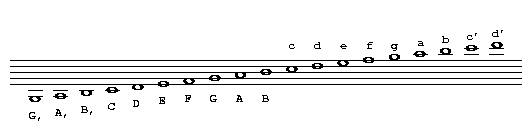
\includegraphics{wiki/_media/abc-standard-pitches.0000.png}}

and by extension other lower and higher notes are available.

Lower octaves are reached by using commas and higher octaves are written
using apostrophes; each extra comma/apostrophe lowers/raises the note by
an octave.

Programs should be able to to parse any combinations of \texttt{,} and
\texttt{\textquotesingle{}} signs appearing after the note. For example
\texttt{C,\textquotesingle{},} (C comma apostrophe comma) has the the
same meaning as \texttt{C,} (C comma) and (uppercase)
\texttt{C\textquotesingle{}} (C apostrophe) should have the same meaning
as (lowercase) \texttt{c}.

Alternatively, it is possible to raise or lower a section of
\protect\hyperlink{music_code_definition}{music code} using the
\texttt{octave} parameter of the \texttt{K:} or \texttt{V:} fields.

\emph{Comment:} The English note names \texttt{C}-\texttt{B}, which are
used in the abc system, correspond to the note names
\texttt{do}-\texttt{si}, which are used in many other languages:
\texttt{do}=\texttt{C}, \texttt{re}=\texttt{D}, \texttt{mi}=\texttt{E},
\texttt{fa}=\texttt{F}, \texttt{sol}=\texttt{G}, \texttt{la}=\texttt{A},
\texttt{si}=\texttt{B}.

\hypertarget{accidentals}{\subsubsection{4.2
Accidentals}\label{accidentals}}

The symbols \texttt{\^{}}, \texttt{=} and \texttt{\_} are used (before a
note) to notate respectively a sharp, natural or flat. Double sharps and
flats are available with \texttt{\^{}\^{}} and \texttt{\_\_}
respectively.

\hypertarget{note_lengths}{\subsubsection{4.3 Note
lengths}\label{note_lengths}}

\emph{Throughout this document note lengths are referred as sixteenth,
eighth, etc. The equivalents common in the U.K. are sixteenth note =
semi-quaver, eighth = quaver, quarter = crotchet and half = minim.}

The \protect\hyperlink{lunit_note_length}{unit note length} for the
transcription is set in the \texttt{L:} field or, if the \texttt{L:}
field does not exist, inferred from the \texttt{M:} field. For example,
\texttt{L:1/8} sets an eighth note as the unit note length.

A single letter in the range \texttt{A-G}, \texttt{a-g} then represents
a note of this length. For example, if the unit note length is an eighth
note, \texttt{DEF} represents 3 eighth notes.

Notes of differing lengths can be obtained by simply putting a
multiplier after the letter. Thus if the unit note length is 1/16,
\texttt{A} or \texttt{A1} is a sixteenth note, \texttt{A2} an eighth
note, \texttt{A3} a dotted eighth note, \texttt{A4} a quarter note,
\texttt{A6} a dotted quarter note, \texttt{A7} a double dotted quarter
note, \texttt{A8} a half note, \texttt{A12} a dotted half note,
\texttt{A14} a double dotted half note, \texttt{A15} a triple dotted
half note and so on. If the unit note length is \texttt{1/8}, \texttt{A}
is an eighth note, \texttt{A2} a quarter note, \texttt{A3} a dotted
quarter note, \texttt{A4} a half note, and so on.

To get shorter notes, either divide them - e.g. if \texttt{A} is an
eighth note, \texttt{A/2} is a sixteenth note, \texttt{A3/2} is a dotted
eighth note, \texttt{A/4} is a thirty-second note - or change the
\protect\hyperlink{lunit_note_length}{unit note length} with the
\texttt{L:} field. Alternatively, if the music has a broken rhythm, e.g.
dotted eighth note/sixteenth note pairs, use
\protect\hyperlink{broken_rhythm}{broken rhythm} markers.

Note that \texttt{A/} is shorthand for \texttt{A/2} and similarly
\texttt{A//} = \texttt{A/4}, etc.

\emph{Comment:} Note lengths that can't be translated to conventional
staff notation are legal, but their representation by abc typesetting
software is undefined and they should be avoided.

\emph{Note for developers:} All compliant software should be able to
handle note lengths down to a 128th note; shorter lengths are optional.

\hypertarget{broken_rhythm}{\subsubsection{4.4 Broken
rhythm}\label{broken_rhythm}}

A common occurrence in traditional music is the use of a dotted or
broken rhythm. For example, hornpipes, strathspeys and certain morris
jigs all have dotted eighth notes followed by sixteenth notes, as well
as vice-versa in the case of strathspeys. To support this, abc notation
uses a \texttt{\textgreater{}} to mean `the previous note is dotted, the
next note halved' and \texttt{\textless{}} to mean `the previous note is
halved, the next dotted'.

\emph{Example:} The following lines all mean the same thing (the third
version is recommended):

\begin{verbatim}
L:1/16
a3b cd3 a2b2c2d2
\end{verbatim}

\begin{verbatim}
L:1/8
a3/2b/2 c/2d3/2 abcd
\end{verbatim}

\begin{verbatim}
L:1/8
a>b c<d abcd
\end{verbatim}

\href{/wiki/_detail/abc:standard:broken-80.png?id=abc\%3Astandard\%3Av2.1}{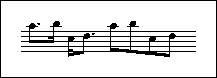
\includegraphics{wiki/_media/abc-standard-broken-80.png}}

As a logical extension, \texttt{\textgreater{}\textgreater{}} means that
the first note is double dotted and the second quartered and
\texttt{\textgreater{}\textgreater{}\textgreater{}} means that the first
note is triple dotted and the length of the second divided by eight.
Similarly for \texttt{\textless{}\textless{}} and
\texttt{\textless{}\textless{}\textless{}}.

Note that the use of broken rhythm markers between notes of unequal
lengths will produce undefined results, and should be avoided.

\hypertarget{rests}{\subsubsection{4.5 Rests}\label{rests}}

Rests can be transcribed with a \texttt{z} or an \texttt{x} and can be
modified in length in exactly the same way as normal notes. \texttt{z}
rests are printed in the resulting sheet music, while \texttt{x} rests
are invisible, that is, not shown in the printed music.

Multi-measure rests are notated using \texttt{Z} (upper case) followed
by the number of measures.

\emph{Example:} The following excerpts, shown with the typeset results,
are musically equivalent (although they are typeset differently).

\begin{verbatim}
Z4|CD EF|GA Bc
\end{verbatim}

\href{/wiki/_detail/abc:standard:rests1-80.png?id=abc\%3Astandard\%3Av2.1}{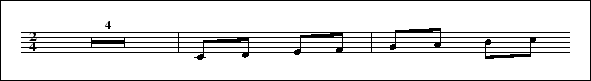
\includegraphics{wiki/_media/abc-standard-rests1-80.png}}

\begin{verbatim}
z4|z4|z4|z4|CD EF|GA Bc
\end{verbatim}

\href{/wiki/_detail/abc:standard:rests2-80.png?id=abc\%3Astandard\%3Av2.1}{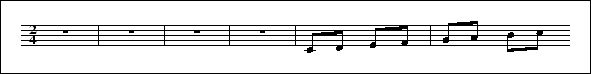
\includegraphics{wiki/_media/abc-standard-rests2-80.png}}

When the number of measures is not given, \texttt{Z} is equivalent to a
pause of one measure.

By extension multi-measure invisible rests are notated using \texttt{X}
(upper case) followed by the number of measures and when the number of
measures is not given, \texttt{X} is equivalent to a pause of one
measure.

\emph{Comment:} Although not particularly valuable, a multi-measure
invisible rest could be useful when a voice is silent for several
measures.

\hypertarget{clefs_and_transposition}{\subsubsection{4.6 Clefs and
transposition}\label{clefs_and_transposition}}

\emph{VOLATILE:} This section is subject to some clarifications with
regard to transposition, rules for the \texttt{middle} parameter and
interactions between different parameters.

Clef and transposition information may be provided in the \texttt{K:}
\protect\hyperlink{kkey}{key} and \texttt{V:}
\protect\hyperlink{multiple_voices}{voice} fields. The general syntax
is:

\begin{verbatim}
[clef=]<clef name>[<line number>][+8 | -8] [middle=<pitch>] [transpose=<semitones>] [octave=<number>] [stafflines=<lines>]
\end{verbatim}

(where \texttt{\textless{}\ldots{}\textgreater{}} denotes a value,
\texttt{{[}\ldots{}{]}} denotes an optional parameter, and
\texttt{\textbar{}} separates alternative values).

\begin{itemize}
\item
  \texttt{\textless{}clef\ name\textgreater{}} - may be \texttt{treble},
  \texttt{alto}, \texttt{tenor}, \texttt{bass}, \texttt{perc} or
  \texttt{none}. \texttt{perc} selects the drum clef. \texttt{clef=} may
  be omitted.
\item
  \texttt{{[}\textless{}line\ number\textgreater{}{]}} - indicates on
  which staff line the base clef is written. Defaults are: treble:
  \texttt{2}; alto: \texttt{3}; tenor: \texttt{4}; bass: \texttt{4}.
\item
  \texttt{{[}+8\ \textbar{}\ -8{]}} - draws `8' above or below the
  staff. The player will transpose the notes one octave higher or lower.
\item
  \texttt{{[}middle=\textless{}pitch\textgreater{}{]}} - is an alternate
  way to define the line number of the clef. The pitch indicates what
  note is displayed on the 3rd line of the staff. Defaults are: treble:
  \texttt{B}; alto: \texttt{C}; tenor: \texttt{A,}; bass: \texttt{D,};
  none: \texttt{B}. This setting does not affect the playback.
\item
  \texttt{{[}transpose=\textless{}semitones\textgreater{}{]}} - for
  playback, transpose the current voice by the indicated amount of
  semitones; positive numbers transpose up, negative down. This setting
  does not affect the printed score. The default is 0.
\item
  \texttt{{[}octave=\textless{}number\textgreater{}{]}} to raise
  (positive number) or lower (negative number) the
  \protect\hyperlink{music_code_definition}{music code} in the current
  voice by one or more octaves. This usage can help to avoid the need to
  write lots of apostrophes or commas to raise or lower notes.
\item
  \texttt{{[}stafflines=\textless{}lines\textgreater{}{]}} - the number
  of lines in the staff. The default is 5.
\end{itemize}

Note that the \texttt{clef}, \texttt{middle}, \texttt{transpose},
\texttt{octave} and \texttt{stafflines} specifiers may be used
independent of each other.

\emph{Examples:}

\begin{verbatim}
K:   clef=alto
K:   perc stafflines=1
K:Am transpose=-2
V:B  middle=d bass
\end{verbatim}

Note that although this standard supports the drum clef, there is
currently no support for special percussion notes.

The middle specifier can be handy when working in the bass clef. Setting
\texttt{K:bass\ middle=d\ transpose=-24} will save you from adding comma
specifiers to the notes (the \texttt{transpose} setting is required to
get the playback sounding at the correct pitch). The specifier may be
abbreviated to \texttt{m=}.

The transpose specifier is useful, for example, for a Bb clarinet, for
which the music is written in the key of C although the instrument plays
it in the key of Bb:

\begin{verbatim}
V:Clarinet
K:C transpose=-2
\end{verbatim}

The transpose specifier may be abbreviated to \texttt{t=}.

To notate the various standard clefs, one can use the following
specifiers:

The seven clefs

\begin{longtable}[]{@{}ll@{}}
\toprule
Name & specifier\tabularnewline
\midrule
\endhead
Treble & \texttt{K:treble}\tabularnewline
Bass & \texttt{K:bass}\tabularnewline
Baritone & \texttt{K:bass3}\tabularnewline
Tenor & \texttt{K:tenor}\tabularnewline
Alto & \texttt{K:alto}\tabularnewline
Mezzosoprano & \texttt{K:alto2}\tabularnewline
Soprano & \texttt{K:alto1}\tabularnewline
\bottomrule
\end{longtable}

More clef names may be allowed in the future, therefore unknown names
should be ignored. If the clef is unknown or not specified, the default
is treble.

Applications may introduce their own clef line specifiers. These
specifiers should start with the name of the application, followed a
colon, followed by the name of the specifier.

\emph{Example:}

\begin{verbatim}
V:p1 perc stafflines=3 m=C  mozart:noteC=snare-drum
\end{verbatim}

\hypertarget{beams}{\subsubsection{4.7 Beams}\label{beams}}

To group notes together under one beam they must be grouped together
without spaces. Thus in 2/4, \texttt{A2BC} will produce an eighth note
followed by two sixteenth notes under one beam whilst \texttt{A2\ B\ C}
will produce the same notes separated. The beam slopes and the choice of
upper or lower stems are typeset automatically.

Notes that cannot be beamed may be placed next to each other. For
example, if \texttt{L:1/8} then \texttt{ABC2DE} is equivalent to
\texttt{AB\ C2\ DE}.

Back quotes \texttt{`} may be used freely between notes to be beamed, to
increase legibility. They are ignored by computer programs. For example,
\texttt{A2``B``C} is equivalent to \texttt{A2BC}.

\hypertarget{repeat_bar_symbols}{\subsubsection{4.8 Repeat/bar
symbols}\label{repeat_bar_symbols}}

Bar line symbols are notated as follows:

\begin{longtable}[]{@{}ll@{}}
\toprule
\textbf{Symbol} & \textbf{Meaning}\tabularnewline
\midrule
\endhead
\texttt{\textbar{}} & bar line\tabularnewline
\texttt{\textbar{}{]}} & thin-thick double bar line\tabularnewline
\texttt{\textbar{}\textbar{}} & thin-thin double bar line\tabularnewline
\texttt{{[}\textbar{}} & thick-thin double bar line\tabularnewline
\texttt{\textbar{}:} & start of repeated section\tabularnewline
\texttt{:\textbar{}} & end of repeated section\tabularnewline
\texttt{::} & start \& end of two repeated sections\tabularnewline
\bottomrule
\end{longtable}

\emph{Recommendation for developers:} If an `end of repeated section' is
found without a previous `start of repeated section', playback programs
should restart the music from the beginning of the tune, or from the
latest double bar line or end of repeated section.

Note that the notation \texttt{::} is short for \texttt{:\textbar{}}
followed by \texttt{\textbar{}:}. The variants \texttt{::},
\texttt{:\textbar{}:} and \texttt{:\textbar{}\textbar{}:} are all
equivalent.

By extension, \texttt{\textbar{}::} and \texttt{::\textbar{}} mean the
start and end of a section that is to be repeated three times, and so
on.

A dotted bar line can be notated by preceding it with a dot, e.g.
\texttt{.\textbar{}} - this may be useful for notating editorial bar
lines in music with very long measures.

An invisible bar line may be notated by putting the bar line in
brackets, e.g. \texttt{{[}\textbar{}{]}} - this may be useful for
notating \protect\hyperlink{voice_overlay}{voice overlay} in meter-free
music.

Abc parsers should be quite liberal in recognizing bar lines. In the
wild, bar lines may have any shape, using a sequence of
\texttt{\textbar{}} (thin bar line), \texttt{{[}} or \texttt{{]}} (thick
bar line), and \texttt{:} (dots), e.g. \texttt{\textbar{}{[}\textbar{}}
or \texttt{{[}\textbar{}:::} .

\hypertarget{first_and_second_repeats}{\subsubsection{4.9 First and
second repeats}\label{first_and_second_repeats}}

First and second repeats can be notated with the symbols \texttt{{[}1}
and \texttt{{[}2}, e.g.

\begin{verbatim}
faf gfe|[1 dfe dBA:|[2 d2e dcB|].
\end{verbatim}

When adjacent to bar lines, these can be shortened to
\texttt{\ \textbar{}1} and \texttt{:\textbar{}2}, but with regard to
spaces

\begin{verbatim}
| [1
\end{verbatim}

is legal, while

\begin{verbatim}
| 1
\end{verbatim}

is not.

Thus, a tune with different ending for the first and second repeats has
the general form:

\begin{verbatim}
|:  <common body of tune>  |1  <first ending>  :|2  <second ending>  |]
\end{verbatim}

Note that in many \protect\hyperlink{abc_file_definition}{abc files} the
\texttt{\textbar{}:} may not be present.

\hypertarget{variant_endings}{\subsubsection{4.10 Variant
endings}\label{variant_endings}}

In combination with \texttt{P:} \protect\hyperlink{pparts}{part
notation}, it is possible to notate more than two variant endings for a
section that is to be repeated a number of times.

For example, if the header of the tune contains \texttt{P:A4.B4} then
parts A and B will each be played 4 times. To play a different ending
each time, you could write in the tune:

\begin{verbatim}
P:A
<notes> | [1  <notes>  :| [2 <notes> :| [3 <notes> :| [4 <notes> |]
\end{verbatim}

The Nth ending starts with \texttt{{[}N} and ends with one of
\texttt{\textbar{}\textbar{}}, \texttt{:\textbar{}}
\texttt{\textbar{}{]}} or \texttt{{[}\textbar{}}. You can also mark a
section as being used for more than one ending e.g.

\begin{verbatim}
[1,3 <notes> :|
\end{verbatim}

plays on the 1st and 3rd endings and

\begin{verbatim}
[1-3 <notes> :|
\end{verbatim}

plays on endings 1, 2 and 3. In general, `{[}' can be followed by any
list of numbers and ranges as long as it contains no spaces e.g.

\begin{verbatim}
[1,3,5-7  <notes>  :| [2,4,8 <notes> :|
\end{verbatim}

\hypertarget{ties_and_slurs}{\subsubsection{4.11 Ties and
slurs}\label{ties_and_slurs}}

You can tie two notes of the same pitch together, within or between
bars, with a \texttt{-} symbol, e.g. \texttt{abc-\textbar{}cba} or
\texttt{c4-c4}. The tie symbol must always be adjacent to the first note
of the pair, but does not need to be adjacent to the second, e.g.
\texttt{c4\ -c4} and \texttt{abc\textbar{}-cba} are not legal - see
\protect\hyperlink{order_of_abc_constructs}{order of abc constructs}.

More general slurs can be put in with \texttt{()} symbols. Thus
\texttt{(DEFG)} puts a slur over the four notes. Spaces within a slur
are OK, e.g. \texttt{\ (\ D\ E\ F\ G\ )\ }.

Slurs may be nested:

\begin{verbatim}
(c (d e f) g a)
\end{verbatim}

\href{/wiki/_detail/abc:standard:slur1-80.png?id=abc\%3Astandard\%3Av2.1}{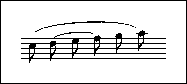
\includegraphics{wiki/_media/abc-standard-slur1-80.png}}

and they may also start and end on the same note:

\begin{verbatim}
(c d (e) f g a)
\end{verbatim}

\href{/wiki/_detail/abc:standard:slur2-80.png?id=abc\%3Astandard\%3Av2.1}{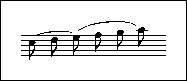
\includegraphics{wiki/_media/abc-standard-slur2-80.png}}

A dotted slur may be notated by preceding the opening brace with a dot,
e.g. \texttt{.(cde)}; it is optional to place a dot immediately before
the closing brace. Likewise, a dotted tie can be transcribed by
preceding it with a dot, e.g. \texttt{C.-C}. This is especially useful
in parts with multiple verses: some verses may require a slur, some may
not.

It should be noted that although the tie \texttt{-} and slur \texttt{()}
produce similar symbols in staff notation they have completely different
meanings to player programs and should not be interchanged. Ties connect
two successive notes \emph{of the same pitch}, causing them to be played
as a single note, while slurs connect the first and last note of any
series of notes, and may be used to indicate phrasing, or that the group
should be played legato. Both ties and slurs may be used into, out of
and between chords, and in this case the distinction between them is
particularly important.

\hypertarget{grace_notes}{\subsubsection{4.12 Grace
notes}\label{grace_notes}}

Grace notes can be written by enclosing them in curly braces,
\texttt{\{\}}. For example, a taorluath on the Highland pipes would be
written \texttt{\{GdGe\}}. The tune `Athol Brose' (in the file
\protect\hyperlink{strspysabc}{Strspys.abc}) has an example of complex
Highland pipe gracing in all its glory. Although nominally grace notes
have no melodic time value, expressions such as \texttt{\{a3/2b/\}} or
\texttt{\{a\textgreater{}b\}} can be useful and are legal although some
software may ignore them. The unit duration to use for gracenotes is not
specified by the \protect\hyperlink{abc_file_definition}{abc file}, but
by the software, and might be a specific amount of time (for playback
purposes) or a note length (e.g. 1/32 for Highland pipe music, which
would allow \texttt{\{ge4d\}} to code a piobaireachd `cadence').

To distinguish between appoggiaturas and acciaccaturas, the latter are
notated with a forward slash immediately following the open brace, e.g.
\texttt{\{/g\}C} or \texttt{\{/gagab\}C}:

\href{/wiki/_detail/abc:standard:graces-80.png?id=abc\%3Astandard\%3Av2.1}{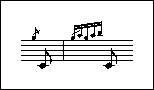
\includegraphics{wiki/_media/abc-standard-graces-80.png}}

The presence of gracenotes is transparent to the broken rhythm
construct. Thus the forms \texttt{A\textless{}\{g\}A} and
\texttt{A\{g\}\textless{}A} are legal and equivalent to
\texttt{A/2\{g\}A3/2}.

\hypertarget{duplets_triplets_quadruplets_etc}{\subsubsection{4.13
Duplets, triplets, quadruplets,
etc.}\label{duplets_triplets_quadruplets_etc}}

These can be simply coded with the notation \texttt{(2ab} for a duplet,
\texttt{(3abc} for a triplet or \texttt{(4abcd} for a quadruplet, etc,
up to \texttt{(9}. The musical meanings are:

\begin{longtable}[]{@{}ll@{}}
\toprule
\textbf{Symbol} & \textbf{Meaning}\tabularnewline
\midrule
\endhead
\texttt{(2} & 2 notes in the time of 3\tabularnewline
\texttt{(3} & 3 notes in the time of 2\tabularnewline
\texttt{(4} & 4 notes in the time of 3\tabularnewline
\texttt{(5} & 5 notes in the time of \emph{n}\tabularnewline
\texttt{(6} & 6 notes in the time of 2\tabularnewline
\texttt{(7} & 7 notes in the time of \emph{n}\tabularnewline
\texttt{(8} & 8 notes in the time of 3\tabularnewline
\texttt{(9} & 9 notes in the time of \emph{n}\tabularnewline
\bottomrule
\end{longtable}

If the time signature is compound (6/8, 9/8, 12/8) then \emph{n} is
three, otherwise \emph{n} is two.

More general tuplets can be specified using the syntax \texttt{(p:q:r}
which means 'put \emph{p} notes into the time of \emph{q} for the next
\emph{r} notes'. If \emph{q} is not given, it defaults as above. If
\emph{r} is not given, it defaults to \emph{p}.

For example, \texttt{(3} is equivalent to \texttt{(3::} or \texttt{(3:2}
, which in turn are equivalent to \texttt{(3:2:3}, whereas
\texttt{(3::2} is equivalent to \texttt{(3:2:2}.

This can be useful to include notes of different lengths within a
tuplet, for example \texttt{(3:2:2\ G4c2} or \texttt{(3:2:4\ G2A2Bc}. It
also describes more precisely how the simple syntax works in cases like
\texttt{(3\ D2E2F2} or even \texttt{(3\ D3EF2}. The number written over
the tuplet is \emph{p}.

Spaces that appear between the tuplet specifier and the following notes
are to be ignored.

\hypertarget{decorations}{\subsubsection{4.14
Decorations}\label{decorations}}

A number of shorthand decoration symbols are available:

\begin{verbatim}
.       staccato mark
~       Irish roll
H       fermata
L       accent or emphasis
M       lowermordent
O       coda
P       uppermordent
S       segno
T       trill
u       up-bow
v       down-bow
\end{verbatim}

Decorations should be placed before the note which they decorate - see
\protect\hyperlink{order_of_abc_constructs}{order of abc constructs}

\emph{Examples:}

\begin{verbatim}
(3.a.b.c    % staccato triplet
vAuBvA      % bowing marks (for fiddlers)
\end{verbatim}

Most of the characters above (\texttt{\textasciitilde{}HLMOPSTuv}) are
just short-cuts for commonly used decorations and can even be redefined
(see \protect\hyperlink{redefinable_symbols}{redefinable symbols}).

More generally, symbols can be entered using the syntax
\texttt{!symbol!}, e.g. \texttt{!trill!A4} for a trill symbol. (Note
that the abc standard version 2.0 used instead the syntax
\texttt{+symbol+} - this dialect of abc is still available, but is now
\protect\hyperlink{outdated_syntax}{deprecated} - see
\protect\hyperlink{decoration_dialects}{decoration dialects}.)

The currently defined symbols are:

\begin{verbatim}
!trill!                "tr" (trill mark)
!trill(!               start of an extended trill
!trill)!               end of an extended trill
!lowermordent!         short /|/|/ squiggle with a vertical line through it
!uppermordent!         short /|/|/ squiggle
!mordent!              same as !lowermordent!
!pralltriller!         same as !uppermordent!
!roll!                 a roll mark (arc) as used in Irish music
!turn!                 a turn mark (also known as gruppetto)
!turnx!                a turn mark with a line through it
!invertedturn!         an inverted turn mark
!invertedturnx!        an inverted turn mark with a line through it
!arpeggio!             vertical squiggle
!>!                    > mark
!accent!               same as !>!
!emphasis!             same as !>!
!fermata!              fermata or hold (arc above dot)
!invertedfermata!      upside down fermata
!tenuto!               horizontal line to indicate holding note for full duration
!0! - !5!              fingerings
!+!                    left-hand pizzicato, or rasp for French horns
!plus!                 same as !+!
!snap!                 snap-pizzicato mark, visually similar to !thumb!
!slide!                slide up to a note, visually similar to a half slur
!wedge!                small filled-in wedge mark
!upbow!                V mark
!downbow!              squared n mark
!open!                 small circle above note indicating open string or harmonic
!thumb!                cello thumb symbol
!breath!               a breath mark (apostrophe-like) after note
!pppp! !ppp! !pp! !p!  dynamics marks
!mp! !mf! !f! !ff!     more dynamics marks
!fff! !ffff! !sfz!     more dynamics marks
!crescendo(!           start of a < crescendo mark
!<(!                   same as !crescendo(!
!crescendo)!           end of a < crescendo mark, placed after the last note
!<)!                   same as !crescendo)!
!diminuendo(!          start of a > diminuendo mark
!>(!                   same as !diminuendo(!
!diminuendo)!          end of a > diminuendo mark, placed after the last note
!>)!                   same as !diminuendo)!
!segno!                2 ornate s-like symbols separated by a diagonal line
!coda!                 a ring with a cross in it
!D.S.!                 the letters D.S. (=Da Segno)
!D.C.!                 the letters D.C. (=either Da Coda or Da Capo)
!dacoda!               the word "Da" followed by a Coda sign
!dacapo!               the words "Da Capo"
!fine!                 the word "fine"
!shortphrase!          vertical line on the upper part of the staff
!mediumphrase!         same, but extending down to the centre line
!longphrase!           same, but extending 3/4 of the way down
\end{verbatim}

Here is a picture of most decorations:

\href{/wiki/_detail/abc:standard:decorations.0000.png?id=abc\%3Astandard\%3Av2.1}{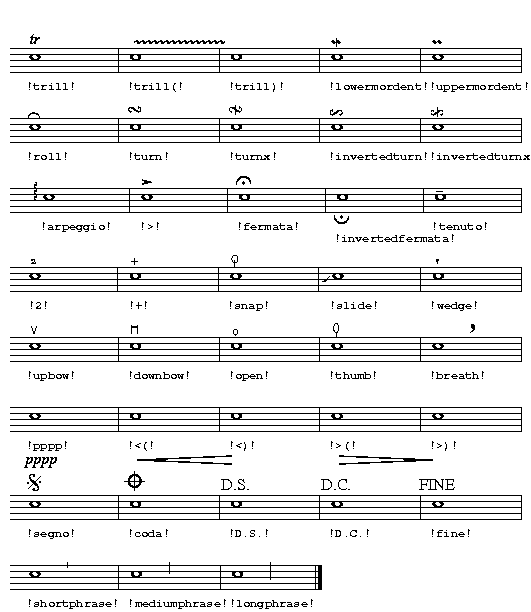
\includegraphics{wiki/_media/abc-standard-decorations.0000.png}}

Note that the decorations may be applied to notes, rests, note groups,
and bar lines. If a decoration is to be typeset between notes, it may be
attached to the \texttt{y} spacer - see
\protect\hyperlink{typesetting_extra_space}{typesetting extra space}.

Spaces may be used freely between each of the symbols and the object to
which it should be attached. Also an object may be preceded by multiple
symbols, which should be printed one over another, each on a different
line.

\emph{Example:}

\begin{verbatim}
[!1!C!3!E!5!G]  !coda! y  !p! !trill! C   !fermata!|
\end{verbatim}

\href{/wiki/_detail/abc:standard:decorations2-80.png?id=abc\%3Astandard\%3Av2.1}{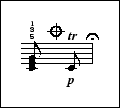
\includegraphics{wiki/_media/abc-standard-decorations2-80.png}}

Player programs may choose to ignore most of the symbols mentioned
above, though they may be expected to implement the dynamics marks, the
accent mark and the staccato dot. Default volume is equivalent to !mf!.
On a scale from 0-127, the relative volumes can be roughly defined as:
\texttt{!pppp!} = \texttt{!ppp!} = 30, \texttt{!pp!} = 45, \texttt{!p!}
= 60, \texttt{!mp!} = 75, \texttt{!mf!} = 90, \texttt{!f!} = 105,
\texttt{!ff!} = 120, \texttt{!fff!} = \texttt{!ffff!} = 127.

Abc software may also allow users to define new symbols in a package
dependent way.

Note that symbol names may not contain any spaces, \texttt{{[}},
\texttt{{]}}, \texttt{\textbar{}} or \texttt{:} signs, e.g. while
!dacapo! is legal, !da capo! is not.

If an unimplemented or unknown symbol is found, it should be ignored.

\emph{Recommendation:} A good source of general information about
decorations can be found at
\url{http://www.dolmetsch.com/musicalsymbols.htm}.

\hypertarget{symbol_lines}{\subsubsection{4.15 Symbol
lines}\label{symbol_lines}}

Adding many symbols to a line of music can make a tune difficult to
read. In such cases, a symbol line (a line that contains only
\texttt{!\ldots{}!} \protect\hyperlink{decorations}{decorations},
\texttt{"\ldots{}"} \protect\hyperlink{chord_symbols}{chord symbols} or
\protect\hyperlink{annotations}{annotations}) can be used, analogous to
a line of \protect\hyperlink{lyrics}{lyrics}.

A symbol line starts with \texttt{s:}, followed by a line of symbols.
Matching of notes and symbols follow the
\protect\hyperlink{alignment}{alignment rules} defined for lyrics
(meaning that symbols in an \texttt{s:} line cannot be aligned on
\protect\hyperlink{grace_notes}{grace notes},
\protect\hyperlink{rests}{rests} or
\protect\hyperlink{typesetting_extra_space}{spacers}).

\emph{Example:}

\begin{verbatim}
   CDEF    | G```AB`c
s: "^slow" | !f! ** !fff!
\end{verbatim}

It is also possible to stack \texttt{s:} lines to produced multiple
symbols on a note.

\emph{Example:} The following two excerpts are equivalent and would
place a decorations plus a chord on the \texttt{E}.

\begin{verbatim}
   C2  C2 Ez   A2|
s: "C" *  "Am" * |
s: *   *  !>!  * |
\end{verbatim}

\begin{verbatim}
"C" C2 C2 "Am" !>! Ez A2|
\end{verbatim}

\hypertarget{redefinable_symbols}{\subsubsection{4.16 Redefinable
symbols}\label{redefinable_symbols}}

As a short cut to writing symbols which avoids the \texttt{!symbol!}
syntax (see \protect\hyperlink{decorations}{decorations}), the letters
\texttt{H-W} and \texttt{h-w} and the symbol \texttt{\textasciitilde{}}
can be assigned with the \texttt{U:} field. For example, to assign the
letter \texttt{T} to represent the trill, you can write:

\begin{verbatim}
U: T = !trill!
\end{verbatim}

You can also use \texttt{"\^{}text"}, etc (see
\protect\hyperlink{annotations}{annotations} below) in definitions

\emph{Example:} To print a plus sign over notes, define \texttt{p} as
follows and use it before the required notes:

\begin{verbatim}
U: p = "^+"
\end{verbatim}

Symbol definitions can be written in the
\protect\hyperlink{file_header_definition}{file header}, in which case
they apply to all the tunes in that file, or in a
\protect\hyperlink{tune_header_definition}{tune header}, when they apply
only to that tune, and override any previous definitions. Programs may
also make use of a set of global default definitions, which apply
everywhere unless overridden by local definitions. You can assign the
same symbol to two or more letters e.g.

\begin{verbatim}
U: T = !trill!
U: U = !trill!
\end{verbatim}

in which case the same visible symbol will be produced by both letters
(but they may be played differently), and you can de-assign a symbol by
writing:

\begin{verbatim}
U: T = !nil!
\end{verbatim}

or

\begin{verbatim}
U: T = !none!
\end{verbatim}

The standard set of definitions (if you do not redefine them) is:

\begin{verbatim}
U: ~ = !roll!
U: H = !fermata!
U: L = !accent!
U: M = !lowermordent!
U: O = !coda!
U: P = !uppermordent!
U: S = !segno!
U: T = !trill!
U: u = !upbow!
U: v = !downbow!
\end{verbatim}

Please see \protect\hyperlink{macros}{macros} for an advanced macro
mechanism.

\hypertarget{chords_and_unisons}{\subsubsection{4.17 Chords and
unisons}\label{chords_and_unisons}}

Chords (i.e. more than one note head on a single stem) can be coded with
\texttt{{[}{]}} symbols around the notes, e.g.

\begin{verbatim}
[CEGc]
\end{verbatim}

indicates the chord of C major. They can be grouped in beams, e.g.

\begin{verbatim}
[d2f2][ce][df]
\end{verbatim}

but there should be no spaces within the notation for a chord. See the
tune `Kitchen Girl' in the sample file
\protect\hyperlink{reelsabc}{Reels.abc} for a simple example.

All the notes within a chord should normally have the same length, but
if not, the chord duration is that of the first note.

\emph{Recommendation:} Although playback programs should not have any
difficulty with notes of different lengths, typesetting programs may not
always be able to render the resulting chord to staff notation (for
example, an eighth and a quarter note cannot be represented on the same
stem) and the result is undefined. Consequently, this is not
recommended.

More complicated chords can be transcribed with the \texttt{\&} operator
(see \protect\hyperlink{voice_overlay}{voice overlay}).

The chord forms a syntactic grouping, to which the same prefixes and
postfixes can be attached as to an ordinary note (except for accidentals
which should be attached to individual notes within the chord and
decorations which may be attached to individual notes within the chord
or may be attached to the chord as a whole).

\emph{Example:}

\begin{verbatim}
( "^I" !f! [CEG]- > [CEG] "^IV" [F=AC]3/2"^V"[GBD]/  H[CEG]2 )
\end{verbatim}

\href{/wiki/_detail/abc:standard:chords-80.png?id=abc\%3Astandard\%3Av2.1}{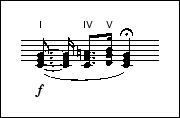
\includegraphics{wiki/_media/abc-standard-chords-80.png}}

When both inside and outside the chord length modifiers are used, they
should be multiplied. \emph{Example:} \texttt{{[}C2E2G2{]}3} has the
same meaning as \texttt{{[}CEG{]}6}.

If the chord contains two notes of the same pitch, then it is a unison
(e.g. a note played on two strings of a violin simultaneously) and is
shown with one stem and two note-heads.

\emph{Example:}

\begin{verbatim}
[DD]
\end{verbatim}

\href{/wiki/_detail/abc:standard:unison-80.png?id=abc\%3Astandard\%3Av2.1}{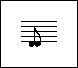
\includegraphics{wiki/_media/abc-standard-unison-80.png}}

\hypertarget{chord_symbols}{\subsubsection{4.18 Chord
symbols}\label{chord_symbols}}

\emph{VOLATILE:} The list of chords and how they are handled will be
extended at some point. Until then programs should treat chord symbols
quite liberally.

Chord symbols (e.g. chords/bass notes) can be put in under the melody
line (or above, depending on the package) using double-quotation marks
placed to the left of the note it is sounded with, e.g.
\texttt{"Am7"A2D2}.

The chord has the format
\emph{\textless{}note\textgreater{}\textless{}accidental\textgreater{}\textless{}type\textgreater{}\textless{}/bass\textgreater{}},
where \emph{\textless{}note\textgreater{}} can be \texttt{A-G}, the
optional \emph{\textless{}accidental\textgreater{}} can be \texttt{b},
\texttt{\#}, the optional \emph{\textless{}type\textgreater{}} is one or
more of

\begin{verbatim}
m or min        minor
maj             major
dim             diminished
aug or +        augmented
sus             suspended
7, 9 ...        7th, 9th, etc.
\end{verbatim}

and \emph{\textless{}/bass\textgreater{}} is an optional bass note.

A slash after the chord type is used only if the optional bass note is
also used, e.g., \texttt{"C/E"}. If the bass note is a regular part of
the chord, it indicates the inversion, i.e., which note of the chord is
lowest in pitch. If the bass note is not a regular part of the chord, it
indicates an additional note that should be sounded with the chord,
below it in pitch. The bass note can be any letter (\texttt{A-G} or
\texttt{a-g}), with or without a trailing accidental sign (\texttt{b} or
\texttt{\#}). The case of the letter used for the bass note does not
affect the pitch.

Alternate chords can be indicated for printing purposes (but not for
playback) by enclosing them in parentheses inside the double-quotation
marks after the regular chord, e.g., \texttt{"G(Em)"}.

\emph{Note to developers:} Software should also be able to recognise and
handle appropriately the unicode versions of flat, natural and sharp
symbols (♭, ♮, ♯) - see \protect\hyperlink{special_symbols}{special
symbols}.

\hypertarget{annotations}{\subsubsection{4.19
Annotations}\label{annotations}}

General text annotations can be added above, below or on the staff in a
similar way to chord symbols. In this case, the string within double
quotes is preceded by one of five symbols \texttt{\^{}}, \texttt{\_},
\texttt{\textless{}}, \texttt{\textgreater{}} or \texttt{@} which
controls where the annotation is to be placed; above, below, to the left
or right respectively of the following note, rest or bar line. Using the
\texttt{@} symbol leaves the exact placing of the string to the
discretion of the interpreting program. These placement specifiers
distinguish annotations from chord symbols, and should prevent programs
from attempting to play or transpose them. All text that follows the
placement specifier is treated as a
\protect\hyperlink{text_string_definition}{text string}.

Where two or more annotations with the same placement specifier are
placed consecutively, e.g. for fingerings, the notation program should
draw them on separate lines, with the first listed at the top.

\emph{Example:} The following annotations place the note between
parentheses.

\begin{verbatim}
"<(" ">)" C
\end{verbatim}

\hypertarget{order_of_abc_constructs}{\subsubsection{4.20 Order of abc
constructs}\label{order_of_abc_constructs}}

The order of abc constructs for a note is: \emph{\textless{}grace
notes\textgreater{}}, \emph{\textless{}chord symbols\textgreater{}},
\emph{\textless{}annotations\textgreater{}/\textless{}decorations\textgreater{}}
(e.g. Irish roll, staccato marker or up/downbow),
\emph{\textless{}accidentals\textgreater{}},
\emph{\textless{}note\textgreater{}},
\emph{\textless{}octave\textgreater{}}, \emph{\textless{}note
length\textgreater{}}, i.e.
\texttt{\textasciitilde{}\^{}c\textquotesingle{}3} or even
\texttt{"Gm7"v.=G,2}.

Each \protect\hyperlink{ties_and_slurs}{tie symbol}, \texttt{-}, should
come immediately after a note group but may be followed by a space, i.e.
\texttt{=G,2-\ }. Open and close chord delimiters, \texttt{{[}} and
\texttt{{]}}, should enclose entire note sequences (except for chord
symbols), e.g.

\begin{verbatim}
"C"[CEGc]|
|"Gm7"[.=G,^c']
\end{verbatim}

and open and close slur symbols, \texttt{()}, should do likewise, i.e.

\begin{verbatim}
"Gm7"(v.=G,2~^c'2)
\end{verbatim}

\begin{center}\rule{0.5\linewidth}{\linethickness}\end{center}

\hypertarget{lyrics}{\subsection{5. Lyrics}\label{lyrics}}

The \texttt{W:}
\protect\hyperlink{information_field_definition}{information field}
(uppercase W) can be used for lyrics to be printed separately below the
tune.

The \texttt{w:}
\protect\hyperlink{information_field_definition}{information field}
(lowercase w) in the \protect\hyperlink{tune_body_definition}{tune
body}, supplies lyrics to be aligned syllable by syllable with previous
notes of the current voice.

\hypertarget{alignment}{\subsubsection{5.1 Alignment}\label{alignment}}

When adjacent, \texttt{w:} fields indicate different verses
(\protect\hyperlink{verses}{see below}), but for non-adjacent
\texttt{w:} fields, the alignment of the lyrics:

\begin{itemize}
\item
  starts at the first note of the voice if there is no previous
  \texttt{w:} field; or
\item
  starts at the first note after the notes aligned to the previous
  \texttt{w:} field; and
\item
  associates syllables to notes up to the end of the \texttt{w:} line.
\end{itemize}

\emph{Example:} The following two examples are equivalent.

\begin{verbatim}
C D E F|
w: doh re mi fa
G A B c|
w: sol la ti doh
\end{verbatim}

\begin{verbatim}
C D E F|
G A B c|
w: doh re mi fa sol la ti doh
\end{verbatim}

\emph{Comment:} The second example, made possible by an extension
(introduced in abc 2.1) of the alignment rules, means that lyrics no
longer have to follow immediately after the line of notes to which they
are attached. Indeed, the placement of the lyrics can be postponed to
the end of the \protect\hyperlink{tune_body_definition}{tune body}.
However, the extension of the alignment rules is not fully backwards
compatible with abc 2.0 - see
\protect\hyperlink{outdated_lyrics_alignment}{outdated lyrics alignment}
for an explanation.

If there are fewer syllables than available notes, the remaining notes
have no lyric (blank syllables); thus the appearance of a \texttt{w:}
field associates all the notes that have appeared previously with a
syllable (either real or blank).

\emph{Example:} In the following example the empty \texttt{w:} field
means that the 4 \texttt{G} notes have no lyric associated with them.

\begin{verbatim}
C D E F|
w: doh re mi fa
G G G G|
w:
F E F C|
w: fa mi re doh
\end{verbatim}

If there are more syllables than available notes, any excess syllables
will be ignored.

\emph{Recommendation for developers:} If a \texttt{w:} line does not
contain the correct number of syllables for the corresponding notes, the
program should warn the user. However, having insufficient syllables is
legitimate usage (as above) and so the program may allow these warnings
to be switched off.

Note that syllables are not aligned on
\protect\hyperlink{grace_notes}{grace notes},
\protect\hyperlink{rests}{rests} or
\protect\hyperlink{typesetting_extra_space}{spacers} and that tied,
slurred or beamed notes are treated as separate notes in this context.

The lyrics lines are treated as
\protect\hyperlink{text_string_definition}{text strings}. Within the
lyrics, the words should be separated by one or more spaces and to
correctly align them the following symbols may be used:

\begin{longtable}[]{@{}ll@{}}
\toprule
\textbf{Symbol} & \textbf{Meaning}\tabularnewline
\midrule
\endhead
\texttt{-} & (hyphen) break between syllables within a
word\tabularnewline
\texttt{\_} & (underscore) previous syllable is to be held for an extra
note\tabularnewline
\texttt{*} & one note is skipped (i.e. * is equivalent to a blank
syllable)\tabularnewline
\texttt{\textasciitilde{}} & appears as a space; aligns multiple words
under one note\tabularnewline
\texttt{\textbackslash{}-} & appears as hyphen; aligns multiple
syllables under one note\tabularnewline
\texttt{\textbar{}} & advances to the next bar\tabularnewline
\bottomrule
\end{longtable}

Note that if \texttt{-} is preceded by a space or another hyphen, the
\texttt{-} is regarded as a separate syllable.

When an underscore is used next to a hyphen, the hyphen must always come
first.

If there are not as many syllables as notes in a measure, typing a
\texttt{\textbar{}} automatically advances to the next bar; if there are
enough syllables the \texttt{\textbar{}} is just ignored.

\emph{Examples:}

\begin{verbatim}
w: syll-a-ble    is aligned with three notes
w: syll-a--ble   is aligned with four notes
w: syll-a -ble   (equivalent to the previous line)
w: time__        is aligned with three notes
w: of~the~day    is treated as one syllable (i.e. aligned with one note)
                 but appears as three separate words
\end{verbatim}

\begin{verbatim}
 gf|e2dc B2A2|B2G2 E2D2|.G2.G2 GABc|d4 B2
w: Sa-ys my au-l' wan to your aul' wan,
+: Will~ye come to the Wa-x-ies dar-gle?
\end{verbatim}

See \protect\hyperlink{field_continuation}{field continuation} for the
meaning of the \texttt{+:} field continuation.

\hypertarget{verses}{\subsubsection{5.2 Verses}\label{verses}}

It is possible for a music line to be followed by several adjacent
\texttt{w:} fields, i.e. immediately after each other. This can be used,
together with part notation, to represent different verses. The first
\texttt{w:} field is used the first time that part is played, then the
second and so on.

\emph{Examples:} The following two examples are equivalent and contain
two verses:

\begin{verbatim}
CDEF FEDC|
w: these are the lyr-ics for verse one
w: these are the lyr-ics for verse two
\end{verbatim}

\begin{verbatim}
CDEF FEDC|
w: these are the lyr-ics
+:  for verse one
w: these are the lyr-ics
+:  for verse two  
\end{verbatim}

\hypertarget{numbering}{\subsubsection{5.3 Numbering}\label{numbering}}

\emph{VOLATILE:} The following syntax may be extended to include
non-numeric ``numbering''.

If the first word of a \texttt{w:} line starts with a digit, this is
interpreted as numbering of a stanza. Typesetting programs should align
the corresponding note with the first letter that occurs. This can be
used in conjunction with the \texttt{\textasciitilde{}} symbol mentioned
in the table above to create a space between the digit and the first
letter.

\emph{Example:} In the following, the \texttt{1.\textasciitilde{}Three}
is treated as a single word with a space created by the
\texttt{\textasciitilde{}}, but the fact that the \texttt{w:} line
starts with a number means that the first note of the corresponding
music line is aligned to \texttt{Three}.

\begin{verbatim}
   w: 1.~Three blind mice
\end{verbatim}

\begin{center}\rule{0.5\linewidth}{\linethickness}\end{center}

\hypertarget{typesetting_and_playback}{\subsection{6. Typesetting and
playback}\label{typesetting_and_playback}}

\hypertarget{typesetting}{\subsubsection{6.1
Typesetting}\label{typesetting}}

\hypertarget{typesetting_line-breaks}{\paragraph{6.1.1 Typesetting
line-breaks}\label{typesetting_line-breaks}}

\emph{Terminology:} \textbf{Line-breaks} in a document (also known in
computing as new lines, line-feeds, carriage-returns, end-of-lines,
etc.) determine how the document is set out on the page. Throughout this
section, and elsewhere in the standard, a distinction should be noted
between

\begin{itemize}
\item
  \href{}{}a \textbf{code line-break}, meaning a line-break in the abc
  \protect\hyperlink{tune_body_definition}{tune body}, and, in
  particular, at the end of a line of
  \protect\hyperlink{music_code_definition}{music code};
\item
  \href{}{}a \textbf{score line-break}, meaning a line-break in the
  printed score.
\end{itemize}

The fundamental mechanism for typesetting
\protect\hyperlink{score_line-break_definition}{score line-breaks} is by
using \protect\hyperlink{code_line-break_definition}{code line-breaks} -
one line of \protect\hyperlink{music_code_definition}{music code} in the
\protect\hyperlink{tune_body_definition}{tune body} normally corresponds
to one line of printed music.

Of course the printed representation of a line of
\protect\hyperlink{music_code_definition}{music code} may be too long
for the staff, so if necessary, typesetting programs should introduce
additional \protect\hyperlink{score_line-break_definition}{score
line-breaks}. As a consequence, if you would prefer
\protect\hyperlink{score_line-break_definition}{score line-breaks} to be
handled completely automatically (as is common in non-abc scoring
software), then just type the
\protect\hyperlink{tune_body_definition}{tune body} on a single line of
\protect\hyperlink{music_code_definition}{music code}.

Even though most abc GUI software should wrap over-long lines, typing
the \protect\hyperlink{tune_body_definition}{tune body} on a single line
may not always be convenient, particularly for users who wish to include
\protect\hyperlink{code_line-break_definition}{code line-breaks} to aid
readability or if the abc code is to be emailed (see
\protect\hyperlink{continuation_of_input_lines}{continuation of input
lines}).

Furthermore, in the past some typesetting programs used \texttt{!}
characters in the abc code to force
\protect\hyperlink{score_line-break_definition}{score line-breaks}.

As a result, abc 2.1 introduces a new line-breaking instruction.

\subparagraph{I:linebreak}\label{ilinebreak}

To allow for all line-breaking preferences, the \texttt{I:linebreak}
instruction may be used, together with four possible values, to control
\protect\hyperlink{score_line-break_definition}{score line-breaking}.

\begin{itemize}
\item
  "\texttt{I:linebreak\ \$}" indicates that the \texttt{\$} symbol is
  used in the \protect\hyperlink{tune_body_definition}{tune body} to
  typeset a \protect\hyperlink{score_line-break_definition}{score
  line-break}. Any \protect\hyperlink{code_line-break_definition}{code
  line-breaks} are ignored for typesetting purposes.
\end{itemize}

\emph{Example:} The following abc code should be typeset on two lines.

\begin{verbatim}
I:linebreak $
K:G
|:abc def|$fed cba:|
\end{verbatim}

\begin{itemize}
\item
  "\texttt{I:linebreak\ !}" indicates that the \texttt{!} symbol is used
  to typeset a \protect\hyperlink{score_line-break_definition}{score
  line-break}. Any \protect\hyperlink{code_line-break_definition}{code
  line-breaks} are ignored for typesetting purposes.
\end{itemize}

\emph{Comment:} The "\texttt{I:linebreak\ !}" instruction works in the
same way as \texttt{I:linebreak\ \$} and is primarily provided for
backwards compatibility - see
\protect\hyperlink{line-breaking_dialects}{line-breaking dialects}, so
that "\texttt{I:linebreak\ \$}" is the preferred usage.
"\texttt{I:linebreak\ !}" also automatically invokes the
"\texttt{I:decoration\ +}" instruction - see
\protect\hyperlink{decoration_dialects}{decoration dialects}. Finally,
"\texttt{I:linebreak\ !}" is equivalent to the
\protect\hyperlink{outdated_syntax}{deprecated} directive
\texttt{\%\%continueall\ true} - see
\protect\hyperlink{outdated_directives}{outdated directives}.

\begin{itemize}
\item
  "\texttt{I:linebreak\ \textless{}EOL\textgreater{}}" indicates that
  the End Of Line character (CR, LF or CRLF) is used to typeset a
  \protect\hyperlink{score_line-break_definition}{score line-break}. In
  other words, \protect\hyperlink{code_line-break_definition}{code
  line-breaks} are used for typesetting
  \protect\hyperlink{score_line-break_definition}{score line-breaks}.
\end{itemize}

\begin{itemize}
\item
  "\texttt{I:linebreak\ \textless{}none\textgreater{}}" indicates that
  all line-breaking is to be carried out automatically and any
  \protect\hyperlink{code_line-break_definition}{code line-breaks} are
  ignored for typesetting purposes.
\end{itemize}

The values \texttt{\textless{}EOL\textgreater{}}, \texttt{\$} and
\texttt{!} may also be combined so that more that one symbol can
indicate a \protect\hyperlink{score_line-break_definition}{score
line-break}.

The default line-break setting is:

\begin{verbatim}
I:linebreak <EOL> $
\end{verbatim}

meaning that both \protect\hyperlink{code_line-break_definition}{code
line-breaks}, and \texttt{\$} symbols, generate a
\protect\hyperlink{score_line-break_definition}{score line-break}.

\emph{Comment:} Although "\texttt{I:linebreak\ \$\ !}" is legal it is
not recommended as it uses two different symbols to mean the same thing.

An \texttt{I:linebreak} instruction can be used either in the
\protect\hyperlink{file_header_definition}{file header} (in which case
it is applied to every \protect\hyperlink{abc_tune_definition}{tune} in
the \protect\hyperlink{abc_file_definition}{abc file}), or in a
\protect\hyperlink{tune_header_definition}{tune header} (in which case
it is applied to that tune only and overrides a line-breaking
instruction in the \protect\hyperlink{file_header_definition}{file
header}). Similarly, if two \texttt{I:linebreak} instructions appear in
a \protect\hyperlink{file_header_definition}{file header} or a
\protect\hyperlink{tune_header_definition}{tune header}, the second
cancels the first.

\emph{Comment:} It can be sometimes be useful to include two
instructions together - for example,
"\texttt{I:linebreak\ \textless{}EOL\textgreater{}\ \$}" and
"\texttt{I:linebreak\ \textless{}none\textgreater{}}" can be used to
toggle between default and automatic line-breaking simply by swapping
the position of the two lines.

\texttt{I:linebreak} instructions are not allowed in the
\protect\hyperlink{tune_body_definition}{tune body} (principally because
it conflicts with the human readability of the
\protect\hyperlink{music_code_definition}{music code}).

\subparagraph{Suppressing score
line-breaks}\label{suppressing_score_line-breaks}

When the \texttt{\textless{}EOL\textgreater{}} character is being used
in the \protect\hyperlink{tune_body_definition}{tune body} to indicate
\protect\hyperlink{score_line-break_definition}{score line-breaks}, it
sometimes useful to be able to tell typesetting software to ignore a
particular \protect\hyperlink{code_line-break_definition}{code
line-breaks}. This is achieved using a backslash
(\texttt{\textbackslash{}}) at the end of a line of
\protect\hyperlink{music_code_definition}{music code}. The backslash may
be followed by trailing whitespace and/or
\protect\hyperlink{comment_definition}{comments}, since they are removed
before the line is processed.

\emph{Example:} The following two excerpts are considered equivalent and
should be typeset as a single staff in the printed score.

\begin{verbatim}
abc cba|\ % end of line comment
abc cba|

abc cba|abc cba|
\end{verbatim}

The backslash effectively joins two lines together for processing so if
space is required between the two half lines (for example, to prevent
the notes from being beamed together), it can be placed before the
backslash, or at the beginning of the next half line.

\emph{Example:} The following three excerpts are considered equivalent.

\begin{verbatim}
abc \
cba|

abc\
 cba|

abc cba|  
\end{verbatim}

There is no limit to the number of lines that may be joined together in
this way. However, a backslash must not be used before an
\protect\hyperlink{empty_line_definition}{empty line}.

\emph{Example:} The following is legal.

\begin{verbatim}
cdef|\
\
cedf:|
\end{verbatim}

\emph{Example:} The following is not legal.

\begin{verbatim}
cdef|\

cdef:|
\end{verbatim}

In the examples above, where a line of
\protect\hyperlink{music_code_definition}{music code} follows
immediately after a line ending in backslash, the backslash acts as a
continuation for two lines of
\protect\hyperlink{music_code_definition}{music code} and can therefore
be used to split up long \protect\hyperlink{music_code_definition}{music
code} lines.

More importantly, however, any
\protect\hyperlink{information_field_definition}{information fields} and
\protect\hyperlink{stylesheet_directive_definition}{stylesheet
directives} are processed (and
\protect\hyperlink{comment_definition}{comments} are removed) at the
point where the physical line-break occurs. Hence the backslash is
commonly used to include meter or key changes halfway through a line of
music.

\emph{Example:} The following should be typeset as a single staff in the
printed score.

\begin{verbatim}
abc cab|\
%%setbarnb 10
M:9/8
%comment
abc cba abc|
\end{verbatim}

\emph{Alternative usage example:} The above could also be achieved using
\protect\hyperlink{inline_field_definition}{inline fields}, the
\texttt{I:\textless{}directive\textgreater{}} form instead of
\texttt{\%\%\textless{}directive\textgreater{}} and a \texttt{r:remark}
in place of the \protect\hyperlink{comment_definition}{comment}, i.e.

\begin{verbatim}
abc cab|[I:setbarnb 10][M:9/8][r:comment]abc cba abc|
\end{verbatim}

Finally, note that if the the \texttt{\textless{}EOL\textgreater{}}
character is not being used to indicate
\protect\hyperlink{score_line-break_definition}{score line-breaks}, then
the backslash is effectively redundant.

\emph{Recommendation to users:} If you find that you are using backslash
symbols on most lines of \protect\hyperlink{music_code_definition}{music
code}, then consider instead using
"\texttt{I:linebreak\ \textless{}none\textgreater{}}" or
"\texttt{I:linebreak\ \$}" which will mean that all the
\protect\hyperlink{code_line-break_definition}{code line-breaks} will be
ignored for the purposes of generating
\protect\hyperlink{score_line-break_definition}{score line-breaks} (and,
in the latter case, you can encode a
\protect\hyperlink{score_line-break_definition}{score line-breaks} with
the \texttt{\$} character).

\hypertarget{typesetting_extra_space}{\paragraph{6.1.2 Typesetting extra
space}\label{typesetting_extra_space}}

\texttt{y} can be used to add extra space between the surrounding notes;
moreover, \protect\hyperlink{chord_symbols}{chord symbols} and
\protect\hyperlink{decorations}{decorations} can be attached to it, to
separate them from notes.

\emph{Example:}

\begin{verbatim}
"Am" !pp! y
\end{verbatim}

Note that the \texttt{y} symbol does \emph{not} create
\protect\hyperlink{rests}{rests} in the music.

\hypertarget{typesetting_information_fields}{\paragraph{6.1.3
Typesetting information fields}\label{typesetting_information_fields}}

By default typesetting programs should include the the title (T),
composer (C), origin (O), parts (P), tempo (Q), aligned words (w) and
other words (W) in the printed score, using the follow scheme:

\begin{itemize}
\item
  the \texttt{T:title} should be printed centred above the tune;
  alternative titles should be printed underneath the main title in
  smaller print
\item
  the \texttt{C:composer} should be printed right-aligned, just below
  the title, each composer on a separate line
\item
  the contents of the \texttt{O:origin} field should be appended to the
  \texttt{C:composer} field, surrounded by parentheses
\item
  each \texttt{P:part} in the
  \protect\hyperlink{tune_body_definition}{tune body} should have the
  string identifying it printed immediately above the start of that
  part; if there is a \texttt{P:parts} field in the
  \protect\hyperlink{tune_header_definition}{tune header} (describing
  which order the parts are played in) it should be printed left-aligned
  above the start of the tune
\item
  the \texttt{Q:tempo} should be printed above the tune at the start of
  the section to which it applies
\item
  the aligned \texttt{w:words} (lyrics) should be printed under each
  line of music with other \texttt{W:words} printed beneath the tune -
  see \protect\hyperlink{lyrics}{lyrics}
\end{itemize}

To suppress any of these, or alternatively to typeset additional
\protect\hyperlink{information_field_definition}{information fields}
such as notes (N), history (H), rhythm (R), book (B), discography (D),
file (F), source (S) or transcription (Z), use the
\texttt{\%\%writefields} directive - see
\protect\hyperlink{information_directives}{information directives}.

To customise the typesetting (for example, by changing the font), see
\protect\hyperlink{formatting_directives}{formatting directives}.

\hypertarget{playback}{\subsubsection{6.2 Playback}\label{playback}}

Many of the \protect\hyperlink{information_field_definition}{information
fields} are ignored by playback programs - exceptions are \texttt{I:},
\texttt{K:}, \texttt{L:}, \texttt{M:}, \texttt{m:}, \texttt{P;},
\texttt{Q:}, \texttt{s:}, \texttt{U:} and \texttt{V:}.

In addition, playback programs that store their output in file types
which have provisions for metadata (e.g. MIDI, ogg, mp3), may record the
contents the \texttt{T:}, \texttt{C:}, \texttt{w:} and \texttt{W:}
fields in that metadata.

Furthermore, playback programs may use the \texttt{R:} field to infer
stress patterns in a tune (i.e. to make playback closer to real music,
by for example, placing more stress on the first note in each bar);
however, such usage is not standardised.

Most playback customisation is handled by
\protect\hyperlink{instrumentation_directives}{instrumentation
directives}.

\begin{center}\rule{0.5\linewidth}{\linethickness}\end{center}

\hypertarget{multiple_voices}{\subsection{7. Multiple
voices}\label{multiple_voices}}

\emph{VOLATILE:} Multi-voice music is under active review, with
discussion about control voices and interaction between \texttt{P:},
\texttt{V:} and \texttt{T:} fields. It is intended that the syntax will
be finalised in abc 2.2.

The \texttt{V:} field allows the writing of multi-voice music. In
multi-voice \protect\hyperlink{abc_tune_definition}{abc tunes}, the
\protect\hyperlink{tune_body_definition}{tune body} is divided into
several voices, each beginning with a \texttt{V:} field. All the notes
following such a \texttt{V:} field, up to the next \texttt{V:} field or
the end of the \protect\hyperlink{tune_body_definition}{tune body},
belong to the voice.

The basic syntax of the field is:

\begin{verbatim}
V:ID
\end{verbatim}

where ID can be either a number or a string, that uniquely identifies
the voice in question. When using a string, only the first 20 characters
of it will be distinguished. The ID will not be printed on the staff;
it's only function is to indicate, throughout the
\protect\hyperlink{abc_tune_definition}{abc tune}, which music line
belongs to which voice.

Example:

\begin{verbatim}
X:1
T:Zocharti Loch
C:Louis Lewandowski (1821-1894)
M:C
Q:1/4=76
%%score (T1 T2) (B1 B2)
V:T1           clef=treble-8  name="Tenore I"   snm="T.I"
V:T2           clef=treble-8  name="Tenore II"  snm="T.II"
V:B1  middle=d clef=bass      name="Basso I"    snm="B.I"  transpose=-24
V:B2  middle=d clef=bass      name="Basso II"   snm="B.II" transpose=-24
K:Gm
%            End of header, start of tune body:
% 1
[V:T1]  (B2c2 d2g2)  | f6e2      | (d2c2 d2)e2 | d4 c2z2 |
[V:T2]  (G2A2 B2e2)  | d6c2      | (B2A2 B2)c2 | B4 A2z2 |
[V:B1]       z8      | z2f2 g2a2 | b2z2 z2 e2  | f4 f2z2 |
[V:B2]       x8      |     x8    |      x8     |    x8   |
% 5
[V:T1]  (B2c2 d2g2)  | f8        | d3c (d2fe)  | H d6    ||
[V:T2]       z8      |     z8    | B3A (B2c2)  | H A6    ||
[V:B1]  (d2f2 b2e'2) | d'8       | g3g  g4     | H^f6    ||
[V:B2]       x8      | z2B2 c2d2 | e3e (d2c2)  | H d6    ||
\end{verbatim}

This layout closely resembles printed music, and permits the
corresponding notes on different voices to be vertically aligned so that
the chords can be read directly from the abc. The addition of single
remark lines ``\%'' between the grouped staves, indicating the bar
numbers, also makes the source more legible.

Here follows the visible output:

\href{/wiki/_detail/abc:standard:multivoice-80.png?id=abc\%3Astandard\%3Av2.1}{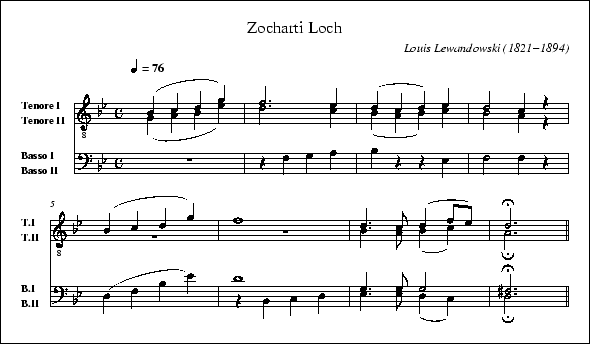
\includegraphics{wiki/_media/abc-standard-multivoice-80.png}}

\texttt{V:} can appear both in the body and the header. In the latter
case, \texttt{V:} is used exclusively to set voice properties. For
example, the \texttt{name} property in the example above, specifies
which label should be printed on the first staff of the voice in
question. Note that these properties may be also set or changed in the
\protect\hyperlink{tune_body_definition}{tune body}. The \texttt{V:}
properties are fully explained
\protect\hyperlink{voice_properties}{below}.

Please note that the exact grouping of voices on the staff or staves is
not specified by \texttt{V:} itself. This may be specified with the
\texttt{\%\%score}
\protect\hyperlink{stylesheet_directive_definition}{stylesheet
directive}. See \protect\hyperlink{voice_grouping}{voice grouping} for
details.

For playback, see
\protect\hyperlink{instrumentation_directives}{instrumentation
directives} for details of how to assign a General MIDI instrument to a
voice using a \texttt{\%\%MIDI}
\protect\hyperlink{stylesheet_directive_definition}{stylesheet
directive}.

Although it is not recommended, the
\protect\hyperlink{tune_body_definition}{tune body} of fragment
\texttt{X:1}, could also be notated this way:

\begin{verbatim}
X:2
T:Zocharti Loch
%...skipping rest of the header...
K:Gm
%               Start of tune body:
V:T1
 (B2c2 d2g2) | f6e2 | (d2c2 d2)e2 | d4 c2z2 |
 (B2c2 d2g2) | f8 | d3c (d2fe) | H d6 ||
V:T2
 (G2A2 B2e2) | d6c2 | (B2A2 B2)c2 | B4 A2z2 |
 z8 | z8 | B3A (B2c2) | H A6 ||
V:B1
 z8 | z2f2 g2a2 | b2z2 z2 e2 | f4 f2z2 |
 (d2f2 b2e'2) | d'8 | g3g  g4 | H^f6 ||
V:B2
 x8 | x8 | x8 | x8 |
 x8 | z2B2 c2d2 | e3e (d2c2) | H d6 ||
\end{verbatim}

In the example above, each \texttt{V:} label occurs only once, and the
complete part for that voice follows. The output of tune \texttt{X:2}
will be exactly the same as the output of tune \texttt{X:1}; the source
code of \texttt{X:1}, however, is much easier to read.

\hypertarget{voice_properties}{\subsubsection{7.1 Voice
properties}\label{voice_properties}}

\emph{VOLATILE:} See \protect\hyperlink{multiple_voices}{above}.

\texttt{V:} fields can contain voice specifiers such as name, clef, and
so on. For example,

\begin{verbatim}
V:T name="Tenor" clef=treble-8
\end{verbatim}

indicates that voice \texttt{T} will be drawn on a staff labelled
\texttt{Tenor}, using the treble clef with a small \texttt{8}
underneath. Player programs will transpose the notes by one octave.
Possible voice definitions include:

\begin{itemize}
\item
  \textbf{name=``voice name''} - the voice name is printed on the left
  of the first staff only. The characters \texttt{\textbackslash{}n}
  produce a newline in the output.
\item
  \textbf{subname=``voice subname''} - the voice subname is printed on
  the left of all staves but the first one.
\item
  \textbf{stem=up/down} - forces the note stem direction.
\item
  \textbf{clef=} - specifies a clef; see
  \protect\hyperlink{clefs_and_transposition}{clefs and transposition}
  for details.
\end{itemize}

The name specifier may be abbreviated to \texttt{nm=}. The subname
specifier may be abbreviated to \texttt{snm=}.

Applications may implement their own specifiers, but must gracefully
ignore specifiers they don't understand or implement. This is required
for portability of \protect\hyperlink{abc_file_definition}{abc files}
between applications.

\hypertarget{breaking_lines}{\subsubsection{7.2 Breaking
lines}\label{breaking_lines}}

\emph{VOLATILE:} See \protect\hyperlink{multiple_voices}{above}. In
particular the following may be relaxed with the introduction of a
control voice.

The rules for \protect\hyperlink{typesetting_line-breaks}{typesetting
line-breaks} in multi-voice \protect\hyperlink{abc_tune_definition}{abc
tunes} are the same as for single voice music although additionally a
line-break in one voice must be matched in the other voices. See the
example tune \protect\hyperlink{canzonettaabc}{Canzonetta.abc}.

\hypertarget{inline_fields}{\subsubsection{7.3 Inline
fields}\label{inline_fields}}

\emph{VOLATILE:} See \protect\hyperlink{multiple_voices}{above}.

To avoid ambiguity, \protect\hyperlink{inline_field_definition}{inline
fields} that specify music properties should be repeated in every voice
to which they apply.

\emph{Example:}

\begin{verbatim}
[V:1] C4|[M:3/4]CEG|Gce|
[V:2] E4|[M:3/4]G3 |E3 |
\end{verbatim}

\hypertarget{voice_overlay}{\subsubsection{7.4 Voice
overlay}\label{voice_overlay}}

\emph{VOLATILE:} See \protect\hyperlink{multiple_voices}{above}.

The \texttt{\&} operator may be used to temporarily overlay several
voices within one measure. Each \texttt{\&} operator sets the time point
of the music back by one bar line, and the notes which follow it form a
temporary voice in parallel with the preceding one. This may only be
used to add one complete bar's worth of music for each \texttt{\&}.

Example:

\begin{verbatim}
A2 | c d e f g  a  &\
     A A A A A  A  &\
     F E D C B, A, |]
\end{verbatim}

\href{/wiki/_detail/abc:standard:overlay1-80.png?id=abc\%3Astandard\%3Av2.1}{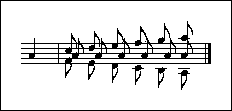
\includegraphics{wiki/_media/abc-standard-overlay1-80.png}}

Words in \texttt{w:} lines (and symbols in \texttt{s:} lines) are
matched to the corresponding notes as per the normal rules for lyric
alignment (see \protect\hyperlink{lyrics}{lyrics}), disregarding any
overlay in the accompanying
\protect\hyperlink{music_code_definition}{music code}.

\emph{Example:}

\begin{verbatim}
    g4 f4 | e6 e2 |
&& (d8    | c6) c2|
w: ha-la-| lu-yoh
+: lu-   |   -yoh
\end{verbatim}

\href{/wiki/_detail/abc:standard:overlay3-80.png?id=abc\%3Astandard\%3Av2.1}{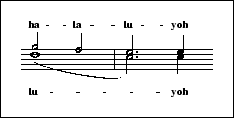
\includegraphics{wiki/_media/abc-standard-overlay3-80.png}}

This revokes the abc 2.0 usage of \texttt{\&} in \texttt{w:} and
\texttt{s:} lines, which is now
\protect\hyperlink{outdated_syntax}{deprecated} (see
\protect\hyperlink{disallowed_voice_overlay}{disallowed}).

\begin{center}\rule{0.5\linewidth}{\linethickness}\end{center}

\hypertarget{abc_data_format}{\subsection{8. Abc data
format}\label{abc_data_format}}

Each line in the file may end with white-space which will be ignored.
For the purpose of this standard, ASCII tab and space characters are
equivalent and are both included in the term `white-space'. Applications
must be able to interpret end-of-line markers in Unix
(\texttt{\textless{}LF\textgreater{}}), Windows/DOS
(\texttt{\textless{}CR\textgreater{}\textless{}LF\textgreater{}}), and
Macintosh style (\texttt{\textless{}CR\textgreater{}}) correctly.

\hypertarget{tune_body}{\subsubsection{8.1 Tune body}\label{tune_body}}

Within the \protect\hyperlink{tune_body_definition}{tune body}, all the
printable ASCII characters may be used for the
\protect\hyperlink{music_code_definition}{music code}. These are:

\begin{verbatim}
 !"#$%&'()*+,-./0123456789:;<=>?@
ABCDEFGHIJKLMNOPQRSTUVWXYZ[\]^_`
abcdefghijklmnopqrstuvwxyz{|}~
\end{verbatim}

Of these, the following characters are currently reserved:

\begin{verbatim}
# * ; ? @
\end{verbatim}

In future standards they may be used to extend the abc syntax.

To ensure forward compatibility, current software should ignore these
characters when they appear inside or between note groups, possibly
giving a warning. However, these characters may not be ignored when they
appear inside \protect\hyperlink{text_string_definition}{text strings}
or \protect\hyperlink{information_field_definition}{information fields}.

\emph{Example:}

\begin{verbatim}
@a !pp! #bc2/3* [K:C#] de?f "@this $2was difficult to parse?" y |**
\end{verbatim}

should be treated as:

\begin{verbatim}
a !pp! bc2/3 [K:C#] def "@this $2was difficult to parse?" y |
\end{verbatim}

\hypertarget{text_strings}{\subsubsection{8.2 Text
strings}\label{text_strings}}

\href{}{}Text written within an
\protect\hyperlink{abc_file_definition}{abc file}, either as part of an
\protect\hyperlink{information_field_definition}{information field}, an
\protect\hyperlink{annotations}{annotation} or as
\protect\hyperlink{free_text_definition}{free text} /
\protect\hyperlink{typeset_text_definition}{typeset text}, is known as a
\textbf{text string}, or more fully, an \textbf{abc text string}. (Note
that the abc standard version 2.0 referred to a
\protect\hyperlink{text_string_definition}{text string} as an \emph{abc
string}.)

Typically when there are several lines of text, each line forms a
separate \protect\hyperlink{text_string_definition}{text string},
although the distinction is not essential.

The contents of a text string may be written using any legal
\protect\hyperlink{charset_field}{character set}. The default character
set is \texttt{utf-8}, giving access to every Unicode character.

However, not all text editors support \texttt{utf-8} and so to avoid
portability problems when writing accented characters in text strings,
it also possible to use three other encoding options:

\begin{itemize}
\item
  \textbf{mnemonics} - for example, é can be represented by
  \texttt{\textbackslash{}\textquotesingle{}e}. These mnemonics are are
  based on TeX encodings and are always in the format
  \emph{backslash-mnemonic-letter}. They have been available since the
  earliest days of abc and are widely used in legacy abc files. They are
  generally easy to remember and easy to read, but are not comprehensive
  in terms of the possible accents they can represent.
\item
  \textbf{named html entities} - for example, é can be represented by
  \texttt{\&eacute;}. These encodings are not common in legacy abc files
  but are convenient for websites which use abc and generally easy to
  remember. However they are not particularly easy to read and are not
  fully comprehensive in terms of the possible accents they can
  represent.
\item
  \textbf{fixed width unicode} - for example, é can be represented by
  \texttt{\textbackslash{}u00e9} using the 16-bit unicode representation
  \texttt{00e9} (or \texttt{\textbackslash{}U000000e9} using 32-bit).
  These encodings are not common in legacy abc files and are not easy to
  read but give comprehensive access to all unicode characters.
\end{itemize}

All conforming abc typesetting software should support (understand and
be able to convert) the subset of accents and ligatures given in the
appendix, \protect\hyperlink{supported_accents_ligatures}{supported
accents \& ligatures}, together with the special characters and symbols
listed below.

A summary, with examples, is as follows:

\begin{longtable}[]{@{}lll@{}}
\toprule
Accent & Examples & Encodings\tabularnewline
\midrule
\endhead
grave & \texttt{À\ à\ è\ ò} &
\texttt{\textbackslash{}`A\ \textbackslash{}`a\ \textbackslash{}`e\ \textbackslash{}`o}\tabularnewline
acute & \texttt{Á\ á\ é\ ó} &
\texttt{\textbackslash{}\textquotesingle{}A\ \textbackslash{}\textquotesingle{}a\ \textbackslash{}\textquotesingle{}e\ \textbackslash{}\textquotesingle{}o}\tabularnewline
circumflex & \texttt{Â\ â\ ê\ ô} &
\texttt{\textbackslash{}\^{}A\ \textbackslash{}\^{}a\ \textbackslash{}\^{}e\ \textbackslash{}\^{}o}\tabularnewline
tilde & \texttt{Ã\ ã\ ñ\ õ} &
\texttt{\textbackslash{}\textasciitilde{}A\ \textbackslash{}\textasciitilde{}a\ \textbackslash{}\textasciitilde{}n\ \textbackslash{}\textasciitilde{}o}\tabularnewline
umlaut & \texttt{Ä\ ä\ ë\ ö} &
\texttt{\textbackslash{}"A\ \textbackslash{}"a\ \textbackslash{}"e\ \textbackslash{}"o}\tabularnewline
cedilla & \texttt{Ç\ ç} &
\texttt{\textbackslash{}cC\ \textbackslash{}cc}\tabularnewline
ring & \texttt{Å\ å} &
\texttt{\textbackslash{}AA\ \textbackslash{}aa}\tabularnewline
slash & \texttt{Ø\ ø} &
\texttt{\textbackslash{}/O\ \textbackslash{}/o}\tabularnewline
breve & \texttt{Ă\ ă\ Ĕ\ ĕ} &
\texttt{\textbackslash{}uA\ \textbackslash{}ua\ \textbackslash{}uE\ \textbackslash{}ue}\tabularnewline
caron & \texttt{Š\ š\ Ž\ ž} &
\texttt{\textbackslash{}vS\ \textbackslash{}vs\ \textbackslash{}vZ\ \textbackslash{}vz}\tabularnewline
double acute & \texttt{Ő\ ő\ Ű\ ű} &
\texttt{\textbackslash{}HO\ \textbackslash{}Ho\ \textbackslash{}HU\ \textbackslash{}Hu}\tabularnewline
ligatures & \texttt{ß\ Æ\ æ\ œ} &
\texttt{\textbackslash{}ss\ \textbackslash{}AE\ \textbackslash{}ae\ \textbackslash{}oe}\tabularnewline
\bottomrule
\end{longtable}

Programs that have difficulty typesetting accented letters may reduce
them to the base letter or, in the case of ligatures, the two base
letters ignoring the backslash.

\emph{Examples:} When reduced to the base letter,
\texttt{\textbackslash{}oA} becomes \texttt{A},
\texttt{\textbackslash{}"o} becomes \texttt{o},
\texttt{\textbackslash{}ss} becomes \texttt{ss},
\texttt{\textbackslash{}AE} becomes \texttt{AE}, etc.

For fixed width unicode, \texttt{\textbackslash{}u} or
\texttt{\textbackslash{}U} must be followed by 4 or 8 hexadecimal
characters respectively. Thus if any of the 4 characters after
\texttt{\textbackslash{}u} is not hexadecimal, then it is interpreted as
a breve.

\subparagraph{Special characters}\label{special_characters}

Characters that are meaningful in the context of a
\protect\hyperlink{text_string_definition}{text string} can be escaped
using a backslash as follows:

\begin{itemize}
\item
  type \texttt{\textbackslash{}\textbackslash{}} to get a backslash;
\item
  type \texttt{\textbackslash{}\%} to get a percent symbol that is not
  interpreted as the start of a
  \protect\hyperlink{comments_and_remarks}{comment};
\item
  type \texttt{\textbackslash{}\&} to get an ampersand that is not
  interpreted as the start of a named html entity (although an ampersand
  followed by white-space is interpreted as is - for example,
  \texttt{gin\ \&\ tonic} is OK, but \texttt{G\textbackslash{}\&T}
  requires the backslash);
\item
  type \texttt{\&quot;} or \texttt{\textbackslash{}u0022} to get double
  quote marks in an \protect\hyperlink{annotations}{annotation}
\end{itemize}

\hypertarget{special_symbols}{\subparagraph{Special
symbols}\label{special_symbols}}

The following symbols are also useful:

\begin{itemize}
\item
  type \texttt{\&copy;} or \texttt{\textbackslash{}u00a9} for the
  copyright symbol ©
\item
  type \texttt{\textbackslash{}u266d} for a flat symbol ♭
\item
  type \texttt{\textbackslash{}u266e} for a natural symbol ♮
\item
  type \texttt{\textbackslash{}u266f} for a sharp symbol ♯
\end{itemize}

\emph{VOLATILE:} Finally note that currently the specifiers
\texttt{\$1}, \texttt{\$2}, \texttt{\$3} and \texttt{\$4} can be used to
change the font within a \protect\hyperlink{text_string_definition}{text
string}. However, this feature is likely to change in future versions of
the standard - see \protect\hyperlink{font_directives}{font directives}
for more details.

\begin{center}\rule{0.5\linewidth}{\linethickness}\end{center}

\hypertarget{macros}{\subsection{9. Macros}\label{macros}}

This standard defines an \textbf{optional} system of macros which is
principally used to define the way in which ornament symbols such as the
tilde \texttt{\textasciitilde{}} are played (although it could be used
for many other purposes).

Software implementing these macros, should first expand the macros
defined in this section, and only afterwards apply any relevant
\texttt{U:} replacement (see
\protect\hyperlink{redefinable_symbols}{Redefinable symbols}).

When these macros are stored in an abc header file (see
\protect\hyperlink{include_field}{include field}), they may form a
powerful library.

There are two kinds of macro, called Static and Transposing.

\hypertarget{static_macros}{\subsubsection{9.1 Static
macros}\label{static_macros}}

You define a static macro by writing into the
\protect\hyperlink{tune_header_definition}{tune header} something like
this:

\begin{verbatim}
 m: ~G3 = G{A}G{F}G
\end{verbatim}

When you play the tune, the program searches the
\protect\hyperlink{tune_header_definition}{tune header} for macro
definitions, then does a search and replace on its internal copy of the
text before passing that to the parser which plays the tune. Every
occurence of \texttt{\textasciitilde{}G3} in the tune is replaced by
\texttt{G\{A\}G\{F\}G}, and that is what gets played. Only
\texttt{\textasciitilde{}G3} notes are affected,
\texttt{\textasciitilde{}G2}, \texttt{\textasciitilde{}g3},
\texttt{\textasciitilde{}F3} etc. are ignored.

You can put in as many macros as you want, and indeed, if you only use
static macros you will need to write a separate macro for each
combination of pitch and note-length. Here is an example:

\begin{verbatim}
X:50
T:Apples in Winter
S:Trad, arr. Paddy O'Brien
R:jig
m: ~g2 = {a}g{f}g
m: ~D2 = {E}D{C}D
M:6/8
K:D
G/2A/2|BEE dEE|BAG FGE|~D2D FDF|ABc ded|
BEE BAB|def ~g2 e|fdB AGF|GEE E2:|
d|efe edB|ege fdB|dec dAF|DFA def|
[1efe edB|def ~g2a|bgb afa|gee e2:|
[2edB def|gba ~g2e|fdB AGF|GEE E2||
\end{verbatim}

Here I have put in two static macros, since there are two different
notes in the tune marked with a tilde.

A static macro definition consists of four parts:

\begin{itemize}
\item
  the field identifier \texttt{m:}
\item
  the target string - e.g \texttt{\textasciitilde{}G3}
\item
  the equals sign
\item
  the replacement string - e.g. \texttt{G\{A\}G\{F\}G}
\end{itemize}

The target string can consist of any string up to 31 characters in
length, except that it may not include the letter `n', for reasons which
will become obvious later. You don't have to use the tilde, but of
course if you don't use a legal combination of abc, other programs will
not be able to play your tune.

The replacement string consists of any legal abc text up to 200
characters in length. It's up to you to ensure that the target and
replacement strings occupy the same time interval (the program does not
check this). Both the target and replacement strings may include spaces
if necessary, but leading and trailing spaces are stripped off so

\begin{verbatim}
m:~g2={a}g{f}g
\end{verbatim}

is perfectly OK, although less readable.

\hypertarget{transposing_macros}{\subsubsection{9.2 Transposing
macros}\label{transposing_macros}}

If your tune has ornaments on lots of different notes, and you want them
to all play with the same ornament pattern, you can use transposing
macros to achieve this. Transposing macros are written in exactly the
same way as static macros, except that the note symbol in the target
string is represented by `n' (meaning any note) and the note symbols in
the replacement string by other letters (h to z) which are interpreted
according to their position in the alphabet relative to n.

So, for example I could re-write the static macro
\texttt{m:\ \textasciitilde{}G3\ =\ G\{A\}G\{F\}G} as a transposing
macro \texttt{m:\ \textasciitilde{}n3\ =\ n\{o\}n\{m\}n}. When the
transposing macro is expanded, any note of the form
\texttt{\textasciitilde{}n3} will be replaced by the appropriate pattern
of notes. Notes of the form \texttt{\textasciitilde{}n2} (or other
lengths) will be ignored, so you will have to write separate transposing
macros for each note length.

Here's an example:

\begin{verbatim}
X:35
T:Down the Broom
S:Trad, arr. Paddy O'Brien
R:reel
M:C|
m: ~n2 = (3o/n/m/ n                % One macro does for all four rolls
K:ADor
EAAG~A2 Bd|eg~g2 egdc|BGGF GAGE|~D2B,D GABG|
EAAG ~A2 Bd|eg~g2 egdg|eg~g2 dgba|gedB BAA2:|
~a2ea agea|agbg agef|~g2dg Bgdg|gfga gede|
~a2 ea agea|agbg ageg|dg~g2 dgba|gedB BA A2:|
\end{verbatim}

A transposing macro definition consists of four parts:

\begin{itemize}
\item
  the field identifier \texttt{m:}
\item
  the target string - e.g \texttt{\textasciitilde{}n3}
\item
  the equals sign
\item
  the replacement string - e.g. \texttt{n\{o\}n\{m\}n}
\end{itemize}

The target string can consist of any string up to 31 characters in
length, except that it must conclude with the letter `n', followed by a
number which specifies the note length.

The replacement string consists of any legal abc text up to 200
characters in length, where note pitches are defined by the letters h -
z, the pitches being interpreted relative to that of the letter n. Once
again you should ensure that the time intervals match. You should not
use accidentals in transposing macros

\emph{Comment:} It is almost impossible to think of a way to transpose
\texttt{\textasciitilde{}=a3} or \texttt{\textasciitilde{}\^{}G2} which
will work correctly under all circumstances, so a static macro should be
used for cases like these.

\begin{center}\rule{0.5\linewidth}{\linethickness}\end{center}

\hypertarget{outdated_syntax}{\subsection{10. Outdated
syntax}\label{outdated_syntax}}

The abc standard contains a variety of outdated syntax that is no longer
recommended or, in some cases even supported, according to the following
definitions:

\begin{itemize}
\item
  \textbf{Deprecated} syntax is rules or constructs that have been
  outdated by newer syntax. Deprecated syntax must be supported by
  conforming abc software under strict interpretation but is not
  recommended for new transcriptions. Deprecated syntax may become
  obsolete in future versions of abc. Conforming abc software that
  encounters deprecated syntax should issue a warning when using strict
  interpretation (although it may offer the user the option to switch
  warnings off).
\item
  \textbf{Obsolete} syntax is rules or constructs for which there is no
  guarantee of support by conforming abc software. Obsolete syntax may
  be supported under loose interpretation but must not be used for new
  transcriptions. Conforming abc software that encounters obsolete
  syntax should issue a (preferably non-fatal) error message when using
  strict interpretation, or a warning when using loose interpretation
  (although it may offer the user the option to switch warnings off).
\item
  \textbf{Disallowed} syntax has the same definition as obsolete syntax,
  but has not gone through a formal process of deprecation.
\item
  \textbf{Outdated} syntax is the collective term for deprecated,
  obsolete and disallowed syntax.
\end{itemize}

Please see \url{http://www.ietf.org/rfc/rfc2119.txt} for formal
definitions of the key words MUST, MUST NOT, REQUIRED, SHALL, SHALL NOT,
SHOULD, SHOULD NOT, RECOMMENDED, MAY, and OPTIONAL in this context.

Outdated abc syntax is listed below so that users who come across it are
able to interpret (and preferably update) it according to the latest
standard.

\hypertarget{outdated_information_field_syntax}{\subsubsection{10.1
Outdated information field
syntax}\label{outdated_information_field_syntax}}

The \texttt{A:} \protect\hyperlink{aarea}{field} was originally used to
contain area information. In version 2.0 this was changed to contain the
name of the lyrics author. In version 2.1, to maintain backwards
compatibility, this has been changed back to area, but for clarity, the
\texttt{A:} field is \protect\hyperlink{outdated_syntax}{deprecated} -
area information can be stored in the \texttt{O:} field and a new field
\emph{(to be decided)} will be used for author information.

\emph{Comment:} Of the 160,000 tunes currently available in the
\href{http://abcnotation.com/search}{abcnotation.com tune search} 16,300
contain an \texttt{A:} field with 680 distinct values. Of these, only
around 10 contain author information rather than area (in some cases it
is difficult to tell).

An \texttt{E:} field was once used by \texttt{abc2mtex} to explicitly
control note spacing; this is no longer necessary with current
formatting algorithms and the \texttt{E:} field is now
\protect\hyperlink{outdated_syntax}{deprecated}.

The original usage of the \texttt{H:}
\protect\hyperlink{hhistory}{history} field, where the contents of the
history field is considered to continue over several lines until the
next field occurs, is now
\protect\hyperlink{outdated_syntax}{deprecated}.

The \texttt{Q:} \protect\hyperlink{qtempo}{tempo} field is still very
much in use, but earlier versions of the standard permitted two syntax
variants, now \protect\hyperlink{outdated_syntax}{deprecated}, which
specified how many unit note lengths to play per minute.

\emph{Examples:} Both examples mean ``play 120 unit note-lengths per
minute''.

\begin{verbatim}
Q:C=120
Q:120
\end{verbatim}

This is not very musical, and the usage is
\protect\hyperlink{outdated_syntax}{deprecated}. However, there are many
\protect\hyperlink{abc_file_definition}{abc files} which employ this
syntax and programs should accept it.

\hypertarget{outdated_dialects}{\subsubsection{10.2 Outdated
dialects}\label{outdated_dialects}}

\hypertarget{outdated_line-breaking}{\paragraph{10.2.1 Outdated
line-breaking}\label{outdated_line-breaking}}

The popular abc software abc2win introduced an exclamation mark
(\texttt{!}) as a way of forcing a
\protect\hyperlink{score_line-break_definition}{score line-break} and
this was adopted by abc 2.0, conflicting with the previous usage of
\texttt{!\ldots{}!} to delimit decorations.

The \texttt{!} is now \protect\hyperlink{outdated_syntax}{deprecated}
for \protect\hyperlink{score_line-break_definition}{score line-breaks}
although it is still available (even under
\protect\hyperlink{strict_interpretation}{strict interpretation}) for
legacy abc transcriptions by use of the "\texttt{I:linebreak\ !}"
directive - see \protect\hyperlink{line-breaking_dialects}{line-breaking
dialects}.

\hypertarget{outdated_decorations}{\paragraph{10.2.2 Outdated
decorations}\label{outdated_decorations}}

Abc standard 2.0 adopted \texttt{+\ldots{}+} syntax to indicate
decorations in place of \texttt{!\ldots{}!}. It never gained much
favour, however, and the latter is in much more common (see
\protect\hyperlink{decoration_dialects}{decoration dialects}).

Therefore, and since a non-conflicting mechanism has now been found to
allow \texttt{!} for line-breaking (see
\protect\hyperlink{line-breaking_dialects}{line-breaking dialects}), the
\texttt{+\ldots{}+} decoration syntax is now
\protect\hyperlink{outdated_syntax}{deprecated} in favour of
\texttt{!\ldots{}!}.

Nonetheless, the \texttt{+\ldots{}+} decoration syntax is still
available using the "\texttt{I:decoration\ +}" instruction (see
\protect\hyperlink{decoration_dialects}{decoration dialects}).

\hypertarget{outdated_chords}{\paragraph{10.2.3 Outdated
chords}\label{outdated_chords}}

Early versions of the abc standard used the \texttt{+} symbol to delimit
chords (in place of \texttt{{[}{]}} symbols). This usage is now
\protect\hyperlink{outdated_syntax}{deprecated} - see
\protect\hyperlink{chord_dialects}{chord dialects} for more details.

\hypertarget{outdated_continuations}{\subsubsection{10.3 Outdated
continuations}\label{outdated_continuations}}

From the earliest days of abc (in abc standard 1.0 through to abc
1.7.6), the backslash (\texttt{\textbackslash{}}) has been used to
suppress \protect\hyperlink{score_line-break_definition}{score
line-breaks} by placing it at the end of a line of
\protect\hyperlink{music_code_definition}{music code}. Thus,
effectively, it has acted as a continuation character, although with its
own special rules, in particular that it could act through
\protect\hyperlink{information_field_definition}{information fields} and
\protect\hyperlink{comment_definition}{comments}.

Abc 2.0 extended this usage to make \texttt{\textbackslash{}} a general
continuation character, which also allows continuation of
\protect\hyperlink{information_field_definition}{information fields} and
in particular the \texttt{w:} lyrics field (usually the only field which
actually requires a continuation in typical transcriptions).
Unfortunately, however, the rules of precedence were never well
established (should the \texttt{\textbackslash{}} be treated by a
pre-processor joining together continued lines and, if so, should
comments be removed before or after that happened?) and the usage was
never widely adopted, nor even well understood.

\emph{Comment:} Of the 160,000 tunes currently available in the
\href{http://abcnotation.com/search}{abcnotation.com tune search}, only
22 (0.01\%) use continuations for the \texttt{w:} field and only around
50 (0.03\%) use it for any other field; of these latter usages, almost
all are actually in error.

Furthermore, discussions during the development of abc 2.1 led to the
suggestion that a new character should be introduced to suppress
\protect\hyperlink{score_line-break_definition}{score line-breaks} - in
other words the \texttt{\textbackslash{}} (as described in abc 2.0) had
evolved far enough away from its initial definition so that another
character was required to replace what it had originally been designed
to do.

Consequently, in abc 2.1 the \texttt{\textbackslash{}} has been
reinstated to its original purpose of suppressing
\protect\hyperlink{score_line-break_definition}{score line-breaks} (see
\protect\hyperlink{typesetting_line-breaks}{typesetting line-breaks})
and its use a general continuation character is now
\protect\hyperlink{outdated_syntax}{disallowed} (see
\protect\hyperlink{continuation_of_input_lines}{continuation of input
lines} for the alternatives).

\hypertarget{outdated_directives}{\subsubsection{10.4 Outdated
directives}\label{outdated_directives}}

The \texttt{\%\%continueall\ true} directive is replaced by
"\texttt{I:linebreak\ !}" in abc 2.1 (see
\protect\hyperlink{typesetting_line-breaks}{typesetting line-breaks})
and \protect\hyperlink{outdated_syntax}{deprecated}.

The \texttt{\%\%abc-copyright} and \texttt{\%\%abc-edited-by} extended
information fields from section 3.3. of abc 2.0 have been
\protect\hyperlink{outdated_syntax}{deprecated} in favour of the
\protect\hyperlink{ztranscription}{Z: - transcription} field.

\emph{Comment:} Of the 131,000 files currently available in the
\href{http://abcnotation.com/search}{abcnotation.com tune search} only
32 use \texttt{\%\%abc-edited-by} and only 1 uses
\texttt{\%\%abc-copyright}.

\hypertarget{outdated_file_structure}{\subsubsection{10.5 Outdated file
structure}\label{outdated_file_structure}}

\hypertarget{outdated_tune_header_syntax}{\paragraph{10.5.1 Outdated
tune header syntax}\label{outdated_tune_header_syntax}}

Abc standard 2.0 included the rule that 'if the
\protect\hyperlink{abc_file_definition}{abc file} contains only one tune
the \texttt{X:} field may be dropped'. However, it was pointed out that
as a consequence, a user who pasted an additional tune into such a file
would get an error message from a tune which previously contained no
errors.

Despite considerable discussion on the abcusers mail list (see for
example the threads
\url{http://tech.groups.yahoo.com/group/abcusers/message/3950} and
\url{http://tech.groups.yahoo.com/group/abcusers/message/4113}) and, a
number of good suggestions, no consensus was reached. As a result the
above rule is \protect\hyperlink{outdated_syntax}{deprecated} in abc
2.1; a tune must start with a \texttt{X:} field followed by a
\texttt{T:} field.

However, this decision may be revisited in the future and the
specification relaxed.

\hypertarget{outdated_defaults}{\paragraph{10.5.2 Outdated
defaults}\label{outdated_defaults}}

In early versions of the abc standard, defaults could be set throughout
an \protect\hyperlink{abc_file_definition}{abc file}, using
\protect\hyperlink{information_field_definition}{information fields},
which applied to all subsequent tune. In other words, the
\protect\hyperlink{file_header_definition}{file header} could
effectively appear anywhere inside a file instead of just at the top.

This usage significantly complicates random access of the tunes in the
file, since the all the preceding contents of the file must be scanned
for default settings before a tune can be processed. As result this was
\protect\hyperlink{outdated_syntax}{deprecated} in abc 2.0 and is
\protect\hyperlink{outdated_syntax}{deprecated} in abc 2.1.

\hypertarget{outdated_lyrics_alignment}{\subsubsection{10.6 Outdated
lyrics alignment}\label{outdated_lyrics_alignment}}

Abc 2.1 introduced an extension to \protect\hyperlink{alignment}{lyrics
alignment} meaning that lyric lines (i.e. those using the \texttt{w:}
field) no longer need to follow immediately after the line of
\protect\hyperlink{music_code_definition}{music code} to which they are
attached, meaning that they can even be postponed to the end of the
\protect\hyperlink{tune_body_definition}{tune body}.

\emph{Examples:} The following two excerpts are equivalent in abc 2.1;
under abc 2.0 and previous versions of the standard, only the first
version would be legal. Note that there are 4
(\protect\hyperlink{numbering}{numbered}) verses and hence 4 \texttt{w:}
fields for each line of \protect\hyperlink{music_code_definition}{music
code}.

In the first excerpt the lyrics follow immediately after the line of
\protect\hyperlink{music_code_definition}{music code} to which they are
attached.

In the second excerpt, the lyrics are postponed to the end of the tune,
arguably aiding readability substantially and meaning that each verse is
contiguous. The \protect\hyperlink{comment_definition}{comment lines} in
the second excerpt (those lines beginning with \texttt{\%}) are added
for readability and are entirely optional.

\begin{verbatim}
D2DE G2GG|A2EE ED-D2|c2cc B2AG|
w:1\-~Si les ma-tins de gri-sail-le se tein-tent,*s'ils ont cou-leur en la
w:2\-~Si mo-ri-bonds sont les rois en ri-pail-le,*si leurs pri-sons sont des
w:3\-~Si mill' so-leils de mé-tal pren-nent voi-le,*dix mill' so-leils de cris-
w:4\-~Si mill' bri-gands à l'en-can font par-ta-ge,*dix mille en-fants des tor-
A2B^c d4|e2ee d2BA|G2EF GABc|
w:nuit qui s'é-teint, vien-dront d'o-pal's len-de-mains, re-vien-dront les siè-cles
w:ca-ges sans fond, vien-ne l'heur' des é-va-sions,******
w:\-tal font mer-veille vienn'nt des lu-eurs de ver-meil,******
w:\-rents font ar-gent, vien-nent des fleurs de sa-fran,******
\end{verbatim}

\begin{verbatim}
%
% music
%
D2DE G2GG|A2EE ED-D2|c2cc B2AG|
A2B^c d4|e2ee d2BA|G2EF GABc|
%
% lyrics
%
w:1\-~Si les ma-tins de gri-sail-le se tein-tent,*s'ils ont cou-leur en la
+:nuit qui s'é-teint, vien-dront d'o-pal's len-de-mains, re-vien-dront les siè-cles
%
w:2\-~Si mo-ri-bonds sont les rois en ri-pail-le,*si leurs pri-sons sont des
+:ca-ges sans fond, vien-ne l'heur' des é-va-sions,******
%
w:3\-~Si mill' so-leils de mé-tal pren-nent voi-le,*dix mill' so-leils de cris-
+:\-tal font mer-veille vienn'nt des lu-eurs de ver-meil,******
%
w:4\-~Si mill' bri-gands à l'en-can font par-ta-ge,*dix mille en-fants des tor-
+:\-rents font ar-gent, vien-nent des fleurs de sa-fran,******
\end{verbatim}

Unfortunately, however, this extension is not fully backwards compatible
with abc 2.0.

The difficulty arises when there is a line (or lines) of music code
without lyrics attached, followed by a line with lyrics attached.

\emph{Example:} In the following excerpt, using abc 2.0 the lyrics would
be aligned with the adjacent
\protect\hyperlink{music_code_definition}{music code}, i.e. with
\texttt{cdef}; using abc 2.1 they would be aligned at the start of the
tune (or voice), i.e. with \texttt{CDEF}.

\begin{verbatim}
CDEF|
FEDC|
cdef|]
w:these are lyr-ics
\end{verbatim}

The work around for users who have files with such usage is either to
avoid writing \texttt{\%abc-2.1} as the
\protect\hyperlink{abc_file_identification}{file identifier} or to add
an empty \texttt{w:} field after the final line of
\protect\hyperlink{music_code_definition}{music code} that should be
without lyrics.

\emph{Example:} The following excerpt should be treated the same way
(with regard to lyrics alignment) under abc 2.0 and abc 2.1. Under abc
2.1 the empty \texttt{w:} field means that the lyrics are aligned with
\texttt{cdef}.

\begin{verbatim}
CDEF|
FEDC|
w:
cdef|]
w:these are lyr-ics
\end{verbatim}

\hypertarget{other_outdated_syntax}{\subsubsection{10.7 Other outdated
syntax}\label{other_outdated_syntax}}

\hypertarget{disallowed_voice_overlay}{\paragraph{10.7.1 Disallowed
voice overlay}\label{disallowed_voice_overlay}}

Although the use of ampersand (\texttt{\&}) to overlay voices (as
introduced in abc 2.0) is still perfectly acceptable, this usage has
been \protect\hyperlink{outdated_syntax}{deprecated} within \texttt{w:}
lyric and \texttt{s:} symbol
\protect\hyperlink{information_field_definition}{information fields}.

The reason is that, as far as is known, this usage has never been
implemented in software and, furthermore, \texttt{\&} symbols are widely
used within \texttt{w:} fields in legacy abc files to indicate
ampersands.

Instead lyrics are matched to notes without regard to the voice overlay
- see \protect\hyperlink{voice_overlay}{voice overlay}.

\begin{center}\rule{0.5\linewidth}{\linethickness}\end{center}

\hypertarget{stylesheet_directives_and_pseudo-comments}{\subsection{11.
Stylesheet directives and
pseudo-comments}\label{stylesheet_directives_and_pseudo-comments}}

\hypertarget{introduction_to_directives}{\subsubsection{11.0
Introduction to directives}\label{introduction_to_directives}}

\hypertarget{disclaimer}{\paragraph{11.0.1
Disclaimer}\label{disclaimer}}

In the early days of abc, pseudo-comments (lines starting with
\texttt{\%\%}) were introduced as a means of adding software-specific
information and formatting instructions into
\protect\hyperlink{abc_file_definition}{abc files}; because they started
with a \texttt{\%} symbol software that didn't recognise them would
ignore them as a \protect\hyperlink{comment_definition}{comment}.

In a valiant effort, abc 2.0 made an attempt to standardise these
pseudo-comments with the introduction
\protect\hyperlink{stylesheet_directive_definition}{stylesheet
directives} and the abc stylesheet specification. This was described as
``not part of the ABC specification itself'' but as ``an additional
standard'' containing directives to control how the content and
structural information described by the abc code ``is to be actually
rendered, for example by a typesetting or player program''.

Unfortunately, however, there are a very large number of pseudo-comment
directives and not all of them are well-defined. Furthermore, some
directives, in particular the \protect\hyperlink{text_directives}{text
directives} and \protect\hyperlink{accidental_directives}{accidental
directives}, actually contain content and / or structural information
(as opposed to rendering instructions).

Abc 2.1 has stepped away from this approach somewhat.

The pseudo-comments are still very much accepted as a way for developers
to introduce experimental features and software-specific formatting
instructions. However, when a directive gains acceptance, either by
being implemented in more than one piece of software, or by its use in a
substantial body of tunes, the aim is that the usage will be
standardised and adopted in the standard and the \texttt{I:}
\protect\hyperlink{iinstruction}{instruction} form recommended in place
of the \texttt{\%\%} pseudo-comment form.

In particular, it is intended that abc 2.3 will address markup and
embedding and at that point a number of the text-based directives,
together with other widely accepted forms, will be formally
incorporated.

For the moment, section 11 is retained mostly unchanged from abc 2.0
(save for typo corrections) but, as a result of the foregoing, the whole
of section 11 and all stylesheet directives should regarded as
\emph{VOLATILE}.

\hypertarget{stylesheet_directives}{\paragraph{11.0.2 Stylesheet
directives}\label{stylesheet_directives}}

\href{}{}A \textbf{stylesheet directive} is a line that starts with
\texttt{\%\%}, followed by a directive that gives instructions to
typesetting or player programs.

\emph{Examples:}

\begin{verbatim}
%%papersize A4
%%newpage
%%setbarnb 10
\end{verbatim}

Alternatively, any
\protect\hyperlink{stylesheet_directive_definition}{stylesheet
directive} may be written as an \texttt{I:instruction} field although
this is not recommended for usages which have not been standardised
(i.e. it is not recommended for any directives described in section 11).

\emph{Examples:} Not recommended.

\begin{verbatim}
I:papersize A4
I:newpage
I:setbarnb 10
\end{verbatim}

\protect\hyperlink{inline_field_definition}{Inline field} notation may
be used to place a
\protect\hyperlink{stylesheet_directive_definition}{stylesheet
directive} in the middle of a line of music:

\emph{Example:}

\begin{verbatim}
CDEFG|[I:setbarnb 10]ABc
\end{verbatim}

If a program doesn't recognise a
\protect\hyperlink{stylesheet_directive_definition}{stylesheet
directive}, it should just ignore it.

It should be stressed that the
\protect\hyperlink{stylesheet_directive_definition}{stylesheet
directives} are not formally part of the abc standard itself.
Furthermore, the list of possible
\protect\hyperlink{stylesheet_directive_definition}{directives} is long
and not standardised. They are provided by a variety of programs for
specifying layout, text annotations, fonts, spacings, voice instruments,
transposition and other details.

Strictly speaking, abc applications don't have to conform to the same
set of \protect\hyperlink{stylesheet_directive_definition}{stylesheet
directives}. However, it is desirable that they do in order to make
\protect\hyperlink{abc_file_definition}{abc files} portable between
different computer systems.

\hypertarget{voice_grouping}{\subsubsection{11.1 Voice
grouping}\label{voice_grouping}}

\emph{VOLATILE:} This section is under review as part of the general
discussion about \protect\hyperlink{multiple_voices}{multiple voices}
for abc 2.2. See also the \protect\hyperlink{disclaimer}{section 11
disclaimer}.

Basic syntax:

\begin{verbatim}
%%score <voice-id1> <voice-id2> ... <voice-idn>
\end{verbatim}

The score directive specifies which voices should be printed in the
score and how they should be grouped on the staves.

Voices that are enclosed by parentheses \texttt{()} will go on one
staff. Together they form a voice group. A voice that is not enclosed by
parentheses forms a voice group on its own that will be printed on a
separate staff.

If voice groups are enclosed by curly braces \texttt{\{\}}, the
corresponding staves will be connected by a big curly brace printed in
front of the staves. Together they form a voice block. This format is
used especially for typesetting keyboard music.

If voice groups or braced voice blocks are enclosed by brackets
\texttt{{[}{]}}, the corresponding staves will be connected by a big
bracket printed in front of the staves. Together they form a voice
block.

If voice blocks or voice groups are separated from each other by a
\texttt{\textbar{}} character, continued bar lines will be drawn between
the associated staves.

Example:

\begin{verbatim}
%%score Solo  [(S A) (T B)]  {RH | (LH1 LH2)}
\end{verbatim}

If a single voice surrounded by two voice groups is preceded by a star
(\texttt{*}), the voice is marked to be floating. This means that the
voice won't be printed on it's own staff; rather the software should
automatically determine, for each note of the voice, whether it should
be printed on the preceding staff or on the following staff.

Software that does not support floating voices may simply print the
voice on the preceding staff, as if it were part of the preceding voice
group.

Examples:

\begin{verbatim}
%%score {RH *M| LH}
%%score {(RH1 RH2) *M| (LH1 LH2)}
\end{verbatim}

String parts in an orchestral work are usually bracketed together and
the top two (1st/2nd violins) then braced outside the bracket:

\begin{verbatim}
%%score [{Vln1 | Vln2} | Vla | Vc | DB]
\end{verbatim}

Any voices appearing in the
\protect\hyperlink{tune_body_definition}{tune body} will only be printed
if it is mentioned in the score directive.

When the score directive occurs within the
\protect\hyperlink{tune_body_definition}{tune body}, it resets the music
generator, so that voices may appear and disappear for some period of
time.

If no score directive is used, all voices that appear in the
\protect\hyperlink{tune_body_definition}{tune body} are printed on
separate staves.

See \protect\hyperlink{canzonettaabc}{Canzonetta.abc} for an extensive
example.

An alternative directive to \texttt{\%\%score} is \texttt{\%\%staves}.

Both \texttt{\%\%score} and \texttt{\%\%staves} directives accept the
same parameters, but measure bar indications work the opposite way.
Therefore, \texttt{\%\%staves\ {[}S\textbar{}A\textbar{}T\textbar{}B{]}}
is equivalent to \texttt{\%\%score\ {[}S\ A\ T\ B{]}} and means that
continued bar lines are not drawn between the associated staves, while
\texttt{\%\%staves\ {[}S\ A\ T\ B{]}} is equivalent to
\texttt{\%\%score\ {[}S\textbar{}A\textbar{}T\textbar{}B{]}} and means
that they are drawn.

\hypertarget{instrumentation_directives}{\subsubsection{11.2
Instrumentation directives}\label{instrumentation_directives}}

\emph{VOLATILE:} See the \protect\hyperlink{disclaimer}{section 11
disclaimer}.

\begin{verbatim}
%%MIDI voice [<ID>] [instrument=<integer> [bank=<integer>]] [mute]
\end{verbatim}

Assigns a MIDI instrument to the indicated abc voice. The MIDI
instruments are organized in banks of 128 instruments each. Both the
instruments and the banks are numbered starting from one.

The General MIDI (GM) standard defines a portable, numbered set of 128
instruments (numbered from 1-128) - see
\url{http://www.midi.org/techspecs/gm1sound.php}. The GM instruments can
be used by selecting bank one. Since the contents of the other MIDI
banks is platform dependent, it is highly recommended to only use the
first MIDI bank in tunes that are to be distributed.

The default bank number is 1 (one).

\emph{Example:} The following assigns GM instrument 59 (tuba) to voice
`Tb'.

\begin{verbatim}
%%MIDI voice Tb instrument=59
\end{verbatim}

If the voice ID is omitted, the instrument is assigned to the current
voice.

\emph{Example:}

\begin{verbatim}
M:C
L:1/8
Q:1/4=66
K:C
V:Rueckpos
%%MIDI voice instrument=53 bank=2
A3B    c2c2    |d2e2    de/f/P^c3/d/|d8    |z8           |
V:Organo
%%MIDI voice instrument=73 bank=2
z2E2-  E2AG    |F2E2    F2E2        |F6  F2|E2CD   E3F/G/|
\end{verbatim}

You can use the keyword \texttt{mute} to mute the specified voice.

Some abc players can automatically generate an accompaniment based on
the \protect\hyperlink{chord_symbols}{chord symbols} specified in the
melody line. To suggest a GM instrument for playing this accompaniment,
use the following directive:

\begin{verbatim}
%%MIDI chordprog 20 % Church organ
\end{verbatim}

\hypertarget{accidental_directives}{\subsubsection{11.3 Accidental
directives}\label{accidental_directives}}

\emph{VOLATILE:} This section is under active discussion. See also the
\protect\hyperlink{disclaimer}{section 11 disclaimer}.

\begin{verbatim}
%%propagate-accidentals not | octave | pitch
\end{verbatim}

When set to \texttt{not}, accidentals apply only to the note they're
attached to. When set to \texttt{octave}, accidentals also apply to all
the notes of the same pitch in the same octave up to the end of the bar.
When set to \texttt{pitch}, accidentals also apply to all the notes of
the same pitch in all octaves up to the end of the bar.

The default value is \texttt{pitch}.

\begin{verbatim}
%%writeout-accidentals none | added | all
\end{verbatim}

When set to \texttt{none}, modifying or explicit accidentals that appear
in the key signature field (\texttt{K:}) are printed in the key
signature. When set to \texttt{added}, only the accidentals belonging to
the mode indicated in the \texttt{K:} field, are printed in the key
signature. Modifying or explicit accidentals are printed in front of the
notes to which they apply. When set to \texttt{all}, both the
accidentals belonging to the mode and possible modifying or explicit
accidentals are printed in front of the notes to which they apply; no
key signature will be printed.

The default value is \texttt{none}.

\hypertarget{formatting_directives}{\subsubsection{11.4 Formatting
directives}\label{formatting_directives}}

\emph{VOLATILE:} See the \protect\hyperlink{disclaimer}{section 11
disclaimer}.

Typesetting programs should accept the set of directives in the next
sections. The parameter of a directive can be a
\protect\hyperlink{text_string_definition}{text string}, a logical value
\texttt{true} or \texttt{false}, an integer number, a number with
decimals (just `number' in the following), or a unit of length. Units
can be expressed in cm, in, and pt (points, 1/72 inch).

The following directives should be self-explanatory.

\hypertarget{page_format_directives}{\paragraph{11.4.1 Page format
directives}\label{page_format_directives}}

\emph{VOLATILE:} See the \protect\hyperlink{disclaimer}{section 11
disclaimer}.

\begin{verbatim}
%%pageheight       <length>
%%pagewidth        <length>
%%topmargin        <length>
%%botmargin        <length>
%%leftmargin       <length>
%%rightmargin      <length>
%%indent           <length>
%%landscape        <logical>
\end{verbatim}

\hypertarget{font_directives}{\paragraph{11.4.2 Font
directives}\label{font_directives}}

\emph{VOLATILE:} Font directives are due to be considered in abc 2.3 -
see the \protect\hyperlink{disclaimer}{section 11 disclaimer}.

PostScript and PDF are the standard file formats for distributing
printable material. For portability reasons, typesetters will use the
PostScript font names. The size parameter should be an integer, but is
optional.

\begin{verbatim}
%%titlefont        <font name>  <size>
%%subtitlefont     <font name>  <size>
%%composerfont     <font name>  <size>
%%partsfont        <font name>  <size>
%%tempofont        <font name>  <size>
%%gchordfont       <font name>  <size> % for chords symbols
%%annotationfont   <font name>  <size> % for "^..." annotations
%%infofont         <font name>  <size>
%%textfont         <font name>  <size>
%%vocalfont        <font name>  <size> % for w:
%%wordsfont        <font name>  <size> % for W:
\end{verbatim}

The specifiers \texttt{\$1}, \texttt{\$2}, \texttt{\$3} and \texttt{\$4}
can be used to change the font within a
\protect\hyperlink{text_string_definition}{text string}. The font to be
used can be specified with the \texttt{\%\%setfont-n} directives.
\texttt{\$0} resets the font to its default value. \texttt{\$\$} gives
an actual dollar sign.

\begin{verbatim}
%%setfont-1        <font name>  <size>
%%setfont-2        <font name>  <size>
%%setfont-3        <font name>  <size>
%%setfont-4        <font name>  <size>
\end{verbatim}

\hypertarget{space_directives}{\paragraph{11.4.3 Space
directives}\label{space_directives}}

\emph{VOLATILE:} See the \protect\hyperlink{disclaimer}{section 11
disclaimer}.

\begin{verbatim}
%%topspace         <length>
%%titlespace       <length>
%%subtitlespace    <length>
%%composerspace    <length>
%%musicspace       <length> % between composer and 1st staff
%%partsspace       <length>
%%vocalspace       <length>
%%wordsspace       <length>
%%textspace        <length>
%%infospace        <length>
%%staffsep         <length> % between systems
%%sysstaffsep      <length> % between staves in the same system
%%barsperstaff     <integer>
%%parskipfac       <number> % space between parts
%%lineskipfac      <number> % space between lines of text
%%stretchstaff     <logical>
%%stretchlast      <logical>
%%maxshrink        <number> % shrinking notes
%%scale            <number>
\end{verbatim}

\hypertarget{measure_directives}{\paragraph{11.4.4 Measure
directives}\label{measure_directives}}

\emph{VOLATILE:} See the \protect\hyperlink{disclaimer}{section 11
disclaimer}.

\begin{verbatim}
%%measurefirst     <integer> % number of first measure
%%barnumbers       <integer> % bar numbers every 'n' measures
%%measurenb        <integer> % same as %%barnumbers
%%measurebox       <logical>
%%setbarnb         <integer> % set measure number
\end{verbatim}

\hypertarget{text_directives}{\paragraph{11.4.5 Text
directives}\label{text_directives}}

\emph{VOLATILE:} Text directives are due to be considered in abc 2.3 -
see the \protect\hyperlink{disclaimer}{section 11 disclaimer}.

The following directives can be used for inserting
\protect\hyperlink{typeset_text_definition}{typeset text} within an
\protect\hyperlink{abc_file_definition}{abc file}.

\begin{verbatim}
%%text             <text string>
%%center           <text string>
%%begintext
%%...              <text string>
%%endtext
\end{verbatim}

Notes:

\begin{itemize}
\item
  \texttt{\%\%text} prints the following text, treated as a
  \protect\hyperlink{text_string_definition}{text string}.
\item
  \texttt{\%\%center} prints the following text, treated as a
  \protect\hyperlink{text_string_definition}{text string} and centred.
\item
  \texttt{\%\%begintext} and \texttt{\%\%endtext} mark a section of
  lines, each of which start with \texttt{\%\%}, followed by some text.
  It is an alternative to several \texttt{\%\%text} lines.
  {[}\emph{Important note:} some
  \protect\hyperlink{abc_extensions}{extensions} offered by abc software
  programs relax the rule that each line between \texttt{\%\%begintext}
  and \texttt{\%\%endtext} must start with \texttt{\%\%}. Whilst this
  should not cause problems for
  \protect\hyperlink{typeset_text_definition}{typeset text} between
  tunes, \protect\hyperlink{typeset_text_definition}{typeset text}
  within a \protect\hyperlink{tune_header_definition}{tune header} or
  \protect\hyperlink{tune_body_definition}{tune body} should respect
  this rule and, in particular, must not introduce blank lines.{]}
\end{itemize}

See \protect\hyperlink{further_information_about_directives}{further
information about directives} for more details and to find out about
additional parameters for these directives.

\emph{Recommendation for users:} If you are using text directives for
tune-specific information, consider instead using one of the
\protect\hyperlink{bdfsbackground_information}{background information
fields} together with a \texttt{\%\%writefields} directive (see
\protect\hyperlink{information_directives}{information directives}) so
that the information can correctly identified by databasing software.

\hypertarget{information_directives}{\paragraph{11.4.6 Information
directives}\label{information_directives}}

\emph{VOLATILE:} The \texttt{\%\%writefields} directive and its
formatting options are likely to be enhanced when markup is considered
in abc 2.3. See also the \protect\hyperlink{disclaimer}{section 11
disclaimer}.

\begin{verbatim}
%%writefields <list of field identifiers> [<logical>]
\end{verbatim}

The \texttt{\%\%writefields} directive allows users to choose which
string-type \protect\hyperlink{information_field_definition}{information
fields} appear in the printed score (see the
\protect\hyperlink{information_fields}{information fields} table for a
list of string-type fields). It is followed by a list of field
identifiers and, optionally, the logical value \texttt{true} or
\texttt{false}. If the logical value is missing it is taken as
\texttt{true}.

The \texttt{\%\%writefields} directive also applies to certain
instruction fields - namely \texttt{X:reference\ number},
\texttt{P:parts} and \texttt{Q:tempo}.

The default is "\texttt{\%\%writefields\ TCOPQwW}" meaning that the
title (T), composer (C), origin (O), parts (P), tempo (Q), aligned words
(w) and other words (W) are printed out by default (see
\protect\hyperlink{typesetting_information_fields}{typesetting
information fields} for how these should be typeset). Each subseqent
\texttt{\%\%writefields} directive combines with this list, rather than
overriding it.

\emph{Examples:}

\begin{verbatim}
%%writefields O false         % the O field is not printed out - other defaults remain
%%writefields X               % the X: field is printed out
%%writefields BCDFGHNORSTWwXZ % all string-type fields are printed out
\end{verbatim}

Typesetting software conforming to abc 2.1 may format the information
strings in any way it chooses.

\emph{Comment:} The \texttt{\%\%writefields} directive can be used in
place of a number of directives introduced in abc 2.0:

\begin{itemize}
\item
  "\texttt{\%\%writefields\ X}" can be used as an alternative to
  "\texttt{\%\%withxrefs}"
\item
  "\texttt{\%\%writefields\ Ww\ false}" can be used as an alternative
  to"\texttt{\%\%musiconly}"
\item
  "\texttt{\%\%writefields}" is a partial alternative to
  "\texttt{\%\%writehistory}" and "\texttt{\%\%infoname}"
\end{itemize}

See \protect\hyperlink{further_information_about_directives}{further
information about directives} for more details of the 2.0 alternatives.

\hypertarget{separation_directives}{\paragraph{11.4.7 Separation
directives}\label{separation_directives}}

\emph{VOLATILE:} See the \protect\hyperlink{disclaimer}{section 11
disclaimer}.

\begin{verbatim}
%%sep     % draw a horizontal separator, i.e. a line
%%vskip   % insert some vertical space
%%newpage % start a new page
\end{verbatim}

See \protect\hyperlink{further_information_about_directives}{further
information about directives} for more details and to find out about
additional parameters for these directives.

\hypertarget{miscellaneous_directives}{\paragraph{11.4.8 Miscellaneous
directives}\label{miscellaneous_directives}}

\emph{VOLATILE:} See the \protect\hyperlink{disclaimer}{section 11
disclaimer}.

\begin{verbatim}
%%exprabove        <logical>
%%exprbelow        <logical>
%%graceslurs       <logical> % grace notes slur to main note
%%infoline         <logical> % rhythm and origin on the same line
%%oneperpage       <logical>
%%vocalabove       <logical>
%%freegchord       <logical> % print '#', 'b' and '=' as they are
%%printtempo       <logical>
\end{verbatim}

The default value for these directives is false.

\hypertarget{application_specific_directives}{\subsubsection{11.5
Application specific directives}\label{application_specific_directives}}

Applications may introduce their own directives. These directives should
start with the name of the application, followed a colon, folowed by the
name of the directive.

\emph{Example:}

\begin{verbatim}
%%noteedit:fontcolor blue
\end{verbatim}

\hypertarget{further_information_about_directives}{\subsubsection{11.6
Further information about
directives}\label{further_information_about_directives}}

Since \protect\hyperlink{stylesheet_directive_definition}{stylesheet
directives} are not formally part of the abc standard, only a subset is
included here. For additional directives and further information about
those listed here, see the user manuals for programs that implement
them, in particular:

\begin{itemize}
\item
  the \texttt{format.txt} file included with
  \href{http://moinejf.free.fr/}{abcm2ps}
\item
  the \texttt{abcguide.txt} file included with
  \href{http://abc.sourceforge.net/abcMIDI/}{abcMIDI}
\item
  the \texttt{abctab2ps}
  \href{http://www.lautengesellschaft.de/cdmm/userguide/userguide.html}{User's
  guide}
\end{itemize}

\begin{center}\rule{0.5\linewidth}{\linethickness}\end{center}

\hypertarget{dialects_strict_loose_interpretation_and_backwards_compatibility}{\subsection{12.
Dialects, strict / loose interpretation and backwards
compatibility}\label{dialects_strict_loose_interpretation_and_backwards_compatibility}}

Unfortunately a number of dialects of abc have arisen over the years,
partly due to differences in implementation, together with unfinished
drafts of the abc standard and ambiguities within it.

Version 2.1 of the standard aims to address this fragmentation of abc
notation with a robust, but tolerant approach that should accommodate as
many users as possible for several years to come and, as far as
possible, restore backwards compatibility.

There are three main approaches:

\begin{itemize}
\item
  the introduction of new \texttt{I:} directives to allow for
  preferences in dialects;
\item
  the concepts of strict and loose interpretation of the standard
  (together with recommendations to software developers for dealing with
  loose interpretations);
\item
  statistically-based decisions about default settings.
\end{itemize}

The aim is that, even under strict interpretation, most current dialects
are still available via the new \texttt{I:} directives.

\emph{Comment:} Dialects not available under strict interpretation are
those where one symbol is used for two different purposes - for example,
a \texttt{!} symbol used to denote both line-breaks and decorations;
fortunately, of the 160,000 tunes currently available in the
\href{http://abcnotation.com/search}{abcnotation.com tune search} only
around 60 (0.04\%) employ this usage.

\hypertarget{dialect_differences}{\subsubsection{12.1 Dialect
differences}\label{dialect_differences}}

The main differences that have arisen are line-breaks, decoration
delimiters and chord delimiters.

\hypertarget{line-breaking_dialects}{\paragraph{12.1.1 Line-breaking
dialects}\label{line-breaking_dialects}}

By default, a (forced)
\protect\hyperlink{score_line-break_definition}{score line-break} is
typeset by using a \protect\hyperlink{code_line-break_definition}{code
line-break} - see
\protect\hyperlink{typesetting_line-breaks}{typesetting line-breaks}.

In the past the \texttt{!} symbol has instead been used to indicate
\protect\hyperlink{score_line-break_definition}{score line-breaks} -
this symbol is now used to denote decorations.

\emph{Comment:} The \texttt{!} symbol was introduced by abc2win, a very
popular program in its time, although now moribund. Of the 160,000 tunes
currently available in the
\href{http://abcnotation.com/search}{abcnotation.com tune search}, only
around 1,600 (10\%) use the ! symbol to denote line-breaks.

Although the use of the \texttt{!} symbol for line-breaking is now
\protect\hyperlink{outdated_syntax}{deprecated} (see
\protect\hyperlink{outdated_line-breaking}{outdated line-breaking}),
users who wish to continue using the \texttt{!} symbol for line-breaking
merely need to include the "\texttt{I:linebreak\ !}" directive, either
in the \protect\hyperlink{file_header_definition}{file header} or
individually tune by tune - see
\protect\hyperlink{typesetting_line-breaks}{typesetting line-breaks}.

\emph{Example:} The following abc code would result in two lines of
music.

\begin{verbatim}
I:linebreak !
K:G
ABC DEF|!FED ABC|]
\end{verbatim}

Finally a new line-breaking symbol, \texttt{\$}, has been introduced as
an alternative to using
\protect\hyperlink{code_line-break_definition}{code line-breaks}.

\emph{Comment:} The \texttt{\$} symbol is effectively a replacement for
\texttt{!}. It is aimed at those users who want \texttt{!} as the
decoration delimiter but who prefer to use
\protect\hyperlink{code_line-break_definition}{code line-breaks} without
generating corresponding
\protect\hyperlink{score_line-break_definition}{score line-breaks}.

\hypertarget{decoration_dialects}{\paragraph{12.1.2 Decoration
dialects}\label{decoration_dialects}}

Decorations are delimited using the \texttt{!} symbol - see
\protect\hyperlink{decorations}{decorations}.

In the past the \texttt{+} symbol has instead been used to denote
decorations - this symbol is now
\protect\hyperlink{outdated_syntax}{deprecated} for decorations.

\emph{Comment:} Decorations were first introduced in draft standard
1.7.6 (which was never formally adopted) with the \texttt{!} symbol. In
abc 2.0 (adopted briefly whilst discussions about abc 2.1 were taking
place) this was changed to the \texttt{+} symbol. Neither are in
widespread use, but the \texttt{!} symbol is much more common - of the
160,000 tunes currently available in the
\href{http://abcnotation.com/search}{abcnotation.com tune search}, only
around 100 (0.07\%) use the \texttt{+} symbol to delimit decorations,
whereas around 1,350 (0.85\%) use the \texttt{!} symbol.

Users who wish to continue using the \texttt{+} symbol for decorations
merely need to include the "\texttt{I:decoration\ +}" directive, either
in the \protect\hyperlink{file_header_definition}{file header} or
individually tune by tune - see
\protect\hyperlink{decorations}{decorations}. All \texttt{+\ldots{}+}
decorations will then be treated as if they were the corresponding
\texttt{!\ldots{}!} decoration and any \texttt{!\ldots{}!} decorations
will generate an error message.

Note that the "\texttt{I:decoration\ +}" directive is automatically
invoked by the "\texttt{I:linebreak\ !}" directive. Also note that the
\texttt{!+!} decoration has no \texttt{+} equivalent - \texttt{+plus+}
should be used instead.

\emph{Recommendation for users:} Given the very small uptake of the
\texttt{+} symbol for decorations, "\texttt{I:decoration\ +}" directive
is not recommended. However, it is retained for users who wish to use
the \texttt{!} symbol for line-breaking in legacy
\protect\hyperlink{abc_file_definition}{abc files}.

For completeness the "\texttt{I:decoration\ !}", the default setting, is
also available to allow individual tunes to use \texttt{!\ldots{}!}
decorations in a file where "\texttt{I:decoration\ +}" is set in the
\protect\hyperlink{file_header_definition}{file header}.

\hypertarget{chord_dialects}{\paragraph{12.1.3 Chord
dialects}\label{chord_dialects}}

Chords are delimited using \texttt{{[}{]}} symbols - see
\protect\hyperlink{chords_and_unisons}{chords and unisons}.

In the past the \texttt{+} symbol has instead been used to delimit
chords - this symbol is no longer in use for chords.

\emph{Comment:} In early versions of the abc standard (1.2 to 1.5),
chords were delimited with \texttt{+} symbols. However, this made it
hard to see where one chord ended and another began and the chord
delimiters were changed to \texttt{{[}{]}} in 1.6 (November 1996). Of
the 160,000 tunes currently available in the
\href{http://abcnotation.com/search}{abcnotation.com tune search}, only
around 420 (0.25\%) use the \texttt{+} symbol to delimit chords. Given
the small uptake and the successful introduction of the \texttt{{[}{]}}
symbols, there is no \texttt{I:} directive available which allows the
use of \texttt{+} symbols and this usage is now
\protect\hyperlink{outdated_syntax}{obsolete}.

\hypertarget{loose_interpretation}{\subsubsection{12.2 Loose
interpretation}\label{loose_interpretation}}

\emph{Comment:} There are around 160,000 tunes currently available in
the \href{http://abcnotation.com/search}{abcnotation.com tune search} -
loose interpretation of the abc standard maintains backwards
compatibility without any changes required for this huge and valuable
resource.

Any \protect\hyperlink{abc_file_definition}{abc file} without a version
number, or with a version number of 2.0 or less (see
\protect\hyperlink{abc_file_identification}{abc file identification} and
\protect\hyperlink{version_field}{version field}), should be interpreted
loosely. Developers should do their best to provide programs that
understand legacy \protect\hyperlink{abc_file_definition}{abc files},
but users should be aware that loose interpretations may different from
one abc program to another.

\emph{Recommendation for users:} Try to avoid loose interpretation if
possible; loose interpretation means that if you pass abc notated tunes
on to friends, or post them on the web, they may not appear as you
hoped.

\emph{Recommendation 1 for developers:} Do your best! The most difficult
tunes to deal with are those which use the same symbol for two different
purposes - in particular the ! symbol for both decorations and
line-breaking. Here is an algorithm for helping to deal with
\texttt{!decoration!} syntax and \texttt{!} line-breaks in the same
tune:

When encountering a !, scan forward. If you find another ! before
encountering any of \texttt{\textbar{}{[}:{]}}, a space, or the end of a
line, then you have a decoration, otherwise it is a line-break.

\emph{Recommendation 2 for developers:} Although moving towards strict
interpretations should make life easier for everybody (developers and
users alike), you should allow users to switch easily between strict and
loose interpretation, perhaps via a command line switch or a GUI
check-box. For example, a user who imports an old
\protect\hyperlink{abc_file_definition}{abc file} may wish to see how it
would be interpreted strictly, perhaps to establish how many strict
errors need fixing.

\hypertarget{strict_interpretation}{\subsubsection{12.3 Strict
interpretation}\label{strict_interpretation}}

Any \protect\hyperlink{abc_file_definition}{abc file} with an abc
version number greater than or equal to 2.1 (see
\protect\hyperlink{abc_file_identification}{abc file identification} and
\protect\hyperlink{version_field}{version field}) should be interpreted
strictly, with errors indicated to the user as such.

\begin{center}\rule{0.5\linewidth}{\linethickness}\end{center}

\hypertarget{sample_abc_tunes}{\subsection{13. Sample abc
tunes}\label{sample_abc_tunes}}

\hypertarget{englishabc}{\subsubsection{13.1
English.abc}\label{englishabc}}

\begin{verbatim}
%abc-2.1
H:This file contains some example English tunes
% note that the comments (like this one) are to highlight usages
%  and would not normally be included in such detail
O:England             % the origin of all tunes is England

X:1                   % tune no 1
T:Dusty Miller, The   % title
T:Binny's Jig         % an alternative title
C:Trad.               % traditional
R:DH                  % double hornpipe
M:3/4                 % meter
K:G                   % key
B>cd BAG|FA Ac BA|B>cd BAG|DG GB AG:|
Bdd gfg|aA Ac BA|Bdd gfa|gG GB AG:|
BG G/2G/2G BG|FA Ac BA|BG G/2G/2G BG|DG GB AG:|
W:Hey, the dusty miller, and his dusty coat;
W:He will win a shilling, or he spend a groat.
W:Dusty was the coat, dusty was the colour;
W:Dusty was the kiss, that I got frae the miller.

X:2
T:Old Sir Simon the King
C:Trad.
S:Offord MSS          % from Offord manuscript
N:see also Playford   % reference note
M:9/8
R:SJ                  % slip jig
N:originally in C     % transcription note
K:G
D|GFG GAG G2D|GFG GAG F2D|EFE EFE EFG|A2G F2E D2:|
D|GAG GAB d2D|GAG GAB c2D|[1 EFE EFE EFG|A2G F2E D2:|\ % no line-break in score
M:12/8                % change of meter
[2 E2E EFE E2E EFG|\  % no line-break in score
M:9/8                 % change of meter
A2G F2E D2|]

X:3
T:William and Nancy
T:New Mown Hay
T:Legacy, The
C:Trad.
O:England; Gloucs; Bledington % place of origin
B:Sussex Tune Book            % can be found in these books
B:Mally's Cotswold Morris vol.1 2
D:Morris On                   % can be heard on this record
P:(AB)2(AC)2A                 % play the parts in this order
M:6/8
K:G                        
[P:A] D|"G"G2G GBd|"C"e2e "G"dBG|"D7"A2d "G"BAG|"C"E2"D7"F "G"G2:|
[P:B] d|"G"e2d B2d|"C"gfe "G"d2d| "G"e2d    B2d|"C"gfe    "D7"d2c|
        "G"B2B Bcd|"C"e2e "G"dBG|"D7"A2d "G"BAG|"C"E2"D7"F "G"G2:|
% changes of meter, using inline fields
[T:Slows][M:4/4][L:1/4][P:C]"G"d2|"C"e2 "G"d2|B2 d2|"Em"gf "A7"e2|"D7"d2 "G"d2|\
       "C"e2 "G"d2|[M:3/8][L:1/8] "G"B2 d |[M:6/8] "C"gfe "D7"d2c|
        "G"B2B Bcd|"C"e2e "G"dBG|"D7"A2d "G"BAG|"C"E2"D7"F "G"G2:|
\end{verbatim}

\hypertarget{strspysabc}{\subsubsection{13.2
Strspys.abc}\label{strspysabc}}

\begin{verbatim}
%abc-2.1
M:4/4
O:Scottish
R:Strathspey

X:1
T:A. A. Cameron's
K:D
e<A A2 B>G d>B|e<A A2 d>g (3fed|e<A A2 B>G d>B|B<G G>B d>g (3fed:|
B<e e>f g>e a>f|B<e e>f g>e (3fed|B<e e>f g>e a>f|d<B G>B d>g (3fed:|

X:2
T:Atholl Brose
% in this example, which reproduces Highland Bagpipe gracing,
%  the large number of grace notes mean that it is more convenient to be specific about
%  score line-breaks (using the $ symbol), rather than using code line breaks to indicate them
I:linebreak $
K:D
{gcd}c<{e}A {gAGAG}A2 {gef}e>A {gAGAG}Ad|
{gcd}c<{e}A {gAGAG}A>e {ag}a>f {gef}e>d|
{gcd}c<{e}A {gAGAG}A2 {gef}e>A {gAGAG}Ad|
{g}c/d/e {g}G>{d}B {gf}gG {dc}d>B:|$
{g}c<e {gf}g>e {ag}a>e {gf}g>e|
{g}c<e {gf}g>e {ag}a2 {GdG}a>d|
{g}c<e {gf}g>e {ag}a>e {gf}g>f|
{gef}e>d {gf}g>d {gBd}B<{e}G {dc}d>B|
{g}c<e {gf}g>e {ag}a>e {gf}g>e|
{g}c<e {gf}g>e {ag}a2 {GdG}ad|
{g}c<{GdG}e {gf}ga {f}g>e {g}f>d|
{g}e/f/g {Gdc}d>c {gBd}B<{e}G {dc}d2|]
\end{verbatim}

\hypertarget{reelsabc}{\subsubsection{13.3 Reels.abc}\label{reelsabc}}

\begin{verbatim}
%abc-2.1
M:4/4
O:Irish
R:Reel

X:1
T:Untitled Reel
C:Trad.
K:D
eg|a2ab ageg|agbg agef|g2g2 fgag|f2d2 d2:|\
ed|cecA B2ed|cAcA E2ed|cecA B2ed|c2A2 A2:|
K:G
AB|cdec BcdB|ABAF GFE2|cdec BcdB|c2A2 A2:|

X:2
T:Kitchen Girl
C:Trad.
K:D
[c4a4] [B4g4]|efed c2cd|e2f2 gaba|g2e2 e2fg|
a4 g4|efed cdef|g2d2 efed|c2A2 A4:|
K:G
ABcA BAGB|ABAG EDEG|A2AB c2d2|e3f edcB|ABcA BAGB|
ABAG EGAB|cBAc BAG2|A4 A4:|
\end{verbatim}

\hypertarget{canzonettaabc}{\subsubsection{13.4
Canzonetta.abc}\label{canzonettaabc}}

\begin{verbatim}
%abc-2.1
%%pagewidth      21cm
%%pageheight     29.7cm
%%topspace       0.5cm
%%topmargin      1cm
%%botmargin      0cm
%%leftmargin     1cm
%%rightmargin    1cm
%%titlespace     0cm
%%titlefont      Times-Bold 32
%%subtitlefont   Times-Bold 24
%%composerfont   Times 16
%%vocalfont      Times-Roman 14
%%staffsep       60pt
%%sysstaffsep    20pt
%%musicspace     1cm
%%vocalspace     5pt
%%measurenb      0
%%barsperstaff   5
%%scale          0.7
X: 1
T: Canzonetta a tre voci
C: Claudio Monteverdi (1567-1643)
M: C
L: 1/4
Q: "Andante mosso" 1/4 = 110
%%score [1 2 3]
V: 1 clef=treble name="Soprano"sname="A"
V: 2 clef=treble name="Alto"   sname="T"
V: 3 clef=bass middle=d name="Tenor"  sname="B"
%%MIDI program 1 75 % recorder
%%MIDI program 2 75
%%MIDI program 3 75
K: Eb
% 1 - 4
[V: 1] |:z4  |z4  |f2ec         |_ddcc        |
w: Son que-sti~i cre-spi cri-ni~e
w: Que-sti son gli~oc-chi che mi-
[V: 2] |:c2BG|AAGc|(F/G/A/B/)c=A|B2AA         |
w: Son que-sti~i cre-spi cri-ni~e que - - - - sto~il vi-so e
w: Que-sti son~gli oc-chi che mi-ran - - - - do fi-so mi-
[V: 3] |:z4  |f2ec|_ddcf        |(B/c/_d/e/)ff|
w: Son que-sti~i cre-spi cri-ni~e que - - - - sto~il
w: Que-sti son~gli oc-chi che mi-ran - - - - do
% 5 - 9
[V: 1] cAB2     |cAAA |c3B|G2!fermata!Gz ::e4|
w: que-sto~il vi-so ond' io ri-man-go~uc-ci-so. Deh,
w: ran-do fi-so, tut-to re-stai con-qui-so.
[V: 2] AAG2     |AFFF |A3F|=E2!fermata!Ez::c4|
w: que-sto~il vi-so ond' io ri-man-go~uc-ci-so. Deh,
w: ran-do fi-so tut-to re-stai con-qui-so.
[V: 3] (ag/f/e2)|A_ddd|A3B|c2!fermata!cz ::A4|
w: vi - - - so ond' io ti-man-go~uc-ci-so. Deh,
w: fi - - - so tut-to re-stai con-qui-so.
% 10 - 15
[V: 1] f_dec |B2c2|zAGF  |\
w: dim-me-lo ben mi-o, che que-sto\
=EFG2          |1F2z2:|2F8|] % more notes
w: sol de-si-o_. % more lyrics
[V: 2] ABGA  |G2AA|GF=EF |(GF3/2=E//D//E)|1F2z2:|2F8|]
w: dim-me-lo ben mi-o, che que-sto sol de-si - - - - o_.
[V: 3] _dBc>d|e2AF|=EFc_d|c4             |1F2z2:|2F8|]
w: dim-me-lo ben mi-o, che que-sto sol de-si-o_.
\end{verbatim}

\begin{center}\rule{0.5\linewidth}{\linethickness}\end{center}

\hypertarget{appendix}{\subsection{14. Appendix}\label{appendix}}

\hypertarget{supported_accents_ligatures}{\subsubsection{14.1 Supported
accents \& ligatures}\label{supported_accents_ligatures}}

Conforming abc software must support the following encodings for accents
and ligatures. It may offer support for other named entities and hex
unicode representations (which may be adopted by the standard at a later
date).

For more details see \protect\hyperlink{text_strings}{text strings} and
for further information see, for example:

\begin{itemize}
\item
  \url{http://www.w3.org/TR/html4/sgml/entities.html}
\item
  \url{http://en.wikipedia.org/wiki/List_of_XML_and_HTML_character_entity_references}
\item
  \url{http://en.wikipedia.org/wiki/List_of_Unicode_characters}
\item
  \url{http://www.fileformat.info/info/unicode/char/search.htm} -
  unicode character search
\end{itemize}

\textbf{Accents:}

\begin{longtable}[]{@{}llll@{}}
\toprule
Character & Mnemonic & Named html entity & 16-bit hex
unicode\tabularnewline
\midrule
\endhead
À & \texttt{\textbackslash{}`A} & \texttt{\&Agrave;} &
\texttt{\textbackslash{}u00c0}\tabularnewline
à & \texttt{\textbackslash{}`a} & \texttt{\&agrave;} &
\texttt{\textbackslash{}u00e0}\tabularnewline
È & \texttt{\textbackslash{}`E} & \texttt{\&Egrave;} &
\texttt{\textbackslash{}u00c8}\tabularnewline
è & \texttt{\textbackslash{}`e} & \texttt{\&egrave;} &
\texttt{\textbackslash{}u00e8}\tabularnewline
Ì & \texttt{\textbackslash{}`I} & \texttt{\&Igrave;} &
\texttt{\textbackslash{}u00cc}\tabularnewline
ì & \texttt{\textbackslash{}`i} & \texttt{\&igrave;} &
\texttt{\textbackslash{}u00ec}\tabularnewline
Ò & \texttt{\textbackslash{}`O} & \texttt{\&Ograve;} &
\texttt{\textbackslash{}u00d2}\tabularnewline
ò & \texttt{\textbackslash{}`o} & \texttt{\&ograve;} &
\texttt{\textbackslash{}u00f2}\tabularnewline
Ù & \texttt{\textbackslash{}`U} & \texttt{\&Ugrave;} &
\texttt{\textbackslash{}u00d9}\tabularnewline
ù & \texttt{\textbackslash{}`u} & \texttt{\&ugrave;} &
\texttt{\textbackslash{}u00f9}\tabularnewline
Á & \texttt{\textbackslash{}\textquotesingle{}A} & \texttt{\&Aacute;} &
\texttt{\textbackslash{}u00c1}\tabularnewline
á & \texttt{\textbackslash{}\textquotesingle{}a} & \texttt{\&aacute;} &
\texttt{\textbackslash{}u00e1}\tabularnewline
É & \texttt{\textbackslash{}\textquotesingle{}E} & \texttt{\&Eacute;} &
\texttt{\textbackslash{}u00c9}\tabularnewline
é & \texttt{\textbackslash{}\textquotesingle{}e} & \texttt{\&eacute;} &
\texttt{\textbackslash{}u00e9}\tabularnewline
Í & \texttt{\textbackslash{}\textquotesingle{}I} & \texttt{\&Iacute;} &
\texttt{\textbackslash{}u00cd}\tabularnewline
í & \texttt{\textbackslash{}\textquotesingle{}i} & \texttt{\&iacute;} &
\texttt{\textbackslash{}u00ed}\tabularnewline
Ó & \texttt{\textbackslash{}\textquotesingle{}O} & \texttt{\&Oacute;} &
\texttt{\textbackslash{}u00d3}\tabularnewline
ó & \texttt{\textbackslash{}\textquotesingle{}o} & \texttt{\&oacute;} &
\texttt{\textbackslash{}u00f3}\tabularnewline
Ú & \texttt{\textbackslash{}\textquotesingle{}U} & \texttt{\&Uacute;} &
\texttt{\textbackslash{}u00da}\tabularnewline
ú & \texttt{\textbackslash{}\textquotesingle{}u} & \texttt{\&uacute;} &
\texttt{\textbackslash{}u00fa}\tabularnewline
Ý & \texttt{\textbackslash{}\textquotesingle{}Y} & \texttt{\&Yacute;} &
\texttt{\textbackslash{}u00dd}\tabularnewline
ý & \texttt{\textbackslash{}\textquotesingle{}y} & \texttt{\&yacute;} &
\texttt{\textbackslash{}u00fd}\tabularnewline
 & \texttt{\textbackslash{}\^{}A} & \texttt{\&Acirc;} &
\texttt{\textbackslash{}u00c2}\tabularnewline
â & \texttt{\textbackslash{}\^{}a} & \texttt{\&acirc;} &
\texttt{\textbackslash{}u00e2}\tabularnewline
Ê & \texttt{\textbackslash{}\^{}E} & \texttt{\&Ecirc;} &
\texttt{\textbackslash{}u00ca}\tabularnewline
ê & \texttt{\textbackslash{}\^{}e} & \texttt{\&ecirc;} &
\texttt{\textbackslash{}u00ea}\tabularnewline
Î & \texttt{\textbackslash{}\^{}I} & \texttt{\&Icirc;} &
\texttt{\textbackslash{}u00ce}\tabularnewline
î & \texttt{\textbackslash{}\^{}i} & \texttt{\&icirc;} &
\texttt{\textbackslash{}u00ee}\tabularnewline
Ô & \texttt{\textbackslash{}\^{}O} & \texttt{\&Ocirc;} &
\texttt{\textbackslash{}u00d4}\tabularnewline
ô & \texttt{\textbackslash{}\^{}o} & \texttt{\&ocirc;} &
\texttt{\textbackslash{}u00f4}\tabularnewline
Û & \texttt{\textbackslash{}\^{}U} & \texttt{\&Ucirc;} &
\texttt{\textbackslash{}u00db}\tabularnewline
û & \texttt{\textbackslash{}\^{}u} & \texttt{\&ucirc;} &
\texttt{\textbackslash{}u00fb}\tabularnewline
Ŷ & \texttt{\textbackslash{}\^{}Y} & \texttt{\&Ycirc;} &
\texttt{\textbackslash{}u0176}\tabularnewline
ŷ & \texttt{\textbackslash{}\^{}y} & \texttt{\&ycirc;} &
\texttt{\textbackslash{}u0177}\tabularnewline
à & \texttt{\textbackslash{}\textasciitilde{}A} & \texttt{\&Atilde;} &
\texttt{\textbackslash{}u00c3}\tabularnewline
ã & \texttt{\textbackslash{}\textasciitilde{}a} & \texttt{\&atilde;} &
\texttt{\textbackslash{}u00e3}\tabularnewline
Ñ & \texttt{\textbackslash{}\textasciitilde{}N} & \texttt{\&Ntilde;} &
\texttt{\textbackslash{}u00d1}\tabularnewline
ñ & \texttt{\textbackslash{}\textasciitilde{}n} & \texttt{\&ntilde;} &
\texttt{\textbackslash{}u00f1}\tabularnewline
Õ & \texttt{\textbackslash{}\textasciitilde{}O} & \texttt{\&Otilde;} &
\texttt{\textbackslash{}u00d5}\tabularnewline
õ & \texttt{\textbackslash{}\textasciitilde{}o} & \texttt{\&otilde;} &
\texttt{\textbackslash{}u00f5}\tabularnewline
Ä & \texttt{\textbackslash{}"A} & \texttt{\&Auml;} &
\texttt{\textbackslash{}u00c4}\tabularnewline
ä & \texttt{\textbackslash{}"a} & \texttt{\&auml;} &
\texttt{\textbackslash{}u00e4}\tabularnewline
Ë & \texttt{\textbackslash{}"E} & \texttt{\&Euml;} &
\texttt{\textbackslash{}u00cb}\tabularnewline
ë & \texttt{\textbackslash{}"e} & \texttt{\&euml;} &
\texttt{\textbackslash{}u00eb}\tabularnewline
Ï & \texttt{\textbackslash{}"I} & \texttt{\&Iuml;} &
\texttt{\textbackslash{}u00cf}\tabularnewline
ï & \texttt{\textbackslash{}"i} & \texttt{\&iuml;} &
\texttt{\textbackslash{}u00ef}\tabularnewline
Ö & \texttt{\textbackslash{}"O} & \texttt{\&Ouml;} &
\texttt{\textbackslash{}u00d6}\tabularnewline
ö & \texttt{\textbackslash{}"o} & \texttt{\&ouml;} &
\texttt{\textbackslash{}u00f6}\tabularnewline
Ü & \texttt{\textbackslash{}"U} & \texttt{\&Uuml;} &
\texttt{\textbackslash{}u00dc}\tabularnewline
ü & \texttt{\textbackslash{}"u} & \texttt{\&uuml;} &
\texttt{\textbackslash{}u00fc}\tabularnewline
Ÿ & \texttt{\textbackslash{}"Y} & \texttt{\&Yuml;} &
\texttt{\textbackslash{}u0178}\tabularnewline
ÿ & \texttt{\textbackslash{}"y} & \texttt{\&yuml;} &
\texttt{\textbackslash{}u00ff}\tabularnewline
Ç & \texttt{\textbackslash{}cC} & \texttt{\&Ccedil;} &
\texttt{\textbackslash{}u00c7}\tabularnewline
ç & \texttt{\textbackslash{}cc} & \texttt{\&ccedil;} &
\texttt{\textbackslash{}u00e7}\tabularnewline
Å & \texttt{\textbackslash{}AA} & \texttt{\&Aring;} &
\texttt{\textbackslash{}u00c5}\tabularnewline
å & \texttt{\textbackslash{}aa} & \texttt{\&aring;} &
\texttt{\textbackslash{}u00e5}\tabularnewline
Ø & \texttt{\textbackslash{}/O} & \texttt{\&Oslash;} &
\texttt{\textbackslash{}u00d8}\tabularnewline
ø & \texttt{\textbackslash{}/o} & \texttt{\&oslash;} &
\texttt{\textbackslash{}u00f8}\tabularnewline
Ă & \texttt{\textbackslash{}uA} & \texttt{\&Abreve;} &
\texttt{\textbackslash{}u0102}\tabularnewline
ă & \texttt{\textbackslash{}ua} & \texttt{\&abreve;} &
\texttt{\textbackslash{}u0103}\tabularnewline
Ĕ & \texttt{\textbackslash{}uE} & not available &
\texttt{\textbackslash{}u0114}\tabularnewline
ĕ & \texttt{\textbackslash{}ue} & not available &
\texttt{\textbackslash{}u0115}\tabularnewline
Š & \texttt{\textbackslash{}vS} & \texttt{\&Scaron;} &
\texttt{\textbackslash{}u0160}\tabularnewline
š & \texttt{\textbackslash{}vs} & \texttt{\&scaron;} &
\texttt{\textbackslash{}u0161}\tabularnewline
Ž & \texttt{\textbackslash{}vZ} & \texttt{\&Zcaron;} &
\texttt{\textbackslash{}u017d}\tabularnewline
ž & \texttt{\textbackslash{}vz} & \texttt{\&zcaron;} &
\texttt{\textbackslash{}u017e}\tabularnewline
Ő & \texttt{\textbackslash{}HO} & not available &
\texttt{\textbackslash{}u0150}\tabularnewline
ő & \texttt{\textbackslash{}Ho} & not available &
\texttt{\textbackslash{}u0151}\tabularnewline
Ű & \texttt{\textbackslash{}HU} & not available &
\texttt{\textbackslash{}u0170}\tabularnewline
ű & \texttt{\textbackslash{}Hu} & not available &
\texttt{\textbackslash{}u0171}\tabularnewline
\bottomrule
\end{longtable}

\textbf{Ligatures, etc:}

\begin{longtable}[]{@{}llll@{}}
\toprule
Character & Mnemonic & Named html entity & 16-bit hex
unicode\tabularnewline
\midrule
\endhead
Æ & \texttt{\textbackslash{}AE} & \texttt{\&AElig;} &
\texttt{\textbackslash{}u00c6}\tabularnewline
æ & \texttt{\textbackslash{}ae} & \texttt{\&aelig;} &
\texttt{\textbackslash{}u00e6}\tabularnewline
Π& \texttt{\textbackslash{}OE} & \texttt{\&OElig;} &
\texttt{\textbackslash{}u0152}\tabularnewline
œ & \texttt{\textbackslash{}oe} & \texttt{\&oelig;} &
\texttt{\textbackslash{}u0153}\tabularnewline
ß & \texttt{\textbackslash{}ss} & \texttt{\&szlig;} &
\texttt{\textbackslash{}u00df}\tabularnewline
Ð & \texttt{\textbackslash{}DH} & \texttt{\&ETH;} &
\texttt{\textbackslash{}u00d0}\tabularnewline
ð & \texttt{\textbackslash{}dh} & \texttt{\&eth;} &
\texttt{\textbackslash{}u00f0}\tabularnewline
Þ & \texttt{\textbackslash{}TH} & \texttt{\&THORN;} &
\texttt{\textbackslash{}u00de}\tabularnewline
þ & \texttt{\textbackslash{}th} & \texttt{\&thorn;} &
\texttt{\textbackslash{}u00fe}\tabularnewline
\bottomrule
\end{longtable}

\hypertarget{errata}{\subsubsection{14.2 Errata}\label{errata}}

The following corrections have been made since the standard was
published:

\begin{itemize}
\item
  \protect\hyperlink{terminology_definitions}{Section 1.1.1 Terminology
  / definitions}: The definition of \emph{VOLATILE} has been clarified;
  it is used to indicate ``sections which are under active discussion
  and/or are likely to change in some future version of the standard''
  rather than ``sections which are under active discussion or likely to
  change at some point in the future'' (8th Jan 2012).
\item
  \protect\hyperlink{typesetting_line-breaks}{Section 6.1.1 Typesetting
  line-breaks}: Typo: \texttt{setbarno} corrected to \texttt{setbarnb}
  in two places (8th Jan 2012).
\item
  \protect\hyperlink{text_strings}{Section 8.2 Text strings}: Typos for
  accent mnemonics (cedilla and ring):
  "\texttt{\textbackslash{},C\ \textbackslash{},c}" and
  "\texttt{\textbackslash{}oA\ \textbackslash{}oa}" corrected to
  "\texttt{\textbackslash{}cC\ \textbackslash{}cc}" and
  "\texttt{\textbackslash{}AA\ \textbackslash{}aa}", respectively, as
  per \protect\hyperlink{supported_accents_ligatures}{Section 14.1
  Supported accents \& ligatures} (8th Jan 2012).\\
  \emph{TODO:} \texttt{\textbackslash{},} and \texttt{\textbackslash{}o}
  are non-standard accent mnemonics introduced in abc 2.0; however, it
  is probably sensible to support them in addition to the standard, but
  less memorable, \texttt{\textbackslash{}c} and
  \texttt{\textbackslash{}a}.
\item
  \protect\hyperlink{information_directives}{Section 11.4.6 Information
  directives}: The statement "Note that the \texttt{\%\%writefields}
  directive does not apply to instruction-type fields, such as parts (P)
  and tempo (Q)" has now been removed, as it conflicted with other
  information in the same section (8th Jan 2012).
\item
  \protect\hyperlink{chord_symbols}{Section 4.18 Chord symbols}: Typo:
  \texttt{sustained} corrected to \texttt{suspended} (26th May 2012).
\item
  \protect\hyperlink{clefs_and_transposition}{Section 4.6 Clefs and
  transposition}: following discussion, this section has been corrected
  to clarify that the \texttt{middle} setting does not affect the
  playback (since there is no consistent way that it can do so). The
  \protect\hyperlink{multiple_voices}{Zocharti Loch example} has been
  corrected and its accompanying midi file (which has persisted
  unchanged from abc draft 2.0, and which seemed to indicate
  \texttt{middle} might, in some circumstances, affect the playback) has
  been removed (20th February 2013).
\end{itemize}

\begin{center}\rule{0.5\linewidth}{\linethickness}\end{center}

--- fontsize: 11pt documentclass: book title: The ABC Music Notation
Standard 2.1 (December, 2.011) author: Own Author's rights: Creative
Commons Non-Commercial Share Alike 3.0 language: en-US classoption:
oneside ---

\end{document}
